\section{Efficiency calculation and systematic uncertainty analysis}

\subsection{Detection efficiency}
The predicted IBD number is calculated as
\begin{equation}
    N_{IBD} = \phi_{\nu}\sigma_{\rm IBD}N_{p} \epsilon_{\mu}\epsilon_{m}\epsilon_{\rm FV}\epsilon_{ep}\epsilon_{ed}\epsilon_{dt}\epsilon_{dr}
    \label{eq:pred_ibd_num}
\end{equation}
where $\phi_{\nu}$ is the reactor neutrino flux, $\sigma_{\rm IBD}$ the IBD reaction cross section, $N_{p}$ the number of target proton and $\epsilon_{i}$ the detection efficiency for the i-th cut.

In this section, we present the estimation of all the detection efficiencies and their corresponding systematic uncertainties.


\subsubsection{Target proton number}
We take the results from DocDB-14944.
The target proton number is estimated as $1.442 \times 10^{33}$ with the relative uncertainty 1\%.

\subsubsection{Fiducial volume cut}
In principle, the efficiency of FV cut can be calculated analytically. In this geometric calculation, we assume a perfect sphere, and the efficiency can be calculated as 
\begin{equation}
    \epsilon_{\rm FV} = \left(\frac{R_{\rm FV}}{R_{\rm CD}}\right)^{3} = 81.01\%
    \label{eq:fv_eff}
\end{equation}
Including the efficiency of z cut, the final effiency is 80.57\%.
Considering the bias of vertex reconstruction of 10 cm [DocDB-14862], it leads to $\sim$ 1.8\% uncertainty of the efficiency.

To do a data-driven estimation of the efficiency, spatially homogeneous samples are needed.
There are three alternative samples for the estimation: B12, SPN tagged Li9 and high-energy IBDs.
Moreover, the systematic uncertainty can be constrained by comparing the analysis using these three kinds of samples as well.

For B12 events, MC studies reveal that B12 events produced by muons with deposited energy > 0.5 GeV have nearly uniform radial vertex distribution (with the contribution from muons with energy < 0.5 GeV being negligible), as shown in Fig. \ref{fig:B12_r3_mc}.
This conclusion is confirmed with data, as shown in Fig. \ref{fig:B12_r3_data}.
Significant edge effect is found in data, which needs more careful investigation.

\begin{figure}[h]
  \centering
  \begin{subfigure}[t]{0.52\textwidth}
    \centering
    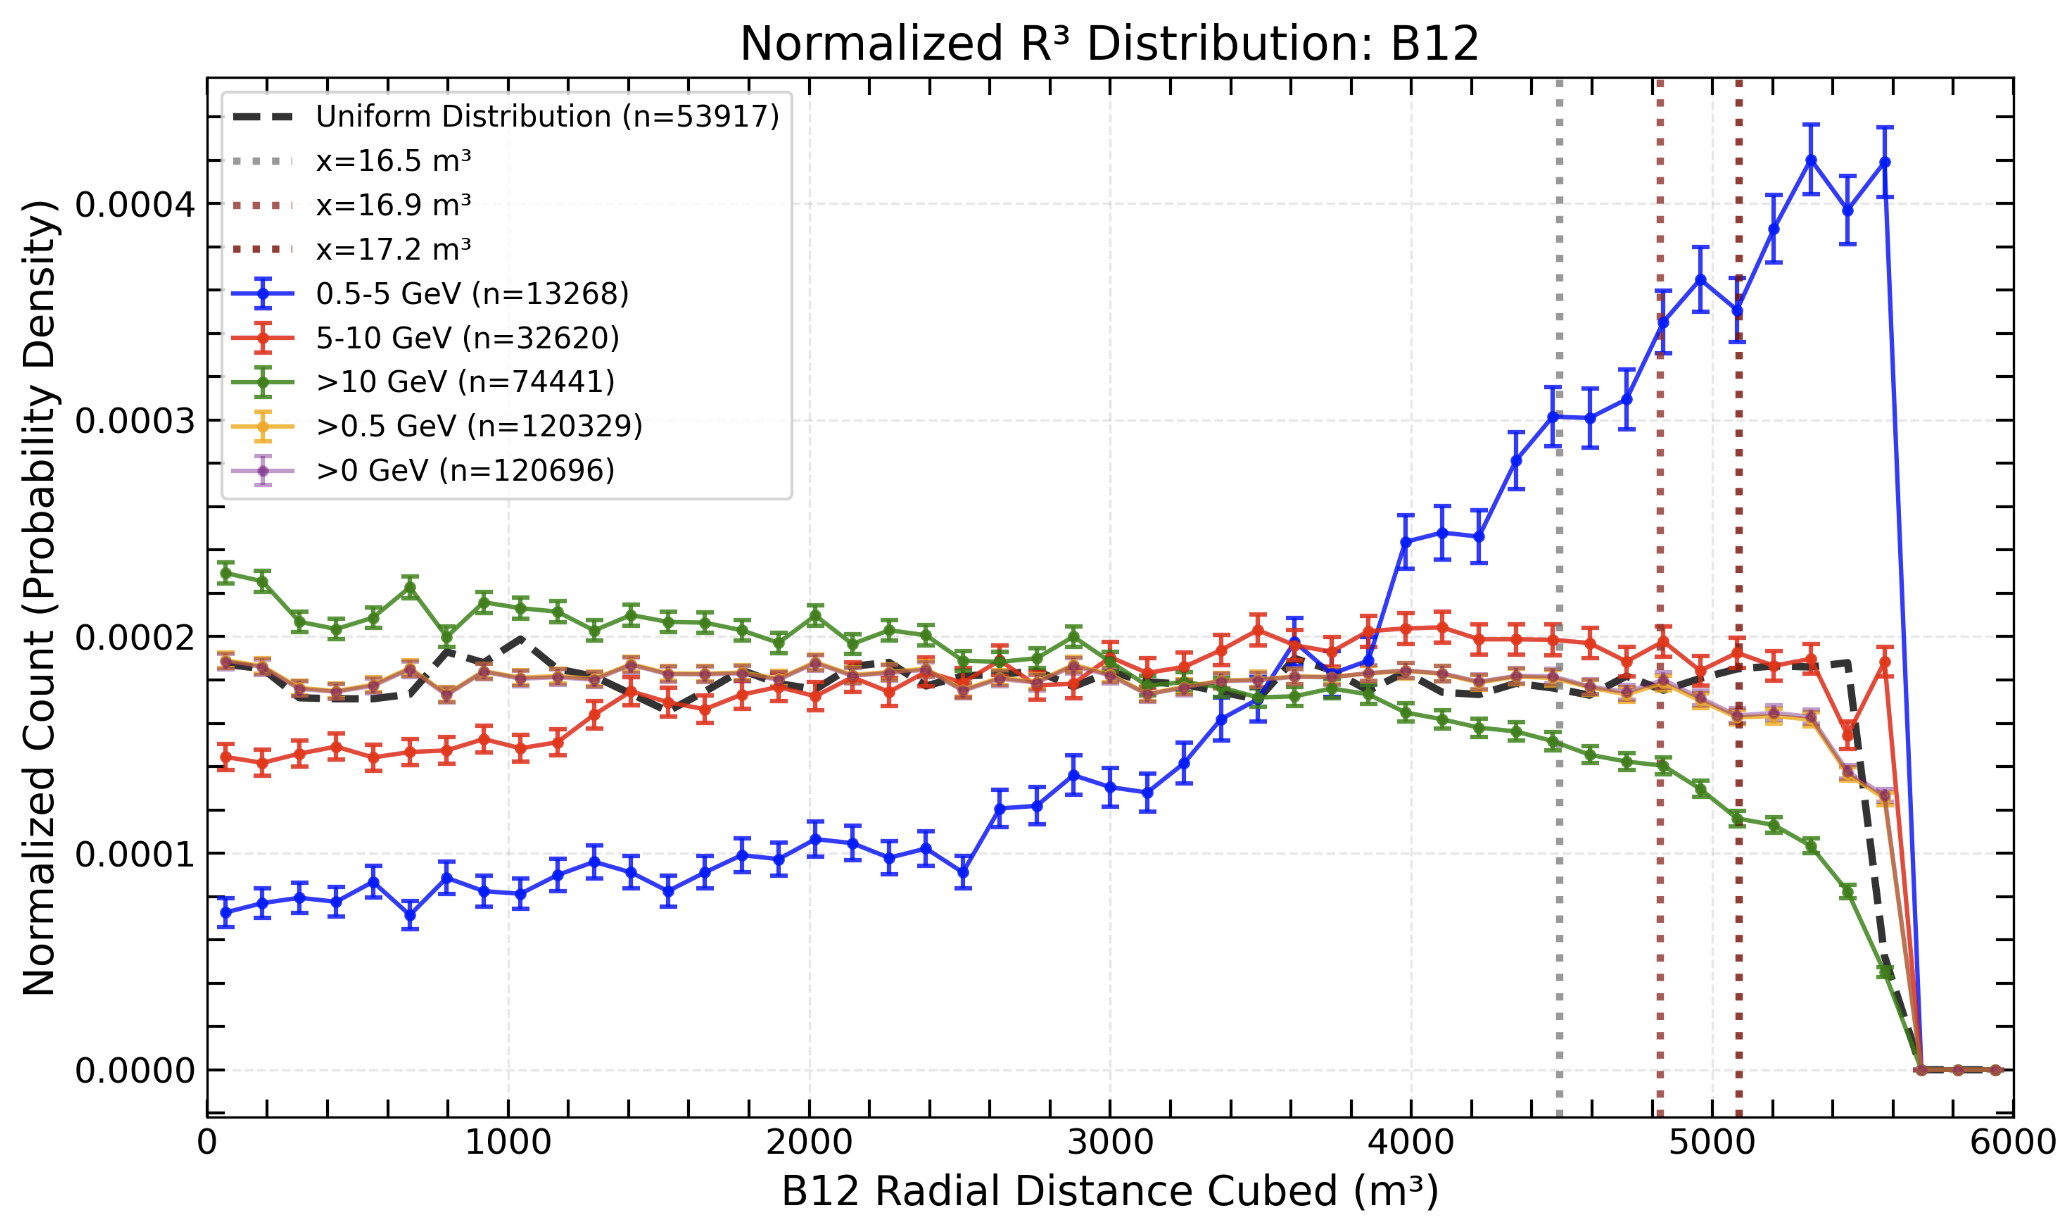
\includegraphics[width=\linewidth]{4_efficiency/B12_r3_mc.png}
    \caption{}
    \label{fig:B12_r3_mc}
  \end{subfigure}
  \hfill
  \begin{subfigure}[t]{0.43\textwidth}
    \centering
    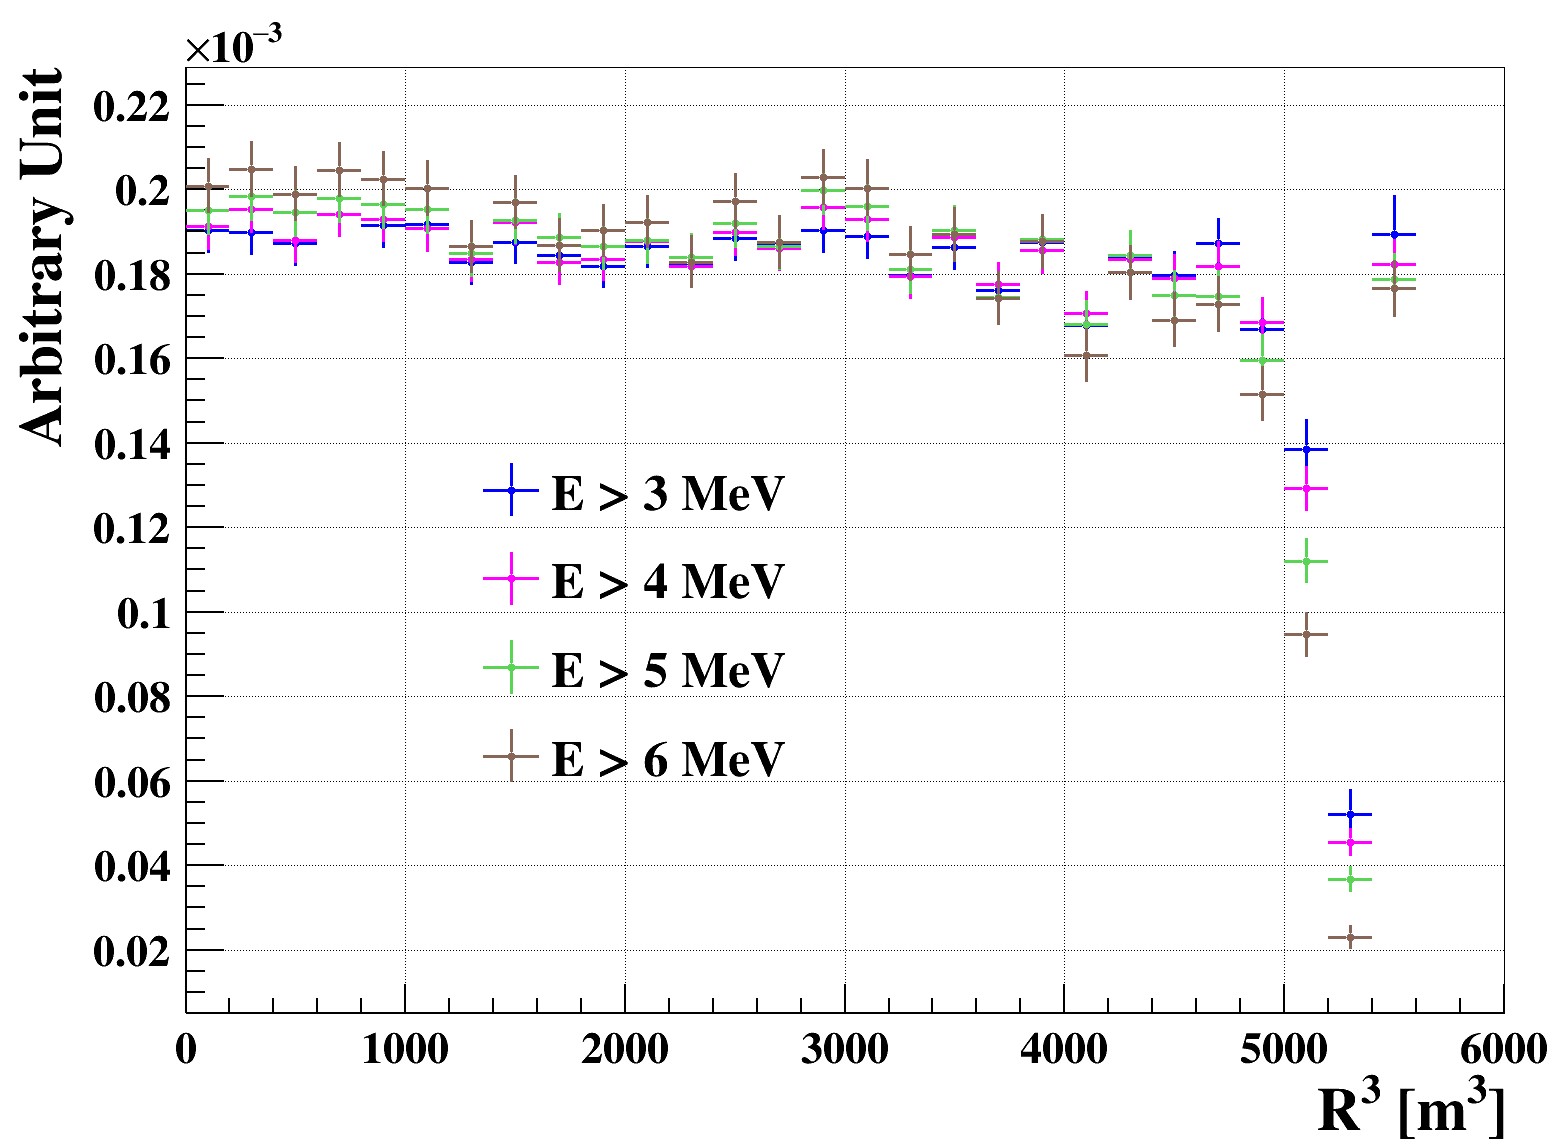
\includegraphics[width=\linewidth]{4_efficiency/B12_r3_data.png}
    \caption{}
    \label{fig:B12_r3_data}
  \end{subfigure}
  \caption{Radial vertex distribution of B12 in (a) MC and (b) data tagged by muons with reconstructed energy > 0.5 GeV.}
\end{figure}

As shown in Fig. \ref{fig:li9_r3_mc}, Li9 events produced by muons with deposited energy > 0.5 GeV have nearly uniform radial vertex distribution as well, which can be selected with neutron tagging in data.

\begin{figure}
    \centering
    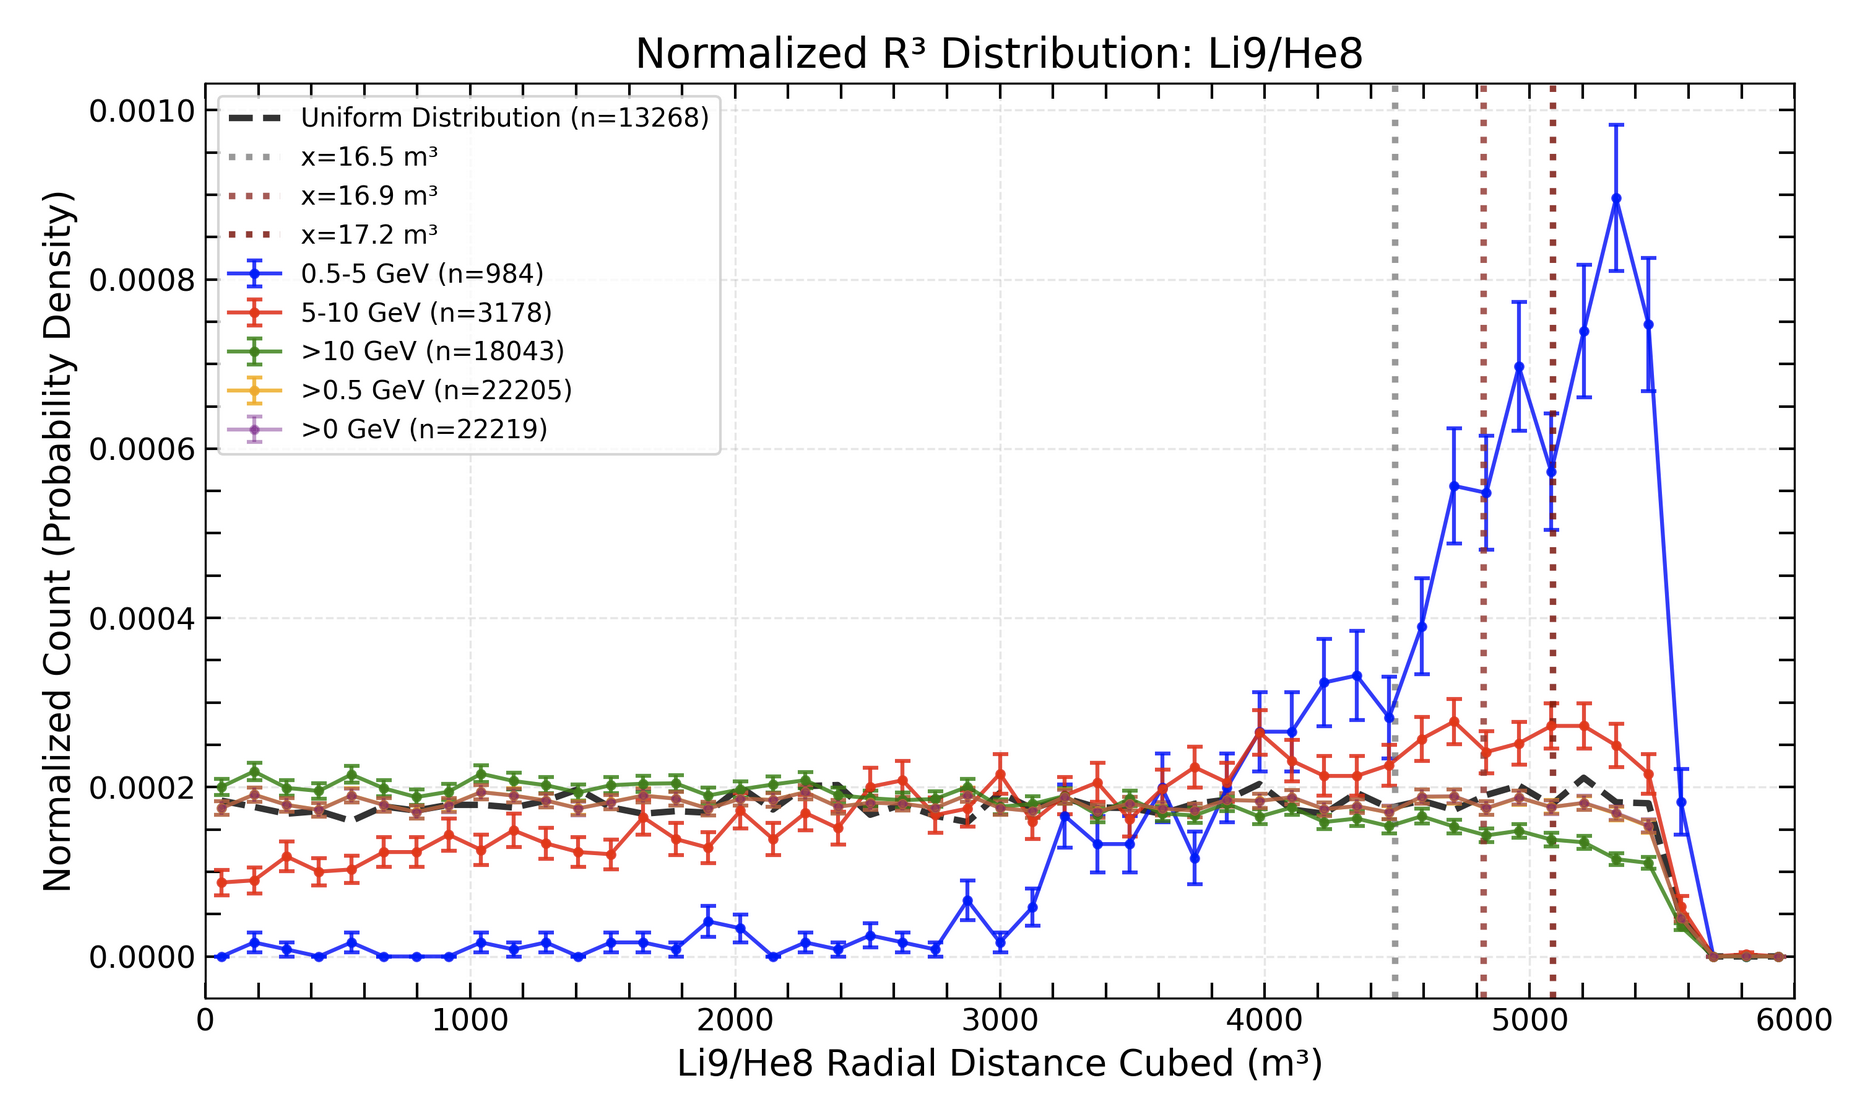
\includegraphics[width=0.5\linewidth]{4_efficiency/li9_r3_mc_v2.png}
    \caption{Radial vertex distribution of Li9 in MC.}
    \label{fig:li9_r3_mc}
\end{figure}

The efficiency also can be estimated with high-energy IBD samples, which is a more reasonable way [DocDB-15101].
To study the efficiency, FV cut is removed and high-energy cut is applied.
As shown in Fig. \ref{fig:IBD_candidate_spectra_fvCut}, after the cut ($E_p$ > 3.5 MeV), the accidental background should be negligible.
Additionally, SPN veto is removed to include more statistics and ensure uniform vertex distribution.
Fig. \ref{fig:IBD_r3_ed_beforeSPN} shows the $r^3$-vertex distribution after all above cuts, indicating nearly uniform radial distribution.


\begin{figure}[h]
  \centering
  \begin{subfigure}[t]{0.45\textwidth}
    \centering
    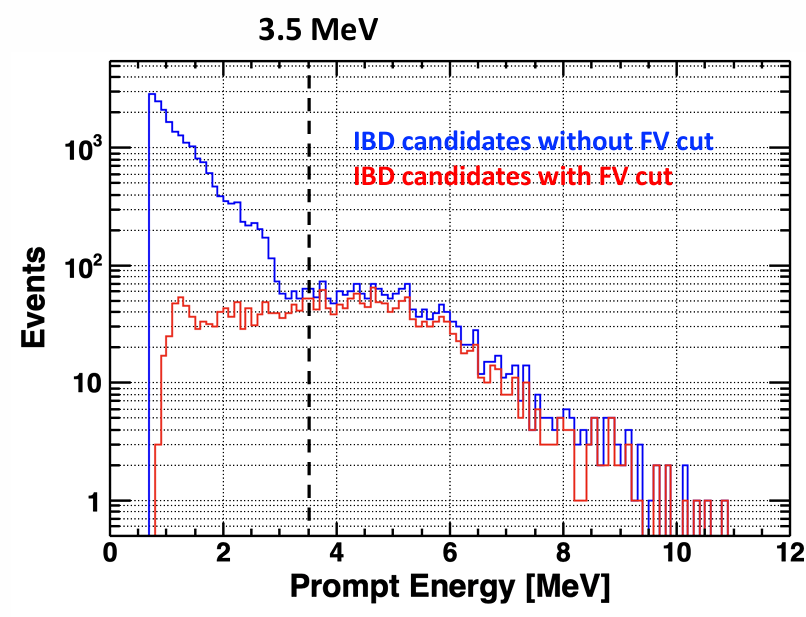
\includegraphics[width=\linewidth]{4_efficiency/IBD_candidate_spectra_fvCut.png}
    \caption{}
    \label{fig:IBD_candidate_spectra_fvCut}
  \end{subfigure}
  \hfill
  \begin{subfigure}[t]{0.5\textwidth}
    \centering
    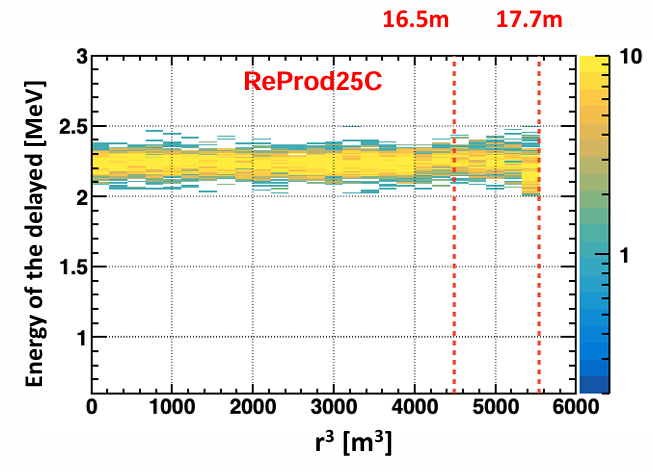
\includegraphics[width=\linewidth]{4_efficiency/IBD_r3_ed_beforeSPN.png}
    \caption{}
    \label{fig:IBD_r3_ed_beforeSPN}
  \end{subfigure}
  \caption{(a) Prompt spectra of IBD candidates without (blue line) and with (red line) FV cut. (b) $r^3$-$E_d$ distribution  of IBD candidate with prompt energy > 3.5 MeV and without FV cut and SPN veto.}
\end{figure}

Subsequently, the FV cut efficiency could be estimated as
\begin{equation}
    \epsilon^{\rm IBD}_{\rm FV} = \frac{\text{(IBDs with FV cut)}}{\text{(IBDs without FV cut)} \times (1+\epsilon_{\text{spill-out}})} (E_p > 3.5 \text{MeV})
    \label{eq:fv_eff_ibd}
\end{equation}
where $\epsilon_{\text{spill-out}}$ is the correction factor by spill-out effect where IBD neutrons could leak out LS region near the CD edge. Using 10 keV neutron MC samples provided by Peidong Yu, $\epsilon_{\text{spill-out}}$ is estimated as 2.4\%.
Then, the efficiency is calculated as ($79.61 \pm 0.58 (\text{stat.})$)\%.
The relative difference between geometric calculation and the estimation based on high-energy IBD sample is 1.2\%, which is consistent with each other.

The uncertainty could be estimated by the variation of the number density of IBD candidates near the FV edge.
As shown in Fig. \ref{fig:IBD_r3_density_omilrec}, the average density in FV is calculated as $d_{\text{inFV}}$ = 0.186 events/m$^3$, and the density in $r=[16, 16.5]$ m regions is $d_{r=[16, 16.5] m}$ =  0.15 events/m$^3$.
Then the uncertainty is estimated as 
\begin{equation}
    \sigma_{\rm FV} = 1 - \frac{V(r<16m) \times d_{\text{inFV}} + V(16<r<16.5m) \times d_{r=[16, 16.5] m}}{V(r<16.5m) \times d_{\text{inFV}}} = 1.6\%
    \label{eq:fv_eff_ibd}
\end{equation}

\begin{figure}
    \centering
    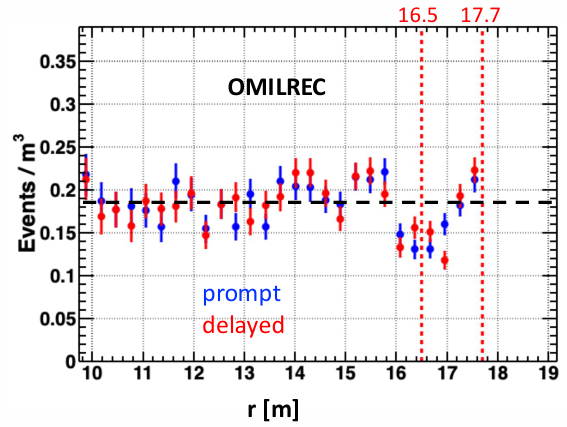
\includegraphics[width=0.5\linewidth]{4_efficiency/IBD_r3_density_omilrec.png}
    \caption{The number density of IBD candidates along radial direction. The black dashed line represents the average density in FV.}
    \label{fig:IBD_r3_density_omilrec}
\end{figure}


\subsubsection{Muon veto}
To suppress cosmogenic backgrounds, three types of muon veto strategies are designed:
\begin{itemize}
    \item WP and CD muon veto: apply on delayed signals over the whole target volume.
    \item Spallation neutron (SPN) veto: apply on delayed signals inside the sphere around spallation neutron events.
    \item Muon track veto (not included in this note): apply on delayed signals around muon tracks.
\end{itemize}

For the first type of muon veto, the corresponding efficiency is calculated as the ratio of live time to DAQ time:
\begin{equation}
    \epsilon_{\mu,\text{wholeV}} = \frac{(\text{Live time after first type of veto})}{(\text{DAQ time})} = 95.55\%
    \label{eq:muon_veto_eff_all_volume}
\end{equation}
The uncertainty mainly comes from the time precision ($\sim$ 8 ns), which is negligible.

Since the SPN veto is just applied on specific volume, the above estimation method is not applicable any more.
A novel grid method, named as XYZFrame, is proposed to calculate SPN veto efficiency with negligible uncertainty [DocDB-14949].
In this method, the whole target volume is divided into cubic cells whose radius can be optimized according to the resolution of vertex reconstruction, as shown in Fig. \ref{fig:xyzframe_sketch}. 
Then, we calculate their live time by regarding each cell as a sub-detector and integrate over all the cell to get the total live time and efficiency.
%Fig. \ref{fig:muon_spn_veto_eff} shows the calculated results.

\begin{figure}
    \centering
    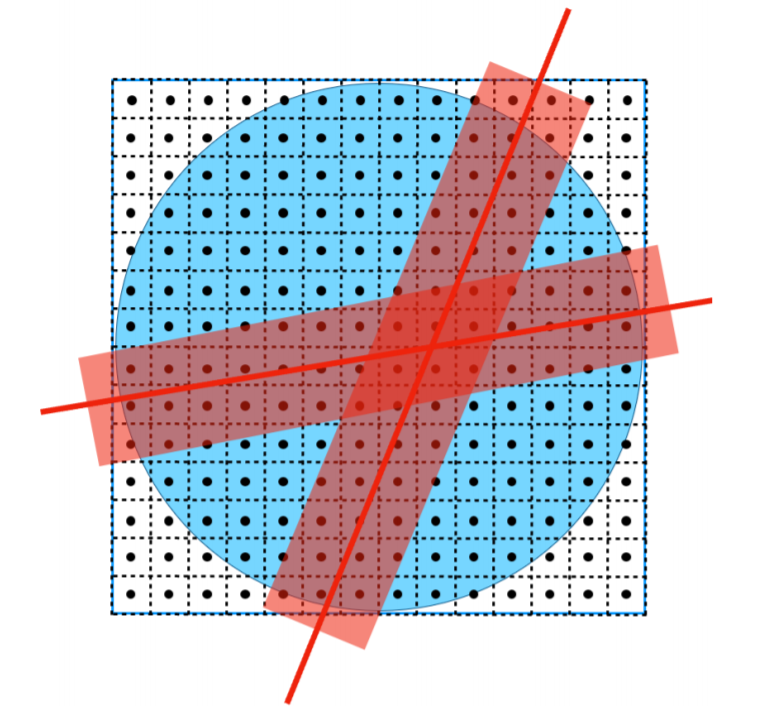
\includegraphics[width=0.5\linewidth]{4_efficiency/xyzframe_sketch.png}
    \caption{Sketch of XYZFrame method for the calculation of the SPN veto efficiency.}
    \label{fig:xyzframe_sketch}
\end{figure}

% \begin{figure}
%     \centering
%     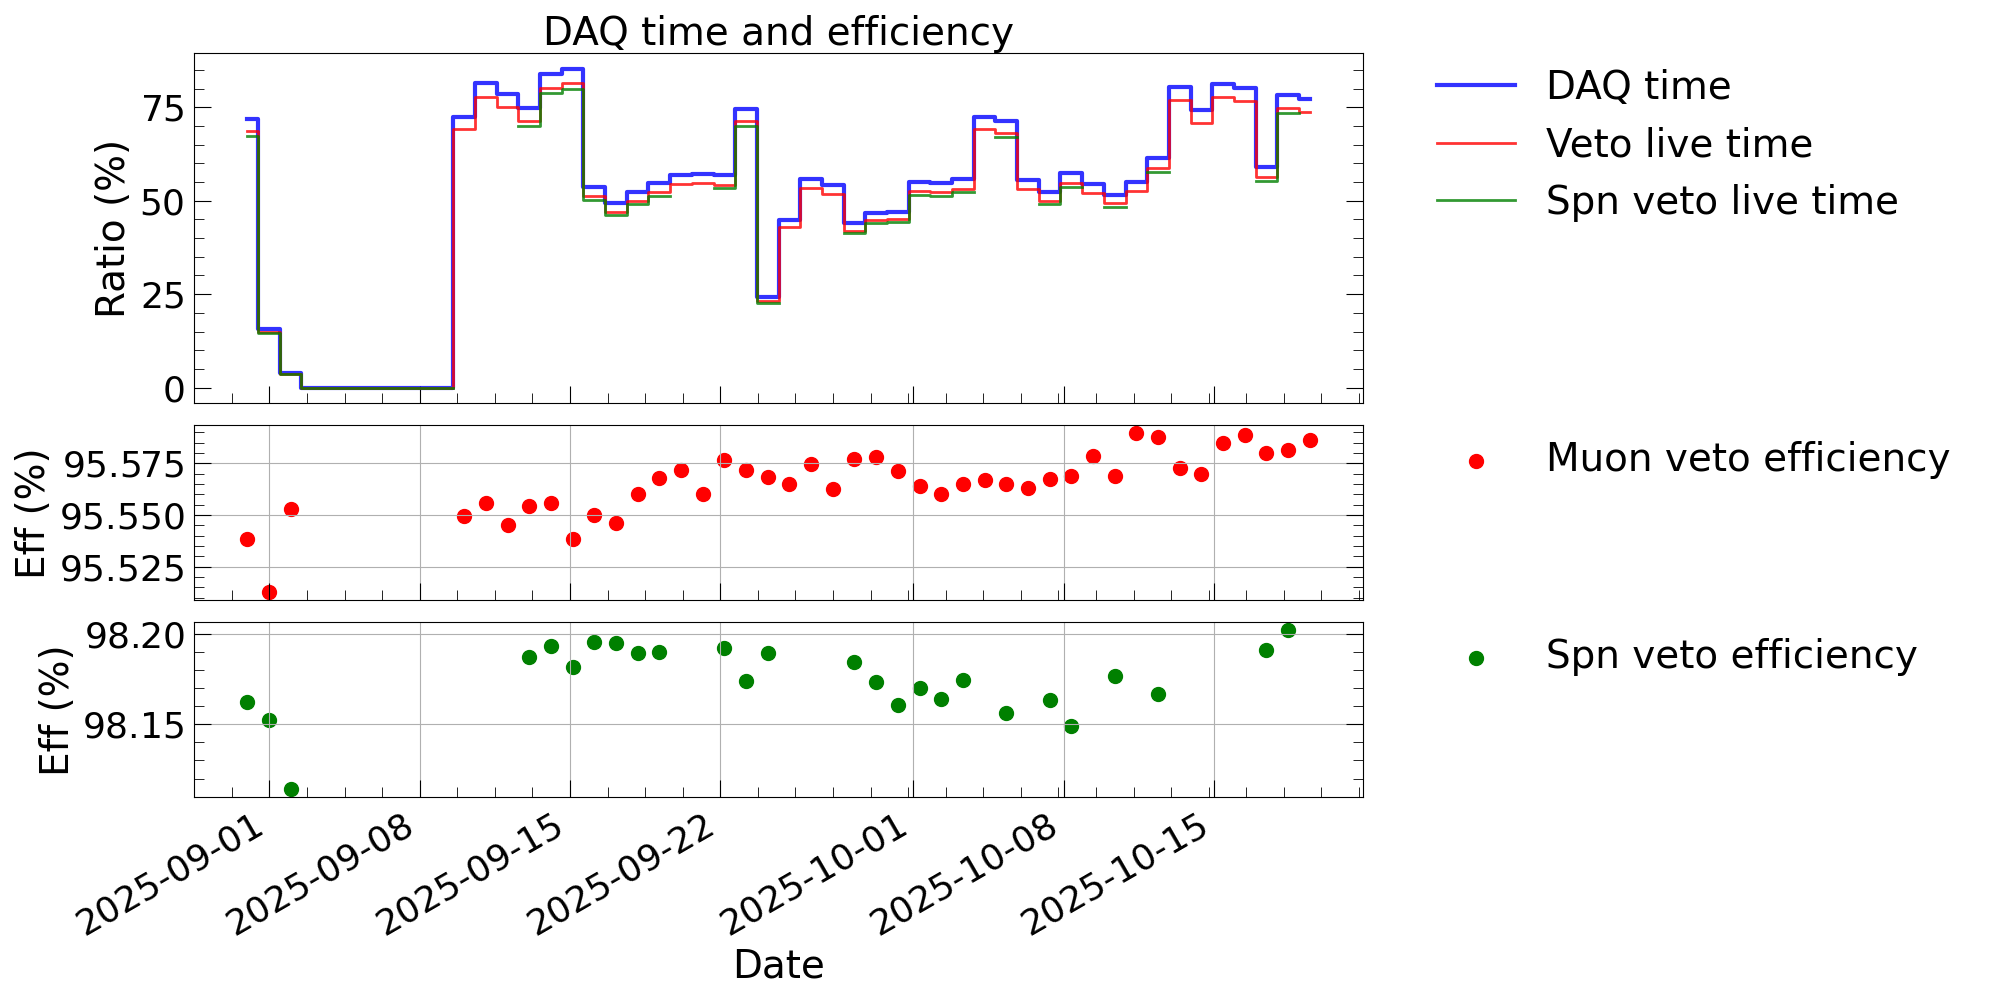
\includegraphics[width=0.95\linewidth]{4_efficiency/muon_spn_veto_eff.png}
%     \caption{Time variation of calculated muon veto and SPN veto efficiency (updating).}
%     \label{fig:muon_spn_veto_eff}
% \end{figure}


\subsubsection{Multiplicity cut}
In principle, the multiplicity cut efficiency can be calculated with the single rate analytically:
\begin{equation}
    \epsilon_{m} = e^{-(3R_{s}+3R_{c}+R_{\mu})T_{\rm corr}} \left( \int^{T_{\rm veto}}_{0} R_{\mu} e^{-R_{\mu}t_{1}} e^{-\int^{T^{\rm veto}}_{T_{\rm veto}-t_{1}} f(t_{2})dt_{2} } dt_{1} + e^{-R_{\mu}T_{\rm veto}} \right)
    \label{eq:multi_eff_cal}
\end{equation}

The efficiency also can be calculated with live time method with negligible uncertainty, as shown in Fig. \ref{fig:multi_eff_cal} [DocDB-14397].
Fig. \ref{fig:multi_eff_vs_time} shows the calculated results.

\begin{figure}
    \centering
    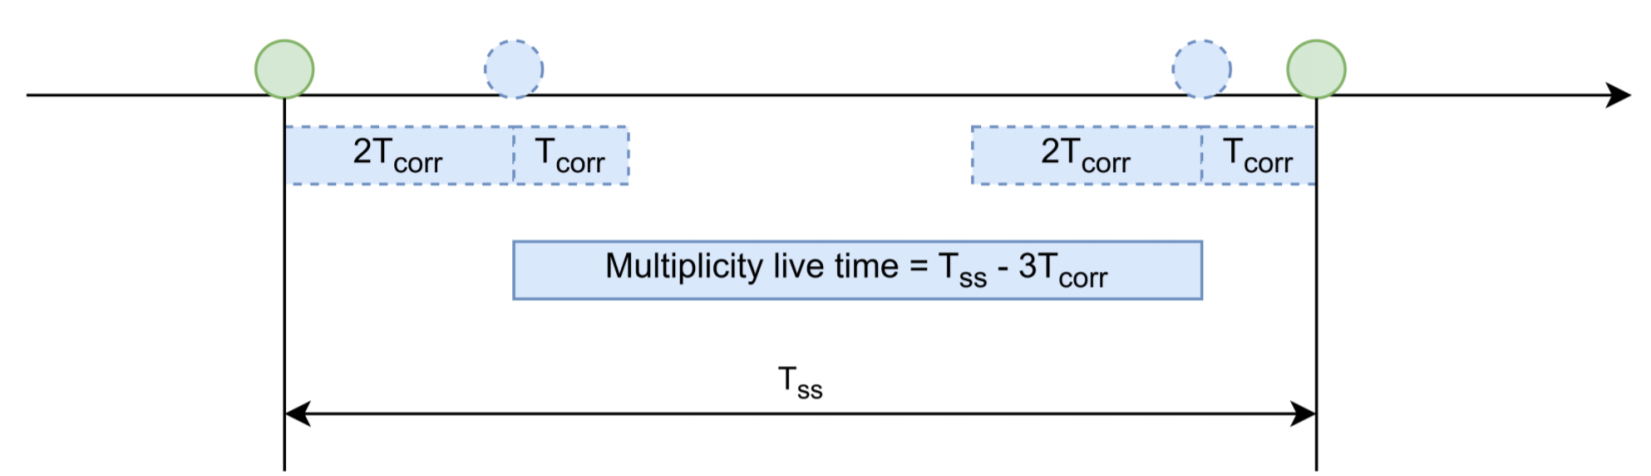
\includegraphics[width=0.95\linewidth]{4_efficiency/multi_eff_cal.png}
    \caption{Sketch for the calculation of the multiplicity cut efficiency. Green solid circles represent real events, and bule dashed circles imaginary signals.}
    \label{fig:multi_eff_cal}
\end{figure}

\begin{figure}
    \centering
    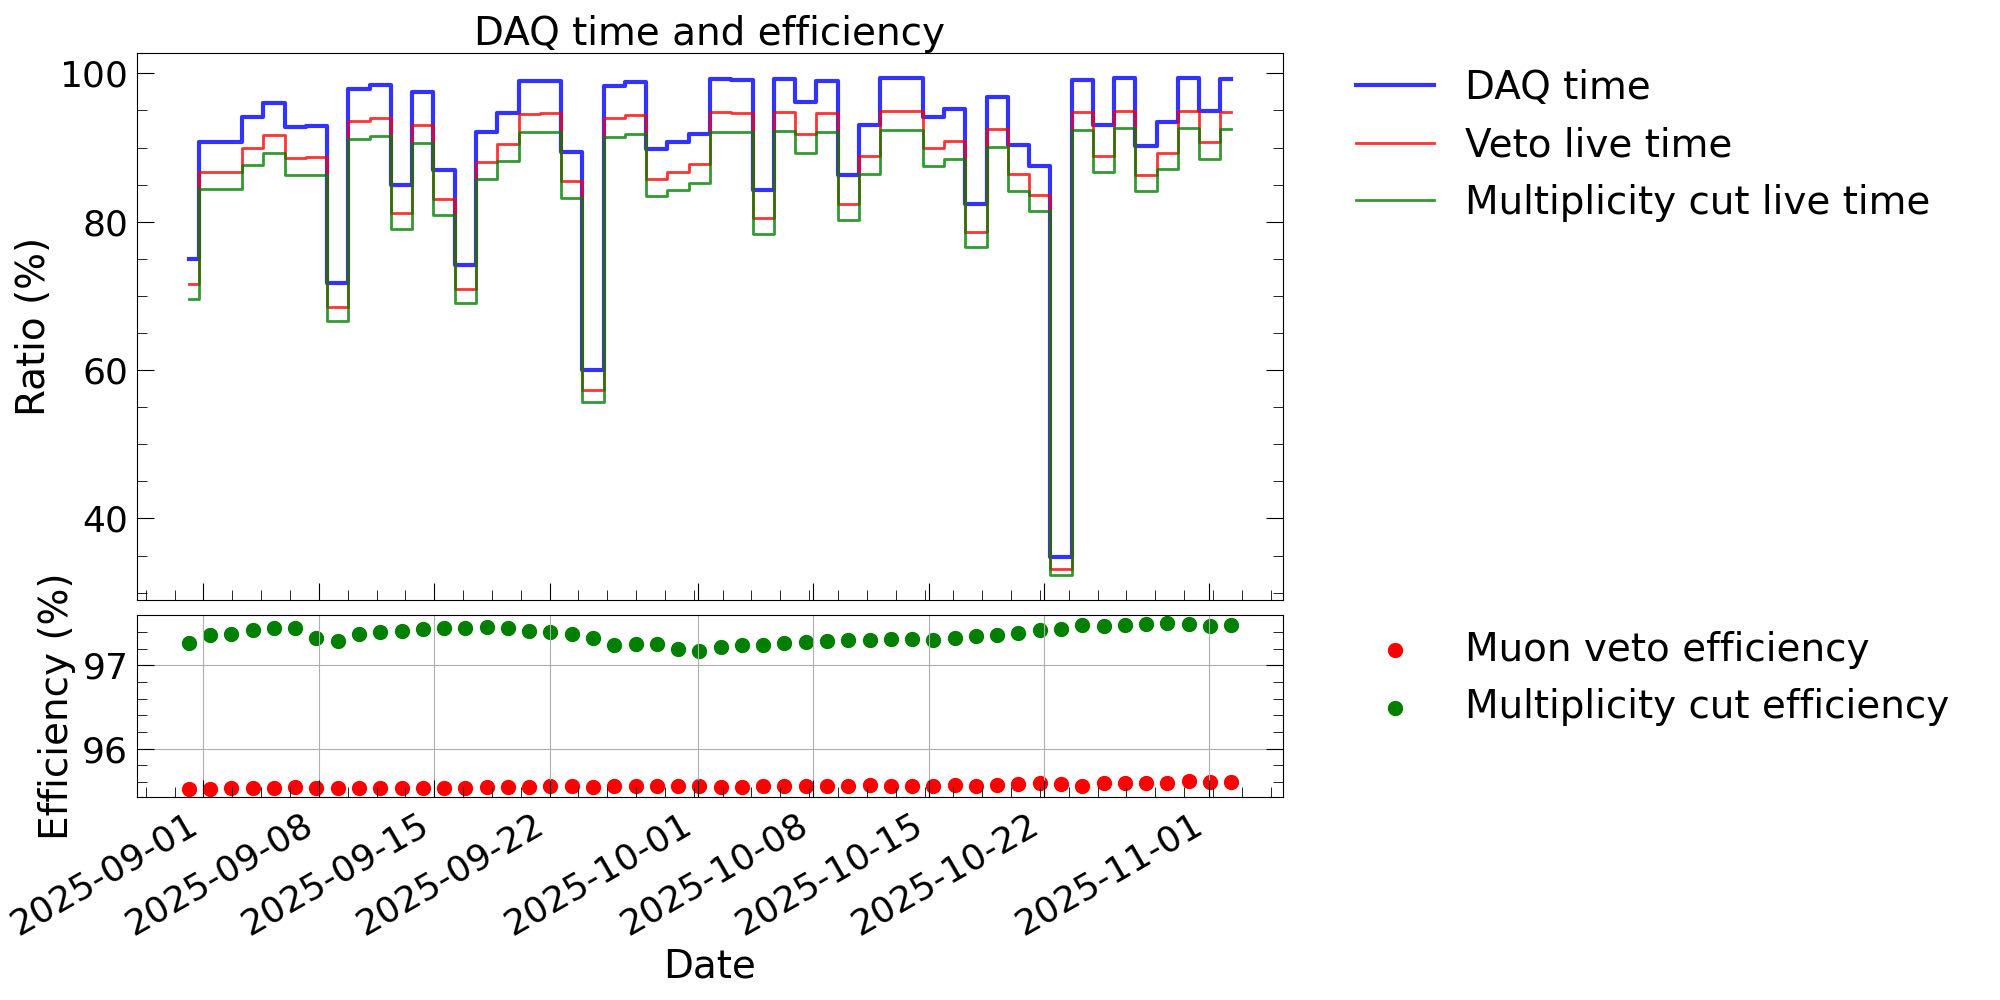
\includegraphics[width=0.95\linewidth]{4_efficiency/multi_eff_vs_time.jpg}
    \caption{Time variation of calculated multiplicity cut efficiency.}
    \label{fig:multi_eff_vs_time}
\end{figure}


\subsubsection{Prompt energy cut}
The prompt energy of IBDs is constrained within (0.7, 12) MeV. The in-efficiency mainly comes from two parts: energy leakage and energy resolution.

With the tight FV cut, the energy leakage effect is negligible, as confirmed with MC samples and shown in \ref{fig:ep_mc_all}, \ref{fig:ep_mc_169} and \ref{fig:ep_mc_165}.

\begin{figure}[h]
  \centering
  \begin{subfigure}[t]{0.32\textwidth}
    \centering
    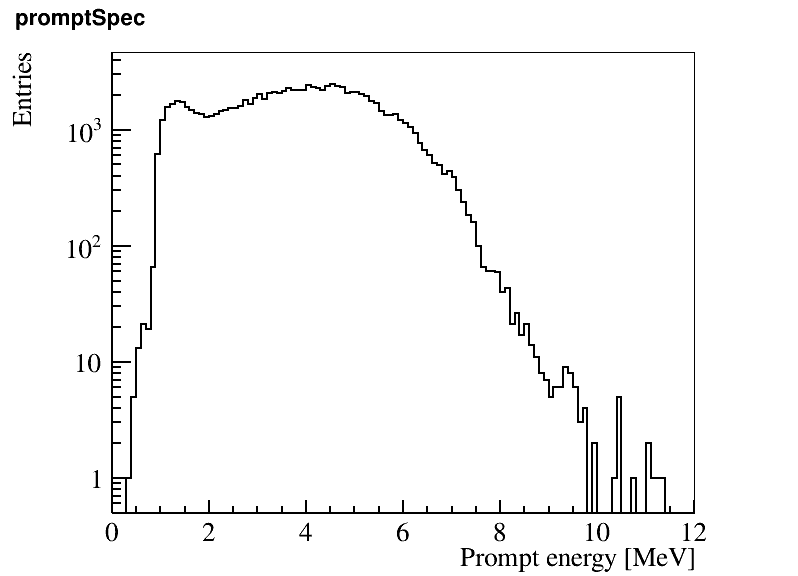
\includegraphics[width=\linewidth]{4_efficiency/promptSpec_logy_mc_ibd_all.png}
    \caption{}
    \label{fig:ep_mc_all}
  \end{subfigure}
  \hfill
  \begin{subfigure}[t]{0.32\textwidth}
    \centering
    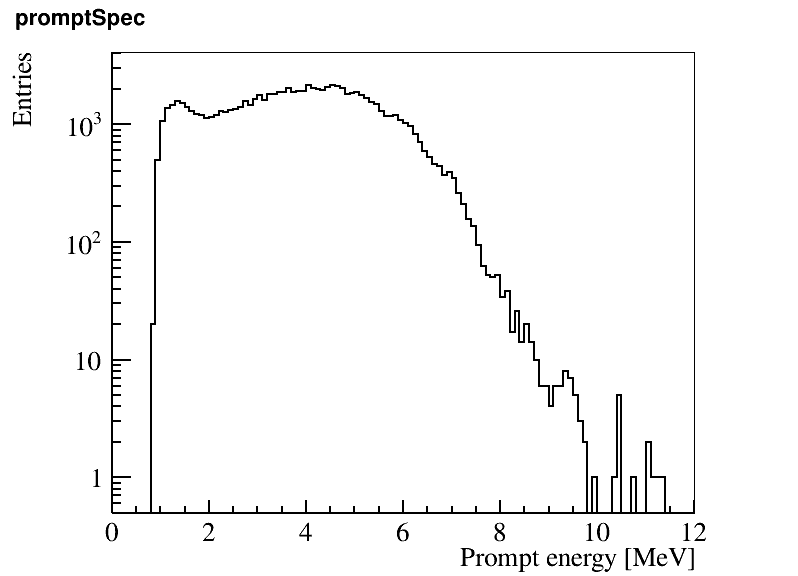
\includegraphics[width=\linewidth]{4_efficiency/promptSpec_logy_mc_ibd_169.png}
    \caption{}
    \label{fig:ep_mc_169}
  \end{subfigure}
  \hfill
  \begin{subfigure}[t]{0.32\textwidth}
    \centering
    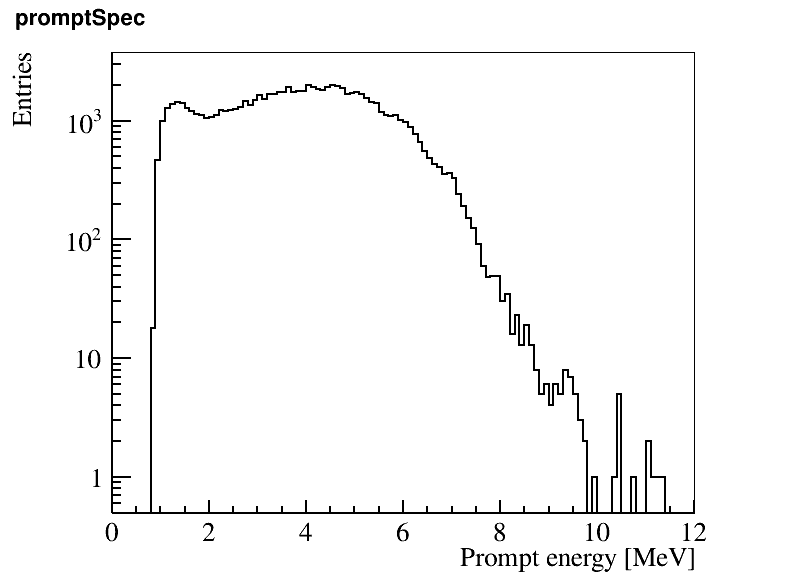
\includegraphics[width=\linewidth]{4_efficiency/promptSpec_logy_mc_ibd_165.png}
    \caption{}
    \label{fig:ep_mc_165}
  \end{subfigure}
  \caption{Prompt spectra of MC IBDs with different FV cuts: (a) no FV cut, (b) FV < 16.9 m and (c) FV < 16.5 m.}
\end{figure}

To study the in-efficiency caused by the energy resolution, we use calibration data of Ge68 source with two 0.511 MeV $\gamma$s emitted, which is corresponding to the lowest energy of IBDs without energy leakage.
As shown in the Fig. \ref{fig:Ge68_spec_x0y0z0_fit}, one single Gaussian function is used in the fitting to get the peak energy $\mu$ and resolution $\sigma$.
Then the lowest reconstructed prompt energy is estimated as $\sim$ 0.77 MeV for OEC energy and $\sim$ 0.75 MeV for OMILREC energy, which are both higher than the energy threshold of 0.7 MeV.

\begin{figure}
    \centering
    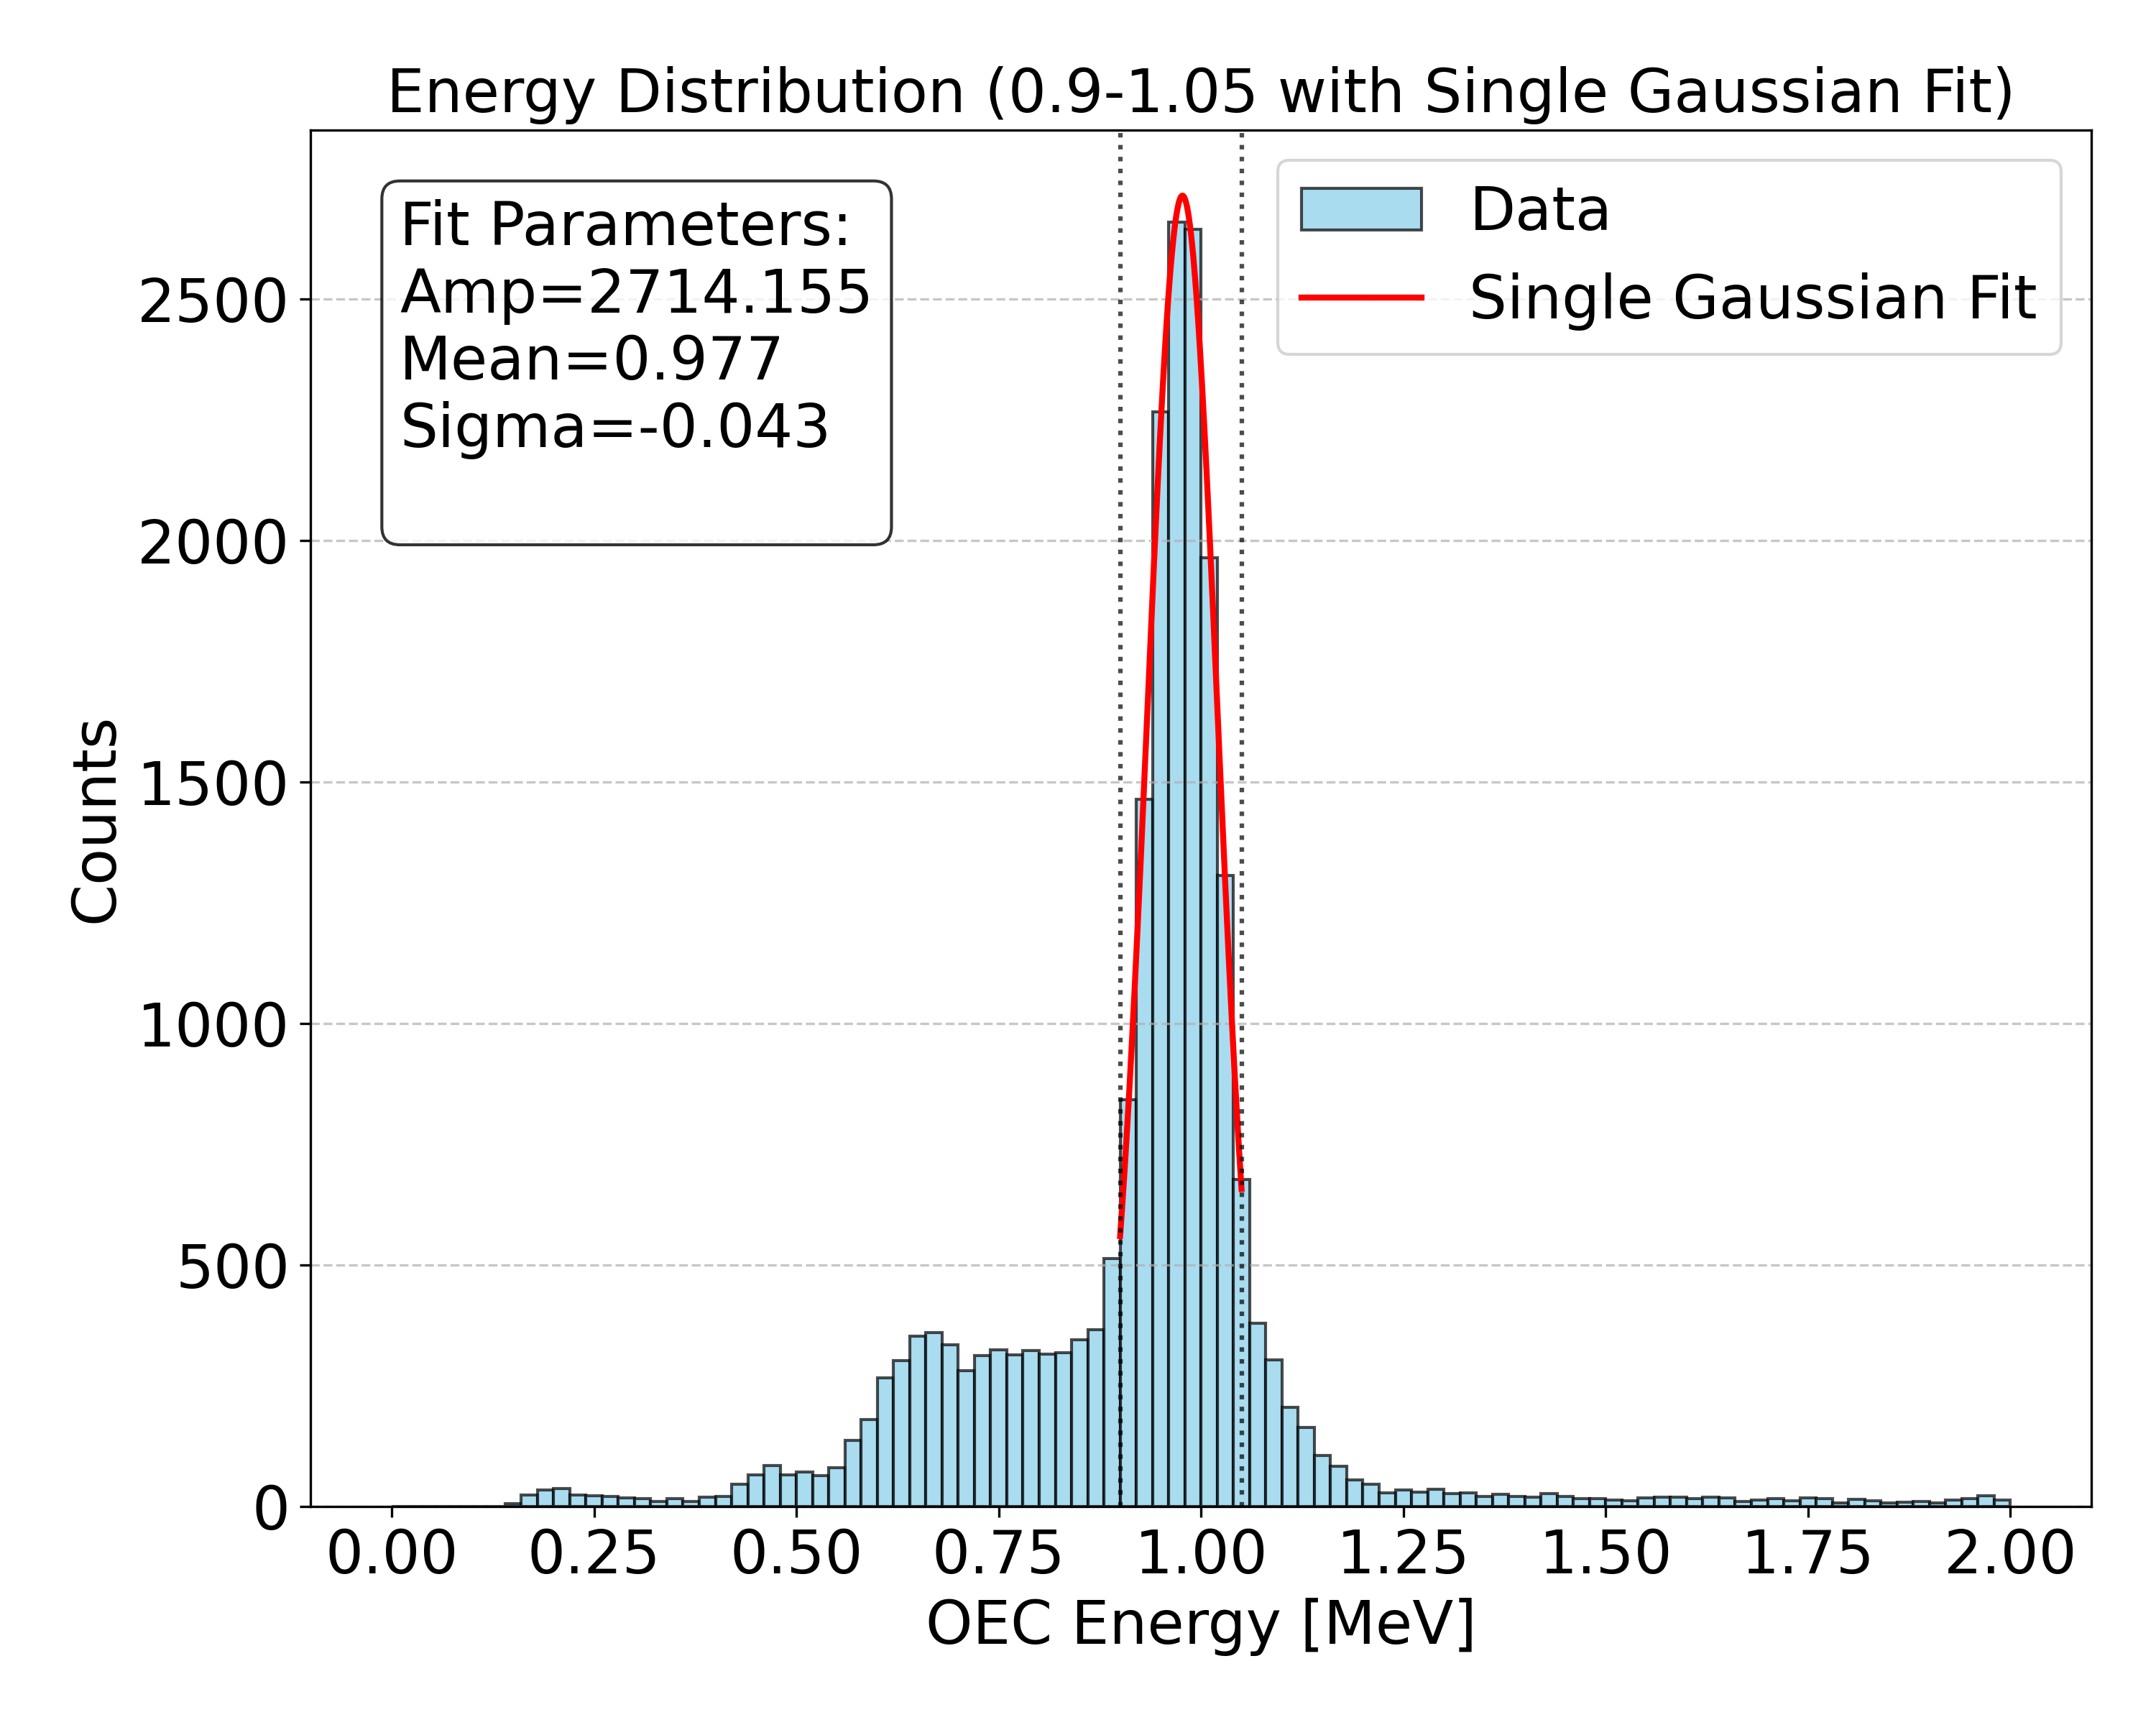
\includegraphics[width=0.5\linewidth]{4_efficiency/Ge68_spec_x0y0z0_fit.png}
    \caption{Energy spectrum of $^{68}$Ge source at CD center. The full-energy peak is fitted with single Gaussian function.}
    \label{fig:Ge68_spec_x0y0z0_fit}
\end{figure}

In summary, the in-efficiency and the corresponding uncertainty of prompt energy cut are both negligible in our selections.

\subsubsection{Delayed energy cut}
As discussed in the previous section and shown in Fig. \ref{fig:ed_mc_all}, \ref{fig:ed_mc_169} and \ref{fig:ed_mc_165}, the energy leakage effect is negligible with this tight FV cut.
Thus, we use a single Gaussian function to fit the delayed spectrum, as shown in Fig. \ref{fig:delayedSpec_ibd}.
Then the efficiency of delayed energy cut is calculated with the fitting function as 
\begin{equation}
    \epsilon_{ed} = \frac{N(2.0~{\rm MeV} < E_{d} < 2.5~{\rm MeV})}{N(\text{Without Ed cut})} = 99.99\%
    \label{eq:ed_eff}
\end{equation}

\begin{figure}[h]
  \centering
  \begin{subfigure}[t]{0.32\textwidth}
    \centering
    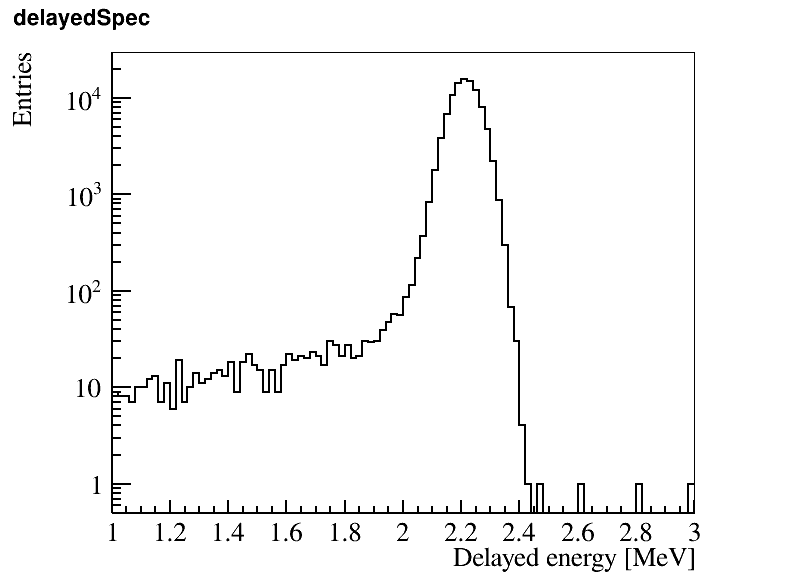
\includegraphics[width=\linewidth]{4_efficiency/delayedSpec_logy_mc_ibd_all.png}
    \caption{}
    \label{fig:ed_mc_all}
  \end{subfigure}
  \hfill
  \begin{subfigure}[t]{0.32\textwidth}
    \centering
    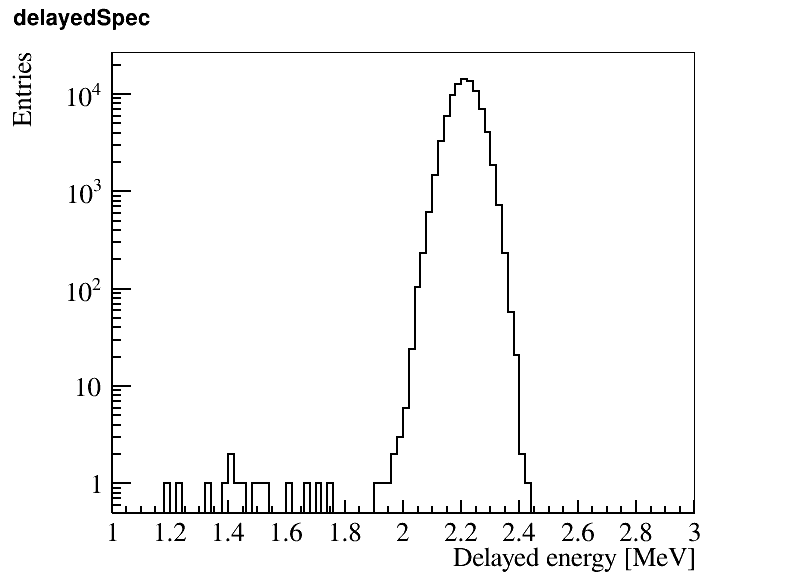
\includegraphics[width=\linewidth]{4_efficiency/delayedSpec_logy_mc_ibd_169.png}
    \caption{}
    \label{fig:ed_mc_169}
  \end{subfigure}
  \hfill
  \begin{subfigure}[t]{0.32\textwidth}
    \centering
    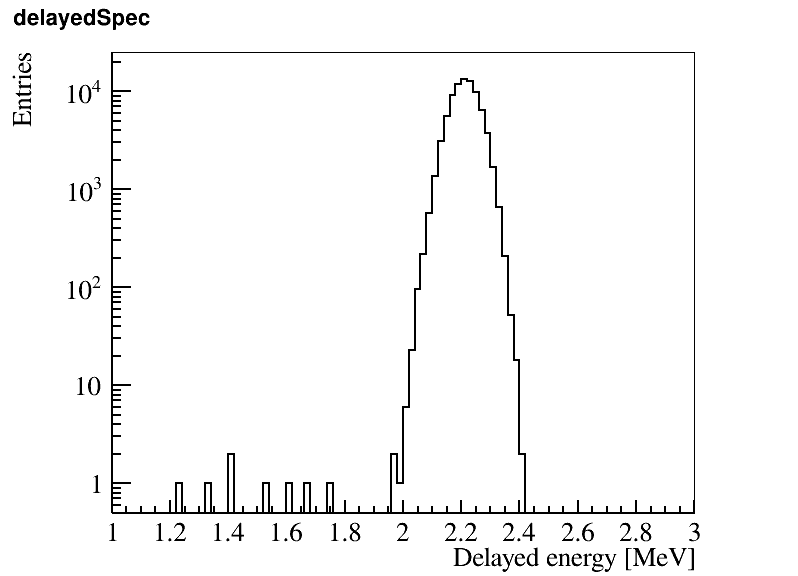
\includegraphics[width=\linewidth]{4_efficiency/delayedSpec_logy_mc_ibd_165.png}
    \caption{}
    \label{fig:ed_mc_165}
  \end{subfigure}
  \caption{Delayed spectra of MC IBDs with different FV cuts: (a) no FV cut, (b) FV < 16.9 m and (c) FV < 16.5 m. Significant energy leakage is found without any FV cut and negligible effect exists with FV < 16.9 m or FV < 16.5 m.}
\end{figure}

The analysis of the corresponding systematic uncertainty is still under way. 
It mainly comes from the fitting strategy and energy response related uncertainty which will lead to the distortion of spectrum shape.
Since the efficiency is high enough, the systematic uncertainty is set to 0.1\% directly.

\begin{figure}
    \centering
    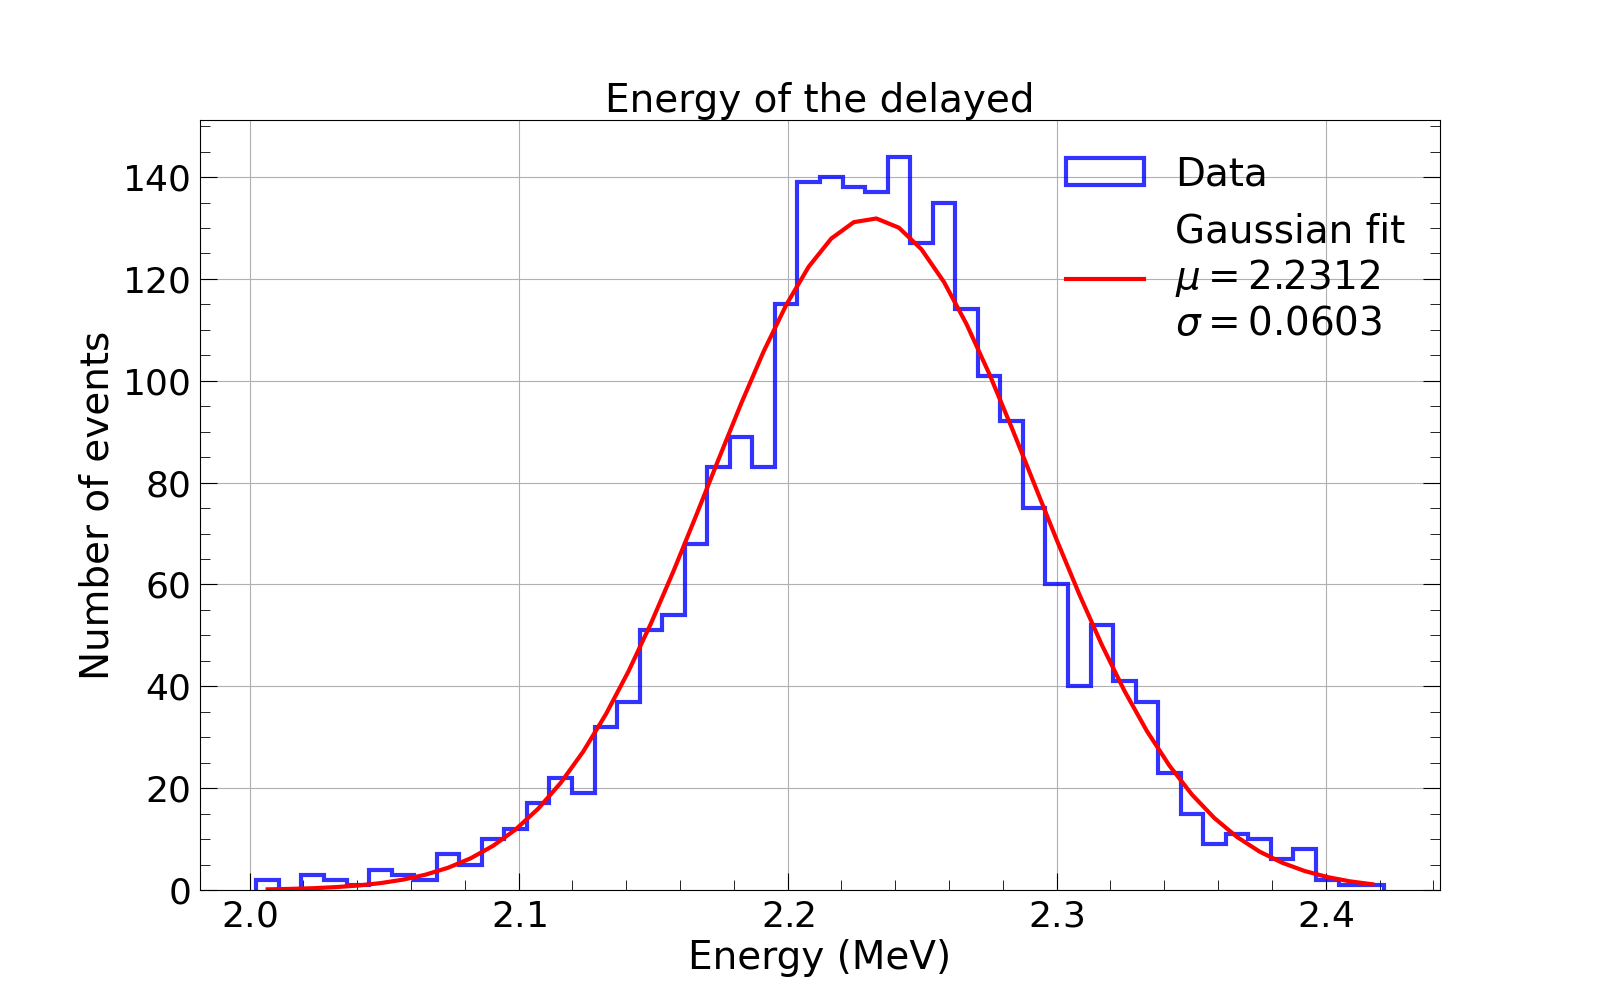
\includegraphics[width=0.5\linewidth]{2_selection/h_ibd_e_d.png}
    \caption{Delayed spectrum of IBD candidates. The data is fitted with single Gaussian function.}
    \label{fig:delayedSpec_ibd}
\end{figure}

Noting that the efficiency estimation is based on the OEC energy, the efficiency for OMILREC reconstruction will be re-calculated once enough re-production data and fine-tuning MC samples are ready.


\subsubsection{Time interval cut}
The time interval between prompt and delayed signals are composed of two parts, neutron thermalization ($\sim$ 4 $\mu$s) and neutron capture on hydrogen (nH) ($\sim$ 220 $\mu$s).
As a preliminary study, we neglect the contribution from the thermalization which is much faster compared to neutron capture and has small effect on the estimation of the efficiency.
In this case, the time constant should be identical for AmC and IBD.
By fitting the time interval distribution, the time constant $\tau$ can be obtained from these two samples, as shown in Fig. \ref{fig:dt_ibd} and Fig. \ref{fig:dt_AmC}. Then, the efficiency of dt cut can be calculated with the fitting function as
\begin{equation}
    \epsilon_{dt} = \frac{N(5~\mu s<dt<1000~\mu s)}{N(\text{Without dt cut})} = 96.80\%
    \label{eq:dt_eff}
\end{equation}

\begin{figure}[h]
  \centering
  \begin{subfigure}[t]{0.45\textwidth}
    \centering
    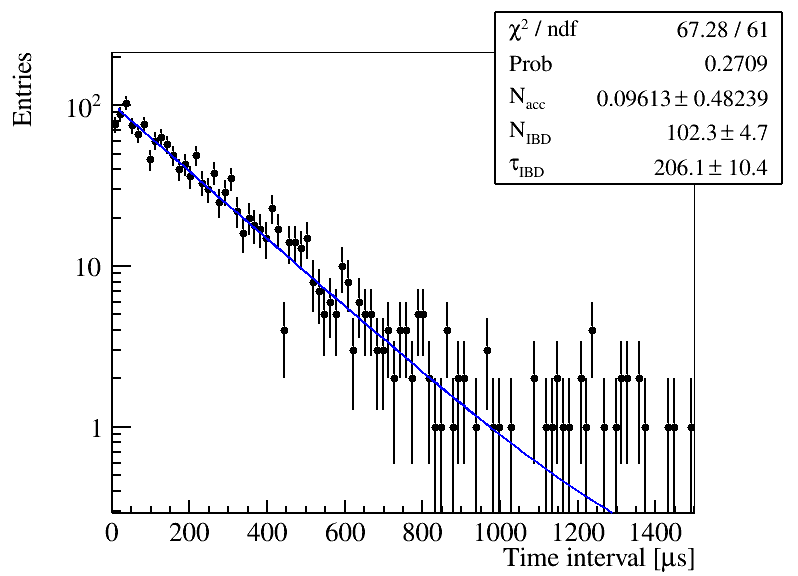
\includegraphics[width=\linewidth]{4_efficiency/dt_ibd.png}
    \caption{}
    \label{fig:dt_ibd}
  \end{subfigure}
  \hfill
  \begin{subfigure}[t]{0.45\textwidth}
    \centering
    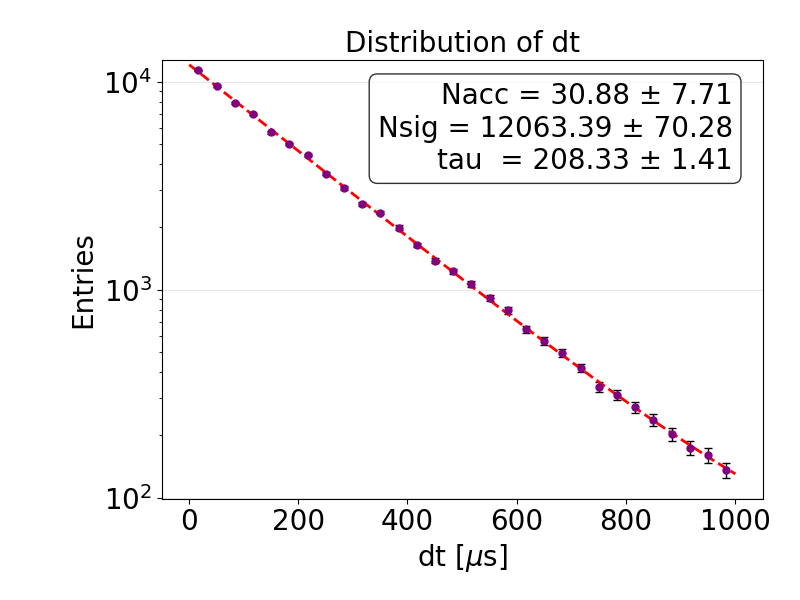
\includegraphics[width=\linewidth]{4_efficiency/dt_AmC_fit.png}
    \caption{}
    \label{fig:dt_AmC}
  \end{subfigure}
  \caption{Time interval distribution of (a) IBDs and (b) AmC correlated events. The data is fitted with an exponential decay function plus an constant.}
\end{figure}

The systematic uncertainty mainly comes from the time precision ($\sim$ 8 ns) and the fitting error of the time constant.
The time precision has negligible effect on the efficiency.
For the second factor, we compared the fitting time constant $\tau$ with AmC and IBD samples, and found the relative difference as $\sim$ 1\%. Then, it leads to the relative difference of the efficiency as $\sim$ 0.02\%, which is taken as the systematic uncertainty.


\subsubsection{Relative distance cut}
In this section, we use IBD candidate sample to estimate the efficiency of relative distance (dr) cut. 

To make an unbiased estimation, backgrounds should be removed from the sample.
After the standard IBD selection, the main backgrounds include Li9, geo-neutrinos, world reactor neutrinos, accidental background and so on. Geo-neutrinos and world reactor neutrinos have the same dr distribution as IBDs', which has not effect on the estimation.
As shown in Fig. \ref{fig:dr_ibd_li9_amc_mc}, IBD and Li9 have the same distribution of relative distance within the uncertainty. Thus, it's acceptable to reserve Li9 in the sample as well. 
However, the dr distribution of accidental background is flat, which will bias the estimation.
To remove this background, more strict selections are applied: $E_p$ > 1.5 MeV, and $dt$ < 600 $\mu$s.
For comparison, distributions of MC IBD [DocDB-13483] and AmC are shown in Fig. \ref{fig:dr_ibd_li9_amc_mc} as well. 

\begin{figure}
    \centering
    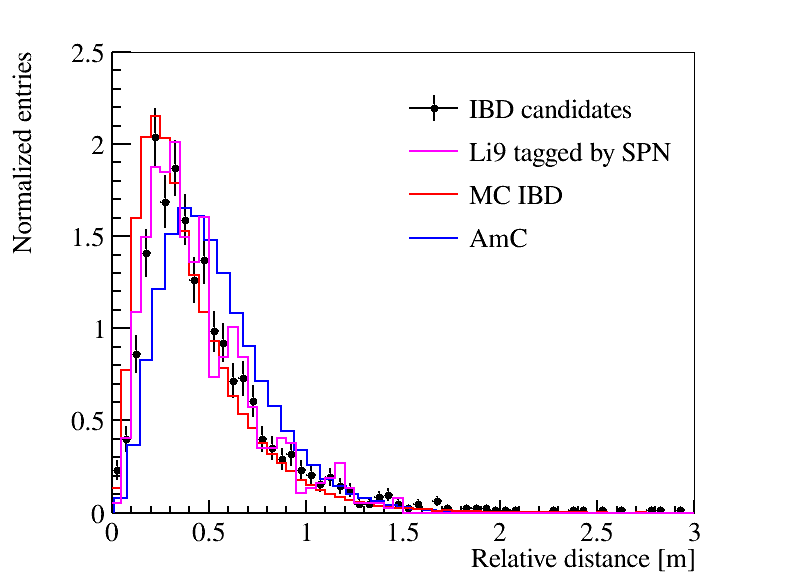
\includegraphics[width=0.5\linewidth]{4_efficiency/dr_ibd_li9_amc_mc.png}
    \caption{Relative distance distribution of IBD candidates with strict selections (black points), Li9 tagged by SPN (magenta line), MC IBDs (red line) and AmC correlated events (blue line).}
    \label{fig:dr_ibd_li9_amc_mc}
\end{figure}

With the above sample, the efficiency could be estimated as
\begin{equation}
    \epsilon_{dr} = \frac{N(dr<1.5~{\rm m})}{N(dr<3~{\rm m})} = 98.28\%
    \label{eq:dr_eff}
\end{equation}
According to MC studies, all IBDs have the relative distance dr < 3 m. Meanwhile, larger upper limit of the denominator in Eq. \ref{eq:dr_eff} will include more backgrounds and then leads to biased results.

The systematic uncertainty is estimated as the relative difference between IBD candidate and MC samples, which leads to 0.1\% uncertainty.


\subsubsection{Hydrogen-carbon capture ratio}
Inside LS region, IBD neutrons will be captured by hydrogens (nH) or carbons (nC), while in this technote only nH events are used.
To figure out the hydrogen-carbon capture ratio $\epsilon_{\text{nHCap}}$, we select AmC events with larger delayed energy region extending to 6 MeV, as shown in Fig. \ref{fig:full_delayed_spec_AmC}.
Then the ratio is estimated as
\begin{equation}
    \epsilon_{\text{nHCap}} = \frac{N(E_d<\text{3 MeV})}{N_{\text{total}}} = 99.32\% \pm 0.19\% (\text{stat.})
    \label{eq:nH_cap_ratio}
\end{equation}
The effect on the oscillation fitting results from the capture ratio is negligible (see in the section for the oscillation analysis), so it's neglected in the first physics paper.

\begin{figure}
    \centering
    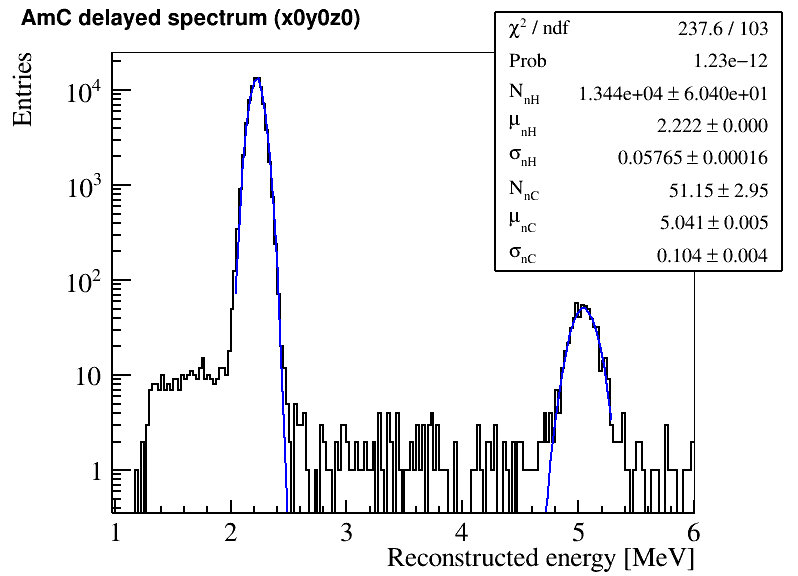
\includegraphics[width=0.5\linewidth]{4_efficiency/full_delayed_spec_AmC.png}
    \caption{Full delayed spectrum of AmC source.}
    \label{fig:full_delayed_spec_AmC}
\end{figure}


\subsubsection{Spill-in and spill-out effects}
If IBD reaction happen outside LS but near the edge of internal surface of acrylic vessel, the $\gamma$s from this electron-positron annihilation and the corresponding neutron may enter the LS region and contribute to the signal samples. However, since we only treat LS as the target volume, this contribution is not included in the prediction and should be considered separately. In this note, we call it spill-in effect.

Generally, IBD positron will deposite energy locally with only few millimeters displacement, while the $\gamma$s from this electron-positron annihilation will travel a few tens of cm. Besides, IBD neutrons take a few cm to be thermalized and the 2.2 MeV $\gamma$ from neutron capture travels a few tens of cm. Fortunately, since the edge of FV is far away from the internal surface of acrylic vessel ($\sim$ 1.2 m), these events can't reach the FV.
In short, spill-in effect is negligible, thanks to the tight FV cut.

For spill-out effect, $\gamma$s from the electron-positron annihilation and neutron go outside LS region. This effect has been included in the energy leakage effect.

These effects will be re-evaluated once the fine-tuning MC samples is ready.


\subsubsection{Summary}
Detector related systematic uncertainties for neutrino flux are summarized in \ref{tab:DetErr}.

\begin{table}[!htbp]
    \caption{Summary of detector related systematic uncertainties for neutrino flux in JUNO only analysis.}
    \label{tab:DetErr}
    \centering
    \footnotesize% fontsize
    \setlength{\tabcolsep}{4pt}% column separation
    \renewcommand{\arraystretch}{1.2}%row space 
    \begin{tabular}{lcc}
        \hline
         & Efficiency & Relative uncertainty \\ 
        \hline
        Proton number & - & 1\% \\
        Flasher cut & > 99.9\% & Negligible \\
        FV cut & 80.57\% & 1.6\% \\ 
        Prompt energy cut & 100\% & Negligible \\
        Delayed energy cut & 99.99\% & 0.1\% \\
        CD and WP muon veto & 95.55\% & Negligible \\
        Multiplicity cut & 97.36\% & Negligible \\
        Spallation neutron veto & 98.00\% & Negligible \\
        Coincidence time cut  & 96.80\% & 0.02\% \\
        Relative distance cut & 98.28\% & 0.10\% \\
        nH-nC ratio (neglect in first physics paper) & 99.32\% & 0.19\% \\
        \hline
        Total & 69.88\% & 1.89\% \\
        \hline
    \end{tabular}
\end{table}



\subsection{Energy response}

As shown in Fig.~\ref{fig:Energy_response_process}, the energy response of LS exhibits a non-linear dependence on the deposited energies of charged particles, primarily owing to ionization quenching and Cherenkov radiation effects. Additional non-linearity may arise during the PMT charge reconstruction process. Generally, dispersion and fluctuations occur in each stage of the energy response and detection process, collectively contributing to the overall energy resolution.

\begin{figure}[h]
    \centering
    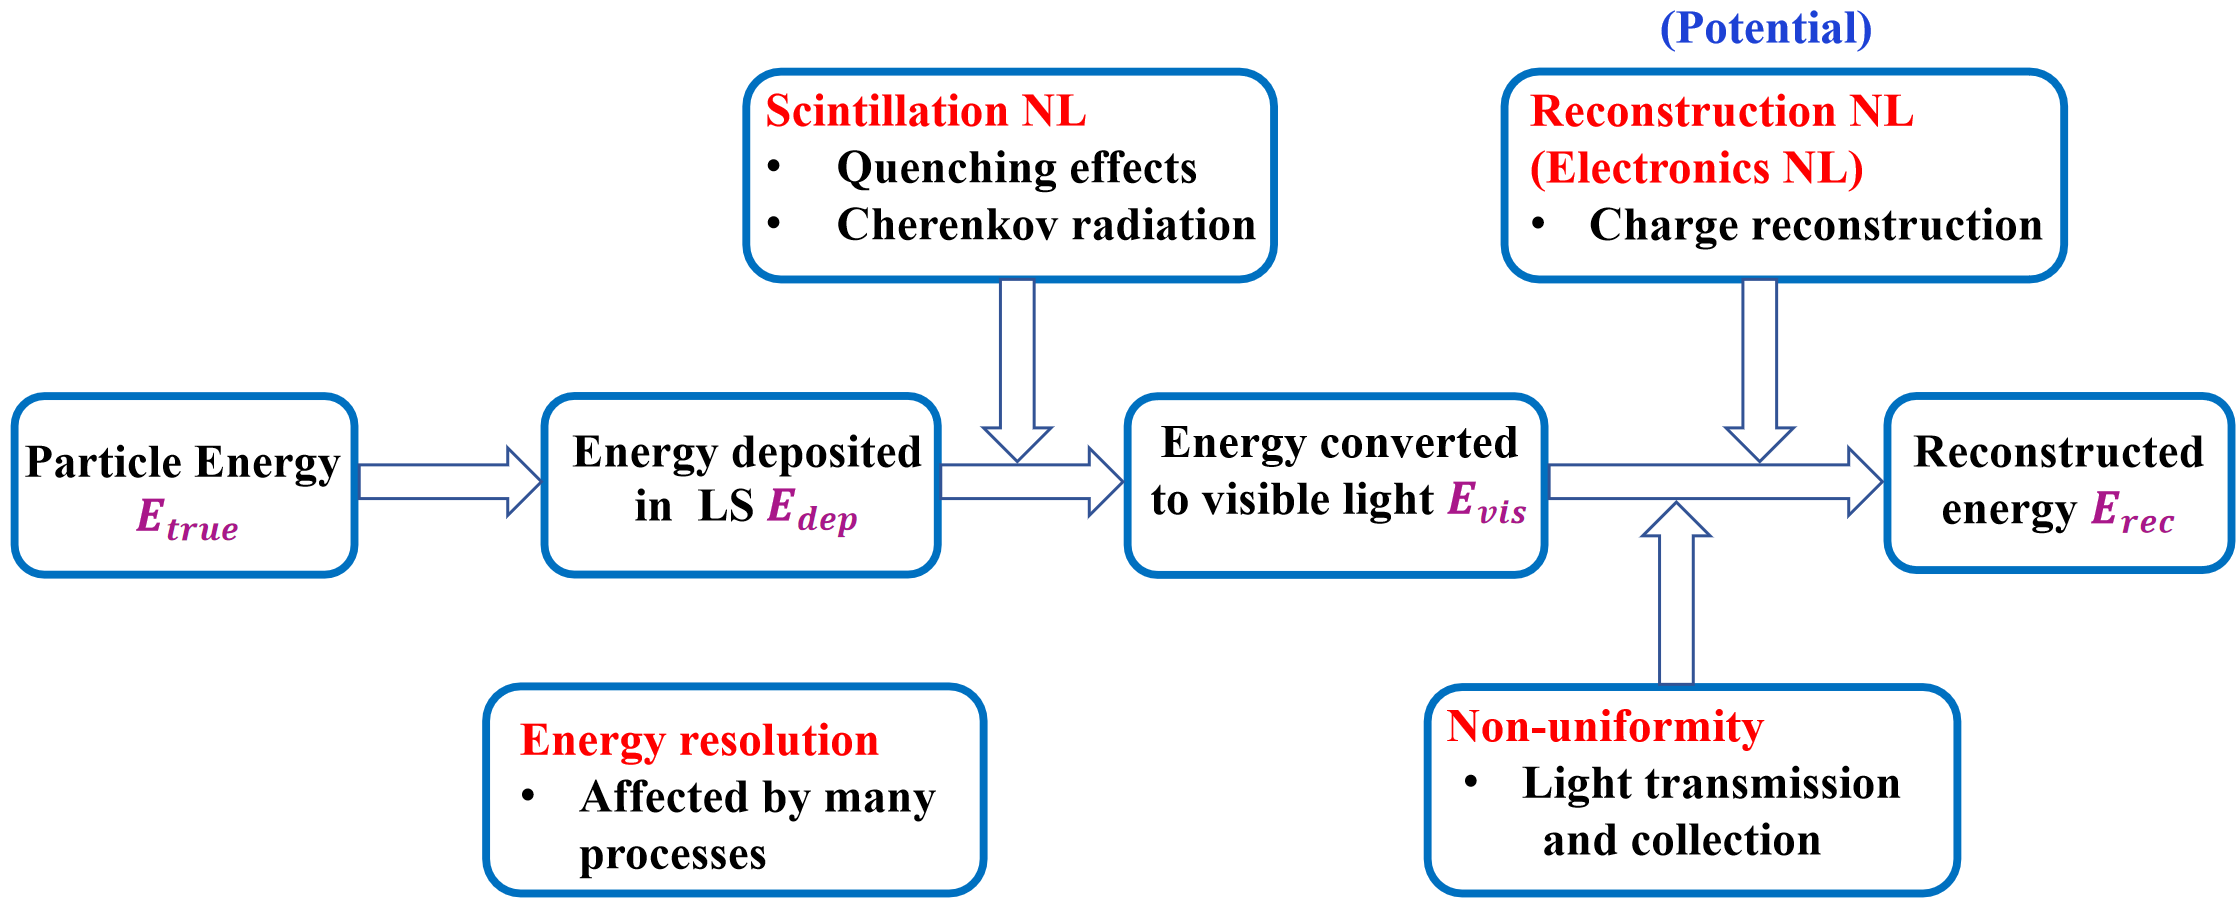
\includegraphics[width=0.9\linewidth]{4_efficiency/EnergyResponseProcess.png}
    \caption{The process of energy response.}
    \label{fig:Energy_response_process}
\end{figure}

\subsubsection{Calibration Source Selection}
\label{subsec:calibration_sources}

Table~\ref{tab:calibration_sources} summarizes the calibration sources utilized in the JUNO experiment for characterizing the energy response. These sources provide mono-energetic $\gamma$-rays and other characteristic signals across a wide energy range. The calibration strategy differs based on the source characteristics:
\begin{itemize}
    \item For \textbf{single-like events} (e.g., $\gamma$ sources like $^{137}\mathrm{Cs}$, $^{54}\mathrm{Mn}$), the event selection relies on the dynamic Fiducial Volume (FV) method described in Section~\ref{subsec:fv_selection}. Both the vertex reconstruction and energy estimation for these selections are based on the \textbf{P25C dataset}.
    \item For the AmC source, which requires identifying correlated prompt and delayed signals, an additional time coincidence selection is applied after the dynamic FV cuts to significantly reduce accidental backgrounds.
\end{itemize}

\begin{table}[h!]
\centering
\caption{Calibration sources used for energy response analysis in JUNO.}
\label{tab:calibration_sources}
\begin{tabular}{ccl}
\toprule
\textbf{Sources/Processes} & \textbf{Type} & \textbf{Radiation (MeV)} \\
\midrule
$^{137}\mathrm{Cs}$ & $\gamma$ & 0.662 \\
$^{54}\mathrm{Mn}$ & $\gamma$ & 0.835 \\
$^{60}\mathrm{Co}$ & $\gamma$ & 1.173 + 1.333 \\
$^{40}\mathrm{K}$ & $\gamma$ & 1.461 \\
$^{68}\mathrm{Ge}$ & $e^{+}$ & Annihilation 0.511 + 0.511 \\
$^{241}\mathrm{Am}$-$^{13}\mathrm{C}$ & $n, \gamma$ & $n + 6.13$ ($^{16}\mathrm{O}^{*}$) \\
$(n,\gamma)\mathrm{H}$ & $\gamma$ & 2.223 \\
$(n,\gamma)^{12}\mathrm{C}$ & $\gamma$ & 4.94 (68\%) or 3.68 + 1.26 (32\%) \\
\bottomrule
\end{tabular}
\end{table}

\paragraph{Dynamic Fiducial Volume Selection}
\label{subsec:fv_selection}

A data-driven approach is employed to define a run-dependent and source-position-dependent Fiducial Volume (FV) for each calibration run. This dynamic FV selection optimizes the signal-to-background ratio (S/B) by comparing the event distributions in both energy and spatial domains between the calibration data and a dedicated background run. A fundamental pre-selection requires all candidate events to pass a 5 ms muon veto to suppress backgrounds induced by cosmic-ray muons.

The dynamic FV selection algorithm proceeds sequentially through three dimensions:

\begin{enumerate}
    \item \textbf{Energy Region Selection:} The reconstructed energy spectrum ($E_{\mathrm{rec}}$) of the calibration run is compared with the background spectrum from one physic run. The relative difference, defined as $R_{\mathrm{diff}} = 100\% \times (N_{\mathrm{run}} - N_{\mathrm{bkg}})/N_{\mathrm{bkg}}$, is computed across energy bins. A threshold is set at the median of all $R_{\mathrm{diff}}$ bins, and a scanning algorithm identifies the contiguous energy region where $R_{\mathrm{diff}}$ consistently exceeds this threshold. This defines the optimal energy window for spatial selection in the following, typically centered around the expected $\gamma$-ray peak.
    \item \textbf{Radial ($\rho = \sqrt{x^2 + y^2}$) Constraint:} Using events within the selected energy range, the same $R_{\mathrm{diff}}$ method is applied to the radial distribution. The algorithm scans outward from $\rho = 0$ to find the radius $\rho_{\mathrm{max}}$ where $R_{\mathrm{diff}}$ drops below its mean value. This $\rho_{\mathrm{max}}$ defines the maximum radial extent of the FV for that run.
    \item \textbf{Longitudinal ($Z$) Constraint:} Events satisfying the previous energy and radial cuts are used to analyze the distribution of the reconstructed $Z$ coordinate relative to the expected source position $Z_{\mu}$. The $R_{\mathrm{diff}}$ thresholding yields $Z_{\mathrm{max}}$, the maximum allowed absolute deviation $|Z - Z_{\mu}|$ along the longitudinal axis.
\end{enumerate}

\begin{figure}[h!]
    \centering
    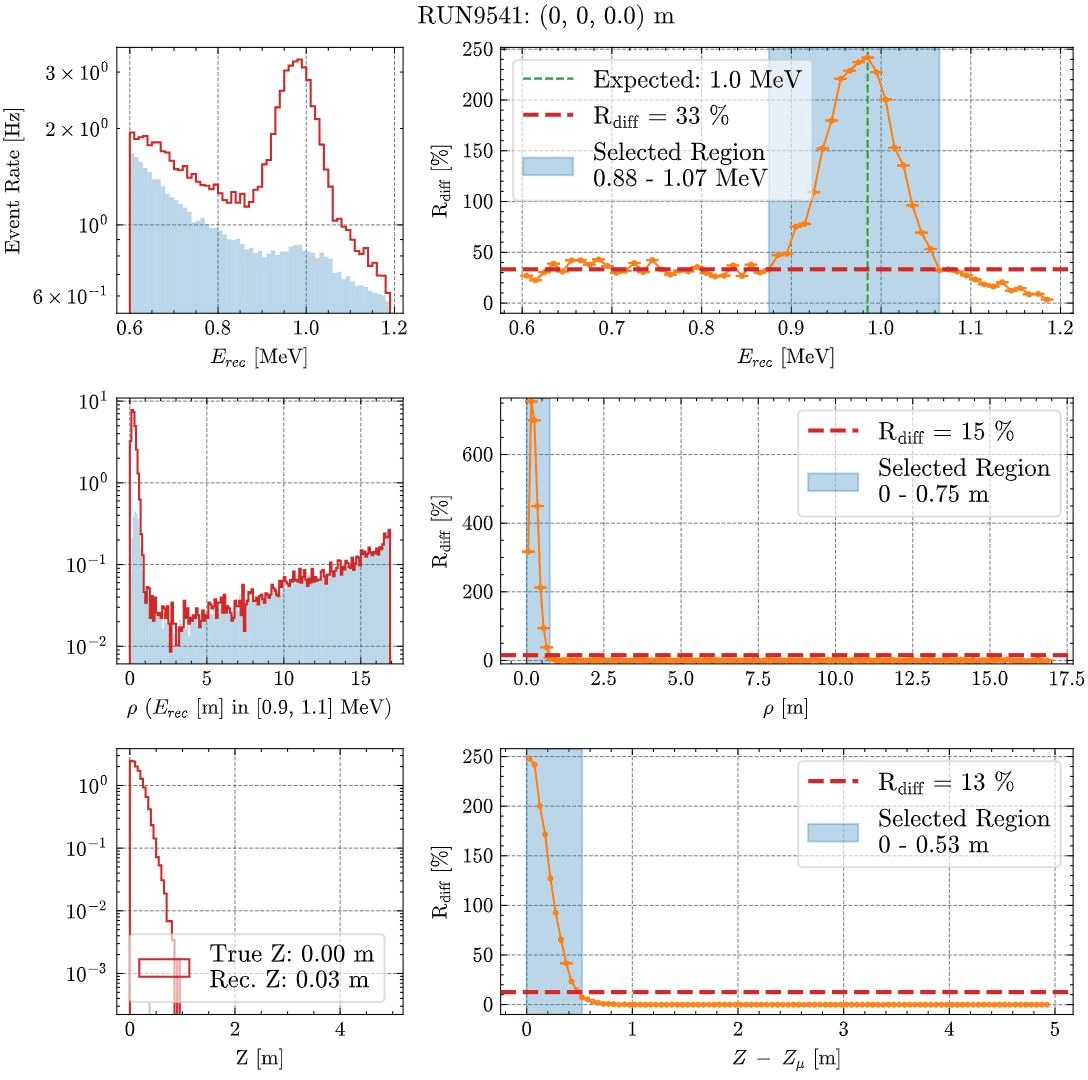
\includegraphics[width=0.8\textwidth]{4_efficiency/Ge68_FV_selection.png}
    \caption{Example of the dynamic Fiducial Volume selection for a central $^{68}$Ge run (RUN9541). \textbf{(Top)}: Energy spectra of the calibration run (red) and background (blue). \textbf{(Bottom)}: Relative difference $R_{\mathrm{diff}}$ with the selected energy region highlighted. The median $R_{\mathrm{diff}}$ threshold is shown as a red dashed line.}
    \label{fig:energy_selection}
\end{figure}

The final FV is defined by an elliptical cut based on the determined $\rho_{\mathrm{max}}$ and $Z_{\mathrm{max}}$. An event passes the FV cut if it satisfies the following condition:
$$
\sqrt{ \left(\frac{\rho}{\rho_{\mathrm{max}}}\right)^2 + \left(\frac{Z - Z_{\mu}}{Z_{\mathrm{max}}}\right)^2 } \leq 1
$$
where $\rho$ is the radial coordinate of the event and $Z$ is its longitudinal coordinate. The entire process is illustrated for a central $^{68}$Ge run in Fig.~\ref{fig:energy_selection}.

\paragraph{Correlation Selection for AmC Source}
\label{subsec:amc_selection}

Among all calibration sources, only the $^{241}\mathrm{Am}$-C (AmC) neutron source necessitates additional time correlation selection to identify the characteristic signature of neutron capture: a prompt signal from neutron reecoil or excitation, followed by a delayed $\gamma$-ray emission of neutron capture. The selection criteria are summarized in Table~\ref{tab:amc_cuts}. This method is applied after the dynamic FV selection described in Section~\ref{subsec:fv_selection} to further suppress accidental coincidences.

\begin{table}[h!]
\centering
\caption{Time correlation selection criteria for the AmC neutron source.}
\label{tab:amc_cuts}
\begin{tabular}{lll}
\toprule
\textbf{Parameter} & \textbf{Value} & \textbf{Description} \\
\midrule
$\Delta t_{\mathrm{max}}$ & 1 ms & Maximum time difference between prompt and delayed signals \\
$\mu$ veto & 5 ms & Muon veto window applied to all events \\
$E_{\mathrm{prompt}}$ & 0.3--12 MeV & Energy range for the prompt signal \\
$E_{\mathrm{delayed}}$ & 1.4--12 MeV & Energy range for the delayed signal \\
$d_{\mathrm{max}}$ & 5 m & Maximum spatial separation between prompt and delayed vertices \\
\bottomrule
\end{tabular}
\end{table}

The selection algorithm involves the following steps:

\begin{enumerate}
    \item \textbf{Initial Selection:} Events passing the dynamic FV cuts and within a broad energy range of $0.3 < E_{\mathrm{rec}} < 14$ MeV are selected as candidates.
    \item \textbf{Pair Finding:} All pairs of events within the same run occurring within a time window of $\Delta t < 1$ ms are identified. To minimize combinatorial background, only pairs consisting of exactly two events (one candidate prompt, one candidate delayed) are retained.
    \item \textbf{Energy and Distance Cuts:} Each pair must satisfy the energy conditions listed in Table~\ref{tab:amc_cuts} and have a spatial separation $d < 5$ m, ensuring the signals are spatially correlated.
\end{enumerate}

The time difference ($\Delta t$) distribution of the selected candidate pairs is then analyzed. It is fitted with a function of the form $f(\Delta t) = A e^{-\Delta t/\tau} + c$, where the decay constant $\tau$ corresponds to the neutron capture time. The fitted value of $\tau \approx 209$ $\mu$s is consistent with expectations for neutron thermalization and capture in the liquid scintillator, validating the selection efficiency. The results of this procedure, including the $\Delta t$ distribution fit and the correlation between prompt and delayed event energies, are shown in Fig.~\ref{fig:amc_selection}. After applying all selection criteria, the AmC event rate is approximately 70 Hz.

\begin{figure}[h!]
    \centering
    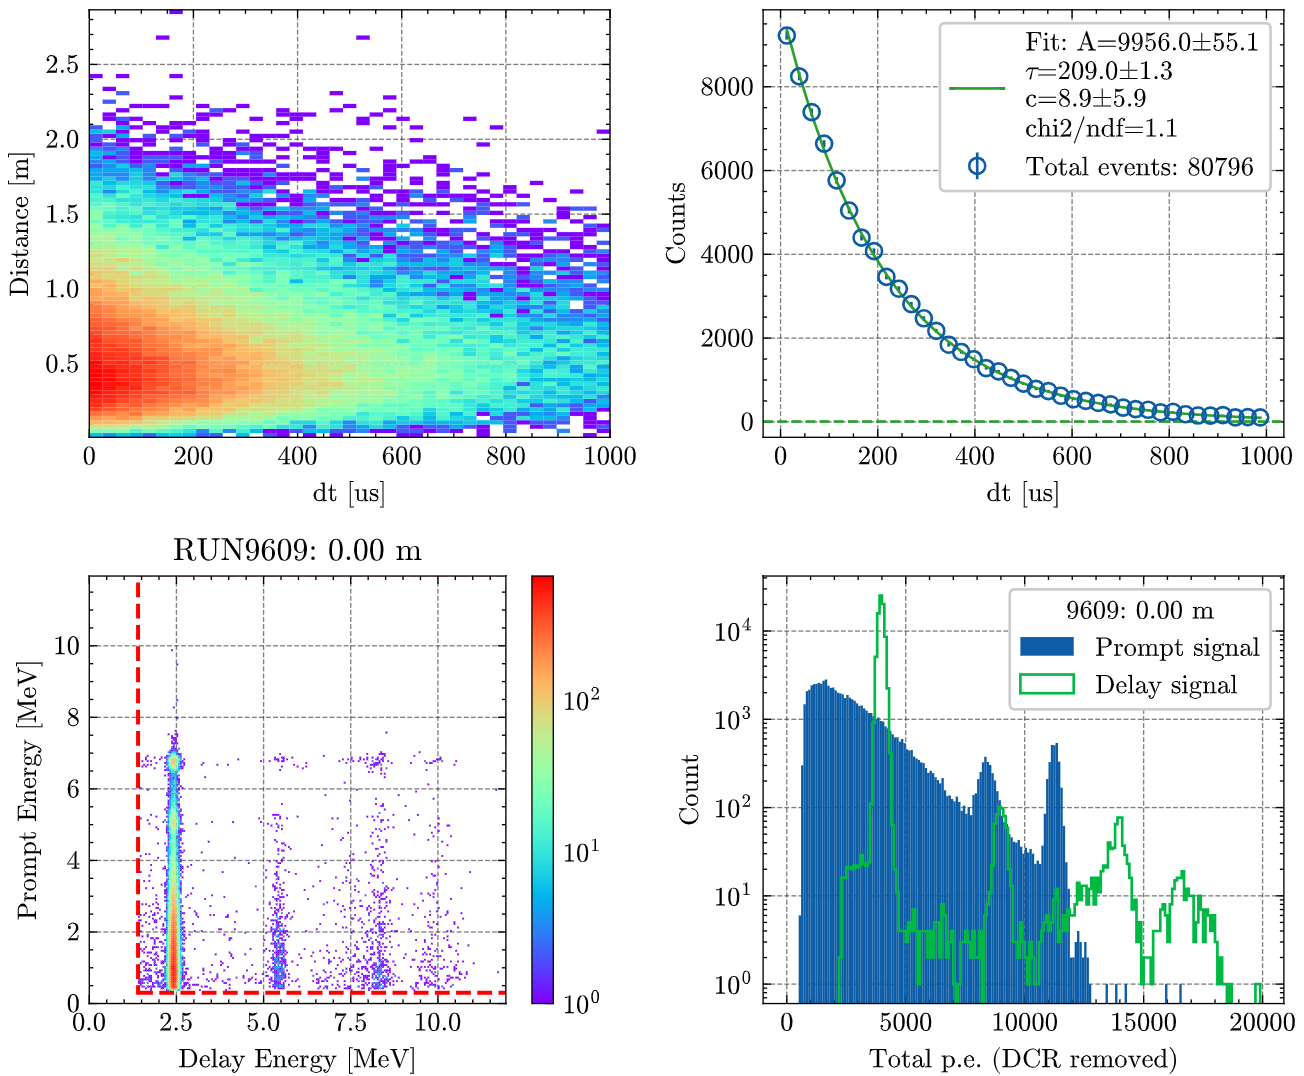
\includegraphics[width=0.9\textwidth]{4_efficiency/AmC_events.png}
    \caption{
        Comprehensive results of the time correlation selection for the AmC neutron source.
        \textbf{Top left}: The two-dimensional distribution of the time difference ($\Delta t$) versus spatial separation between candidate prompt and delayed events. The concentration of events at small $\Delta t$ and small distances is the characteristic signature of neutron capture.
        \textbf{Top right}: The projected $\Delta t$ distribution fitted with an exponential decay function plus a constant background. The extracted neutron capture time constant is approximately 200 $\mu$s, which is consistent with expectations for the liquid scintillator medium.
        \textbf{Bottom left}: The energy correlation plot between the prompt and delayed signals, revealing distinct clusters associated with different neutron interaction processes.
        \textbf{Bottom right}: The total PE energy spectra of the prompt (blue) and delayed (green) signals.
    }
    \label{fig:amc_selection}
\end{figure}

These clean samples provide crucial calibration points at several distinct energies and the energy spectrum is shown in (Fig.~\ref{fig:energy_spectrum}), which are essential for determining the energy scale and characterizing the non-linearity across the entire JUNO detector volume.
\begin{figure}[h!]
    \centering
    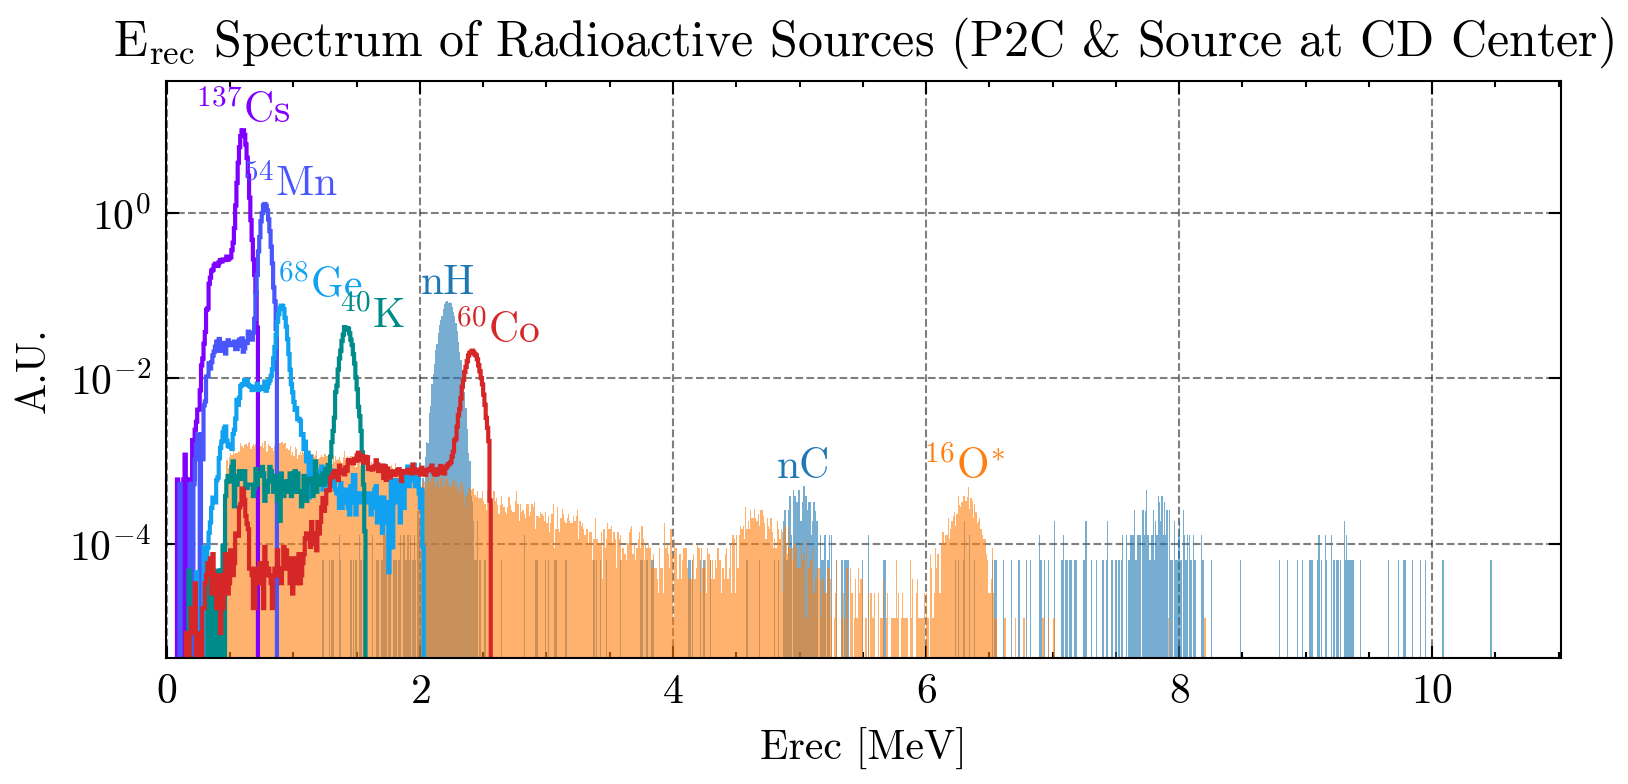
\includegraphics[width=0.9\textwidth]{4_efficiency/Energy_spectrum.png}
    \caption{The energy spectrum from various calibration sources after corresponding event selections}
    \label{fig:energy_spectrum}
\end{figure}

\subsubsection{Spallation Neutron Selection}
\label{subsec:spn_selec}

Spallation neutrons (SPN) are neutrons produced by hadronic showers induced by cosmic-ray muons as they traverse the detector.
%
These neutrons are characterized by the emission of a 2.223~MeV $\gamma$ ray when they are captured by hydrogen after thermalization, typically occurring on a timescale of several hundred microseconds following a CDmuon event.
%
Consequently, a clean sample of SPN can serve as a valuable monitor of temporal variations in the detector energy scale and can be used to estimate the energy scale uncertainty.
%
Furthermore, SPN provide an independent cross-check of the fiducial volume cut efficiency used in physics event selections such as IBD, and allow studies of energy non-linearity as a function of the event position within the detector.

To obtain a clean SPN enriched sample, we designed the selection criteria as 
follows (Fig.~\ref{fig:spn_selec}):

\begin{itemize}
    \item \textbf{Data set}: 
    /eos/juno/juno-reprod/ReProd25C/global\_trigger

    \item \textbf{Parent CDmuon}: OEC energy larger than 200~MeV;
    at least one water-pool muon within $(-2,\,2)\,\mu\text{s}$ of the parent CDmuon;
    no events with energy larger than $20$~MeV within $(-10,\,5)$~ms of the parent CDmuon.

    \item \textbf{In-window (SPN candidate)}: time interval to the parent CDmuon within $(100,\,2000)\,\mu\text{s}$;
    fiducial volume cut $R < 16.5$~m and $\lvert Z \rvert < 15.5$~m;
    afterpulse- and flasher-tag algorithms are applied to remove non-physical events.
    
    \item \textbf{Off-window (accidental background)}: the interval $(-2000,\,-5)\,\mu\text{s}$ before the parent CDmuon, used to characterize the accidental background in the in-window.
\end{itemize}

\begin{figure}[h!]
    \centering
    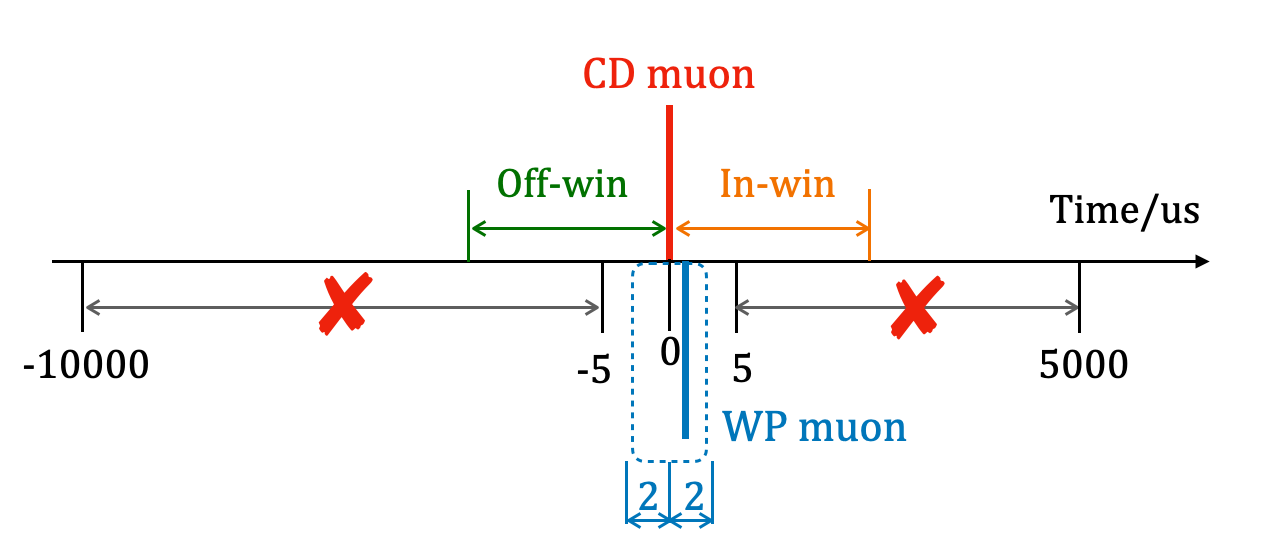
\includegraphics[width=0.9\textwidth]{4_efficiency/SPN_selection.png}
    \caption{Schematic illustration of the selection criteria for cosmogenic spallation neutron candidates.}
    \label{fig:spn_selec}
\end{figure}

In the energy spectrum and time distribution of the selected SPN enriched sample, the contributions from afterpulses and accidental backgrounds are modelled with polynomial and constant functions, respectively, while the SPN is described by a Gaussian distribution in energy and an exponential distribution in the time difference to the parent CDmuon.
%
The fit results are presented in Fig.~\ref{fig:spnFit}, yielding a reconstructed energy peak at 2.26~MeV and a characteristic time constant of 220~$\mu$s for the spallation neutrons captured by hydrogen.
%
Furthermore, by dividing the SPN enriched sample according to data-taking periods and detector spatial regions and performing the fits separately, the SPN sample provides a monitoring of the temporal variation of the detector energy scale (Fig.~\ref{fig:energy_correction_timeline}) as well as its dependence on the event position within the detector (Fig.~\ref{fig:energy_bias_uncertainty}).

\begin{figure}[h]
    \centering
    \begin{subfigure}[t]{0.45\textwidth}
        \centering
        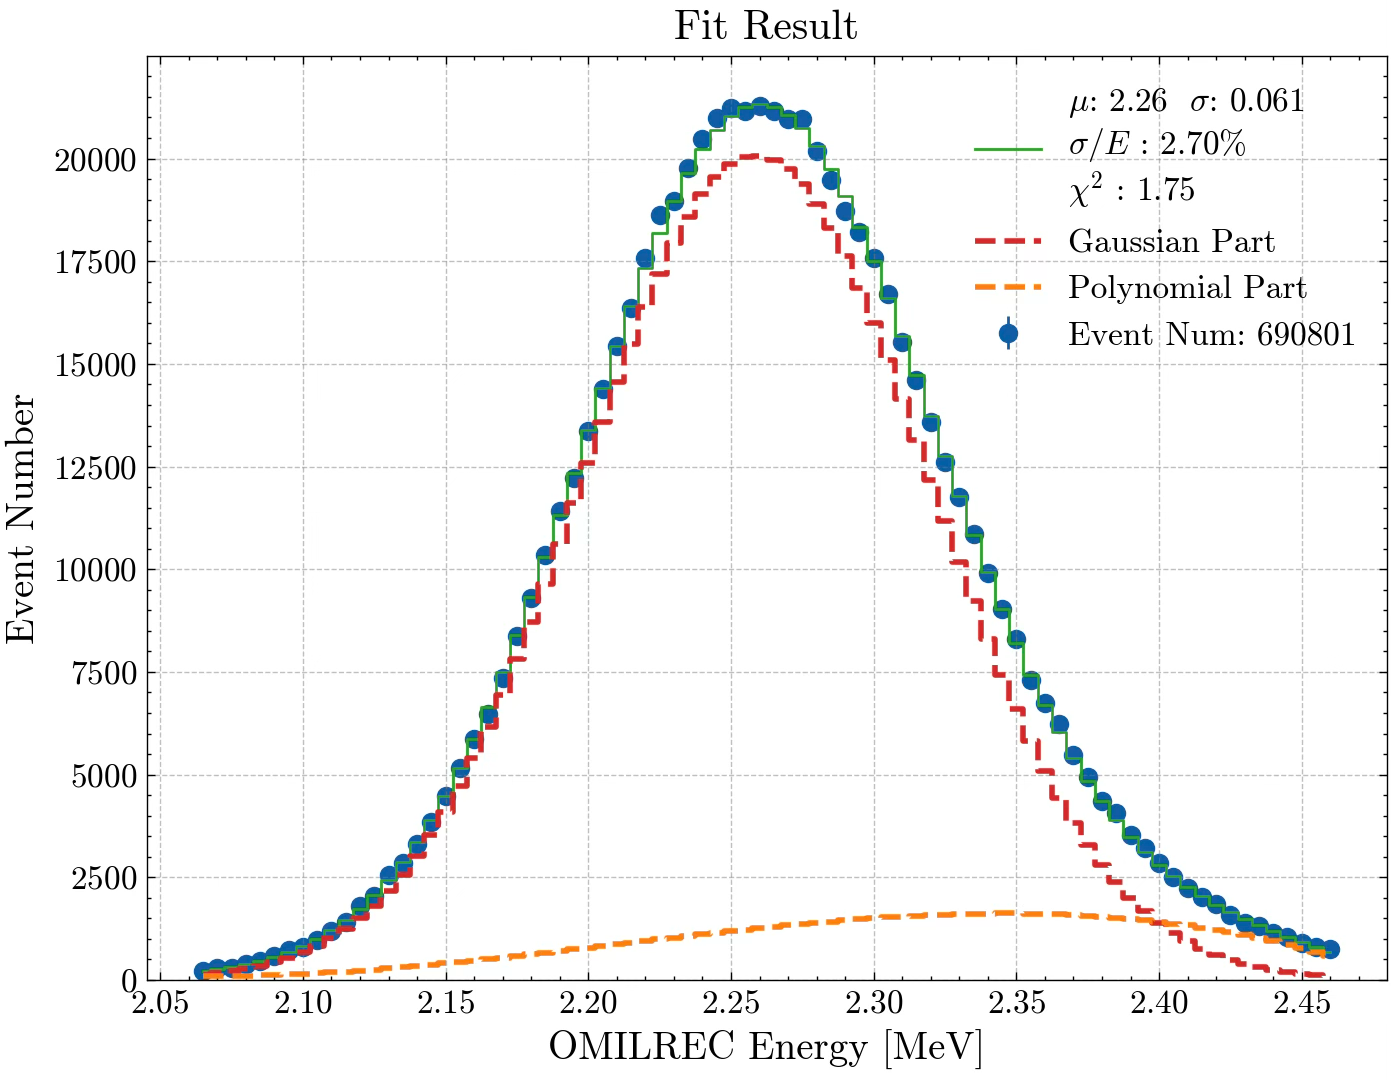
\includegraphics[width=\linewidth]{4_efficiency/SPN_energyFit.png}
        \caption{}
    \label{fig:spnEnergyFit}
    \end{subfigure}
    \hfill
    \begin{subfigure}[t]{0.45\textwidth}
        \centering
        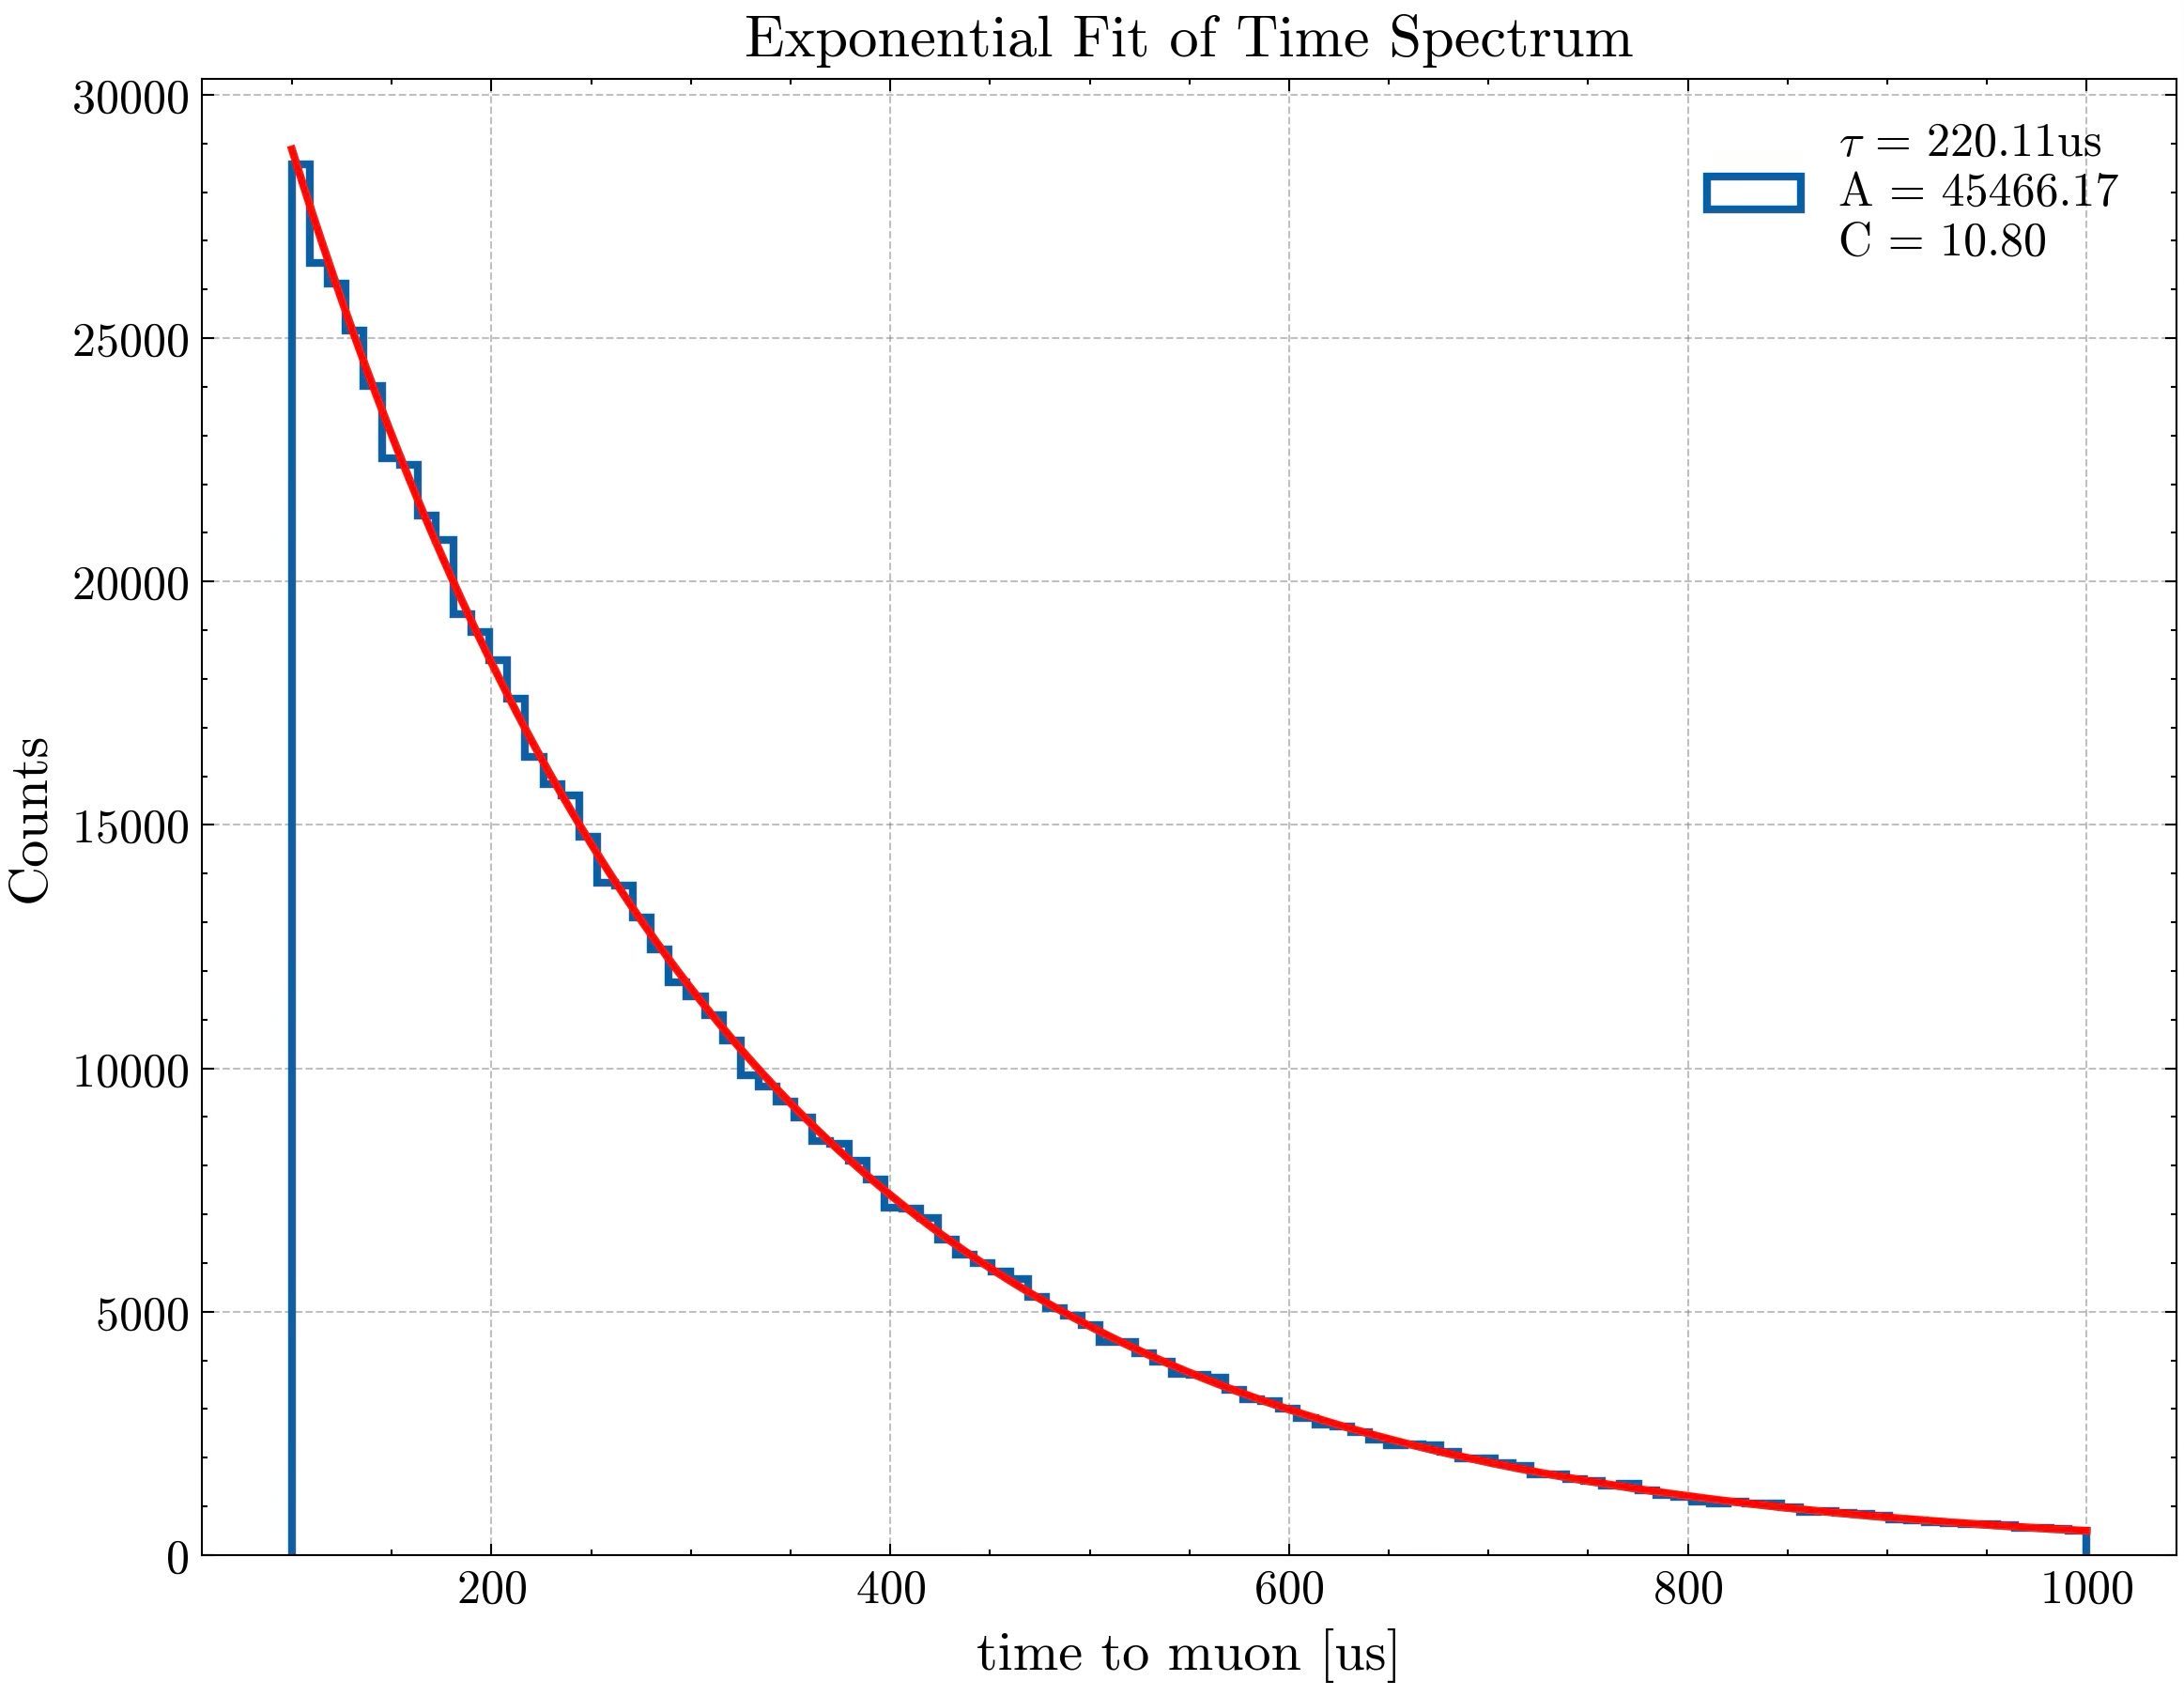
\includegraphics[width=\linewidth]{4_efficiency/SPN_dtFit.png}
        \caption{}
    \label{fig:spnDtFit}
    \end{subfigure}
    \caption{Fits to the energy spectrum~(a) and time distribution~(b) of the spallation neutron enriched sample, yielding a reconstructed energy peak at 2.26~MeV and a characteristic capture time of 220~$\mu$s for spallation neutrons captured by hydrogen.}
    \label{fig:spnFit}
\end{figure}


\subsubsection{Energy scale}
\label{subsec:energy_scale}

The accuracy of the energy reconstruction, known as the energy scale, is a critical input for precision physics measurements in JUNO, particularly for neutrino oscillation analyses. This section details the methodology for establishing, monitoring, and evaluating the systematic uncertainty of the energy scale using the P25C OMILRec dataset.

The energy scale is primarily monitored and corrected using two independent, high-statistics neutron samples: the AmC calibration source (via nH capture) and SPN. The AmC source provides precise, point-like calibrations, while the naturally occurring SPN events enable continuous, detector-wide monitoring. A significant energy drift was observed through P25C dataset. Following this shift, the method for energy drift correction transitioned from using the centrally deployed periodic AmC source to utilizing the SPN sample. The SPN-based correction accounts for the radial dependence of the energy response by calculating average correction factors within concentric spherical shells (e.g., \( R: [0.00, 10.39) \) m, \( [10.39, 13.10) \) m, etc.), providing a robust, day-by-day correction. The timeline of this transition and the evolution of the correction factors are illustrated in Fig.~\ref{fig:energy_correction_timeline}.

\begin{figure}[h!]
    \centering
    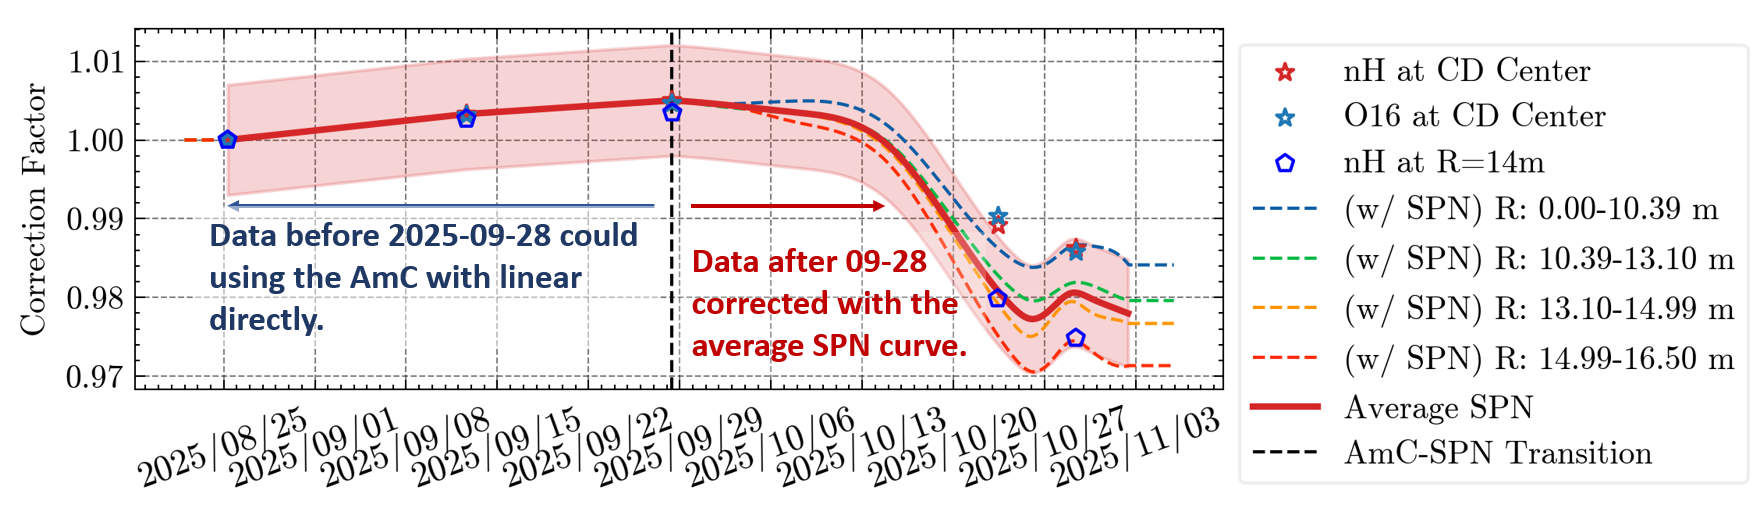
\includegraphics[width=0.9\linewidth]{4_efficiency/energy_scale_correction_timeline.png}
    \caption{
        Timeline of the energy scale correction factor. The correction methodology transitioned from using the central AmC source to a spallation neutron (SPN) based approach after September 28, 2025.
    }
    \label{fig:energy_correction_timeline}
\end{figure}

\paragraph{Assessment of Residual Temporal and Spatial Variations}

The systematic uncertainty of the energy scale is decomposed into residual temporal variation and residual detector non-uniformity. These components are constrained using full-detector samples: cosmogenic SPN and naturally occurring \( ^{214}\text{Po} \) and \( ^{210}\text{Po} \) isotopes from the \( ^{238}\text{U} \) and \( ^{232}\text{Th} \) decay chains.

The temporal stability is quantified by analyzing the daily average of the reconstructed energy \( E_{\text{rec}} \) for the \( ^{210}\text{Po} \) sample and SPN events. The observed root-mean-square (RMS) variation constrains the residual temporal instability to approximately \textbf{0.20\%}. 

To evaluate the spatial non-uniformity, the detector volume is partitioned into equal-volume boxes based on the statistics of available calibration samples. The partitioning scheme uses intervals in \( R^3 \), \( \cos\theta \), and \( \phi \) coordinates to ensure approximately equal statistics in each box. The reconstructed energy \( E_{\text{rec}} \) is calculated for each box using the \( ^{210}\text{Po} \) and SPN samples. The overall spatial variation is then determined by computing the RMS of the \( E_{\text{rec}} \) values across all boxes:

\[
\sigma_{\text{spatial}} = \sqrt{\frac{1}{N-1} \sum_{i=1}^{N} \left( E_{\text{rec}}^i - \langle E_{\text{rec}} \rangle \right)^2 }
\]

where \( N \) is the number of boxes, \( E_{\text{rec}}^i \) is the reconstructed energy in the \( i \)-th box, and \( \langle E_{\text{rec}} \rangle \) is the average reconstructed energy across all boxes. This analysis reveals a residual spatial non-uniformity of \textbf{0.45\%} within the fiducial volume. The consistency of the energy scale derived from these independent, full-volume samples validates that the temporal and spatial variations are well-understood and controlled. This analysis is summarized in Fig.~\ref{fig:energy_stability_uniformity}.

\begin{figure}[h!]
    \centering
    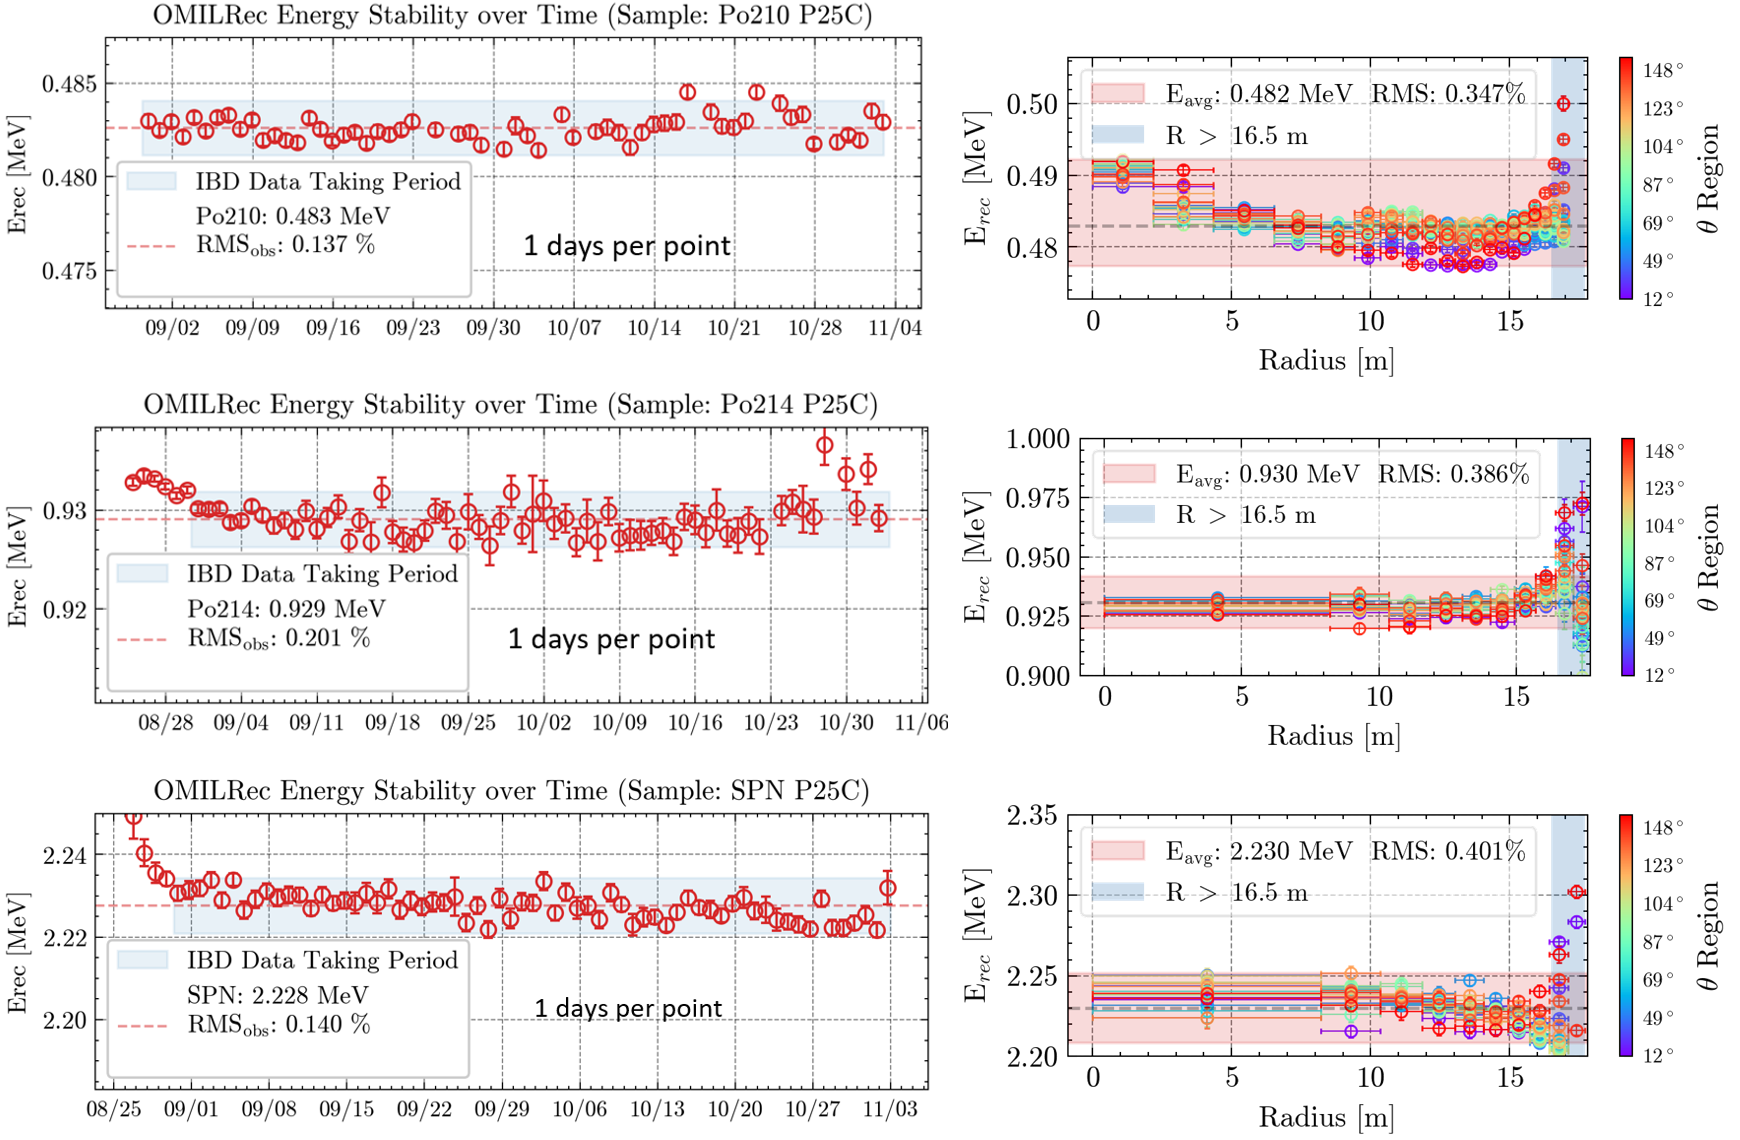
\includegraphics[width=\linewidth]{4_efficiency/energy_scale_stability_uniformity.png}
    \caption{
        Characterization of residual energy scale variations. \textbf{Left} Temporal stability of the reconstructed energy \( E_{\text{rec}} \) for the \( ^{210}\text{Po} \) sample and spallation neutrons. \textbf{Right} Spatial uniformity of \( E_{\text{rec}} \) as a function of detector radius \( R \) for the same samples in the left.
    }
    \label{fig:energy_stability_uniformity}
\end{figure}

\paragraph{Overall Systematic Uncertainty}

The overall systematic uncertainty on the energy scale is conservatively estimated by combining the residual temporal variation (\( \sigma_{\text{time}} \sim 0.20\% \)) and spatial non-uniformity (\( \sigma_{\text{spatial}} \sim 0.45\% \)) in quadrature:

\[
\sigma_{\text{total}} = \sqrt{ \sigma_{\text{time}}^2 + \sigma_{\text{spatial}}^2 }
\]

This yields a energy uncertainty of \textbf{0.50\%}. The robustness of this estimate is demonstrated by the excellent agreement among various independent calibration sources, as shown in Fig.~\ref{fig:energy_bias_uncertainty}. The energy bias \( (E_{\text{rec}} - E_0)/E_0 \) is plotted for neutrons from the AmC source, cosmogenic spallation, antineutrino candidates, \( \gamma \)-sources at fixed positions, and \( \alpha \)-decays from \( ^{214}\text{Po}/^{210}\text{Po} \). For the uniformly distributed \( ^{214}\text{Po} \) and \( ^{210}\text{Po} \) samples, which lack a defined central point, the average reconstructed energy \( \langle E \rangle \) over the detector volume is used as the reference value \( E_0 \). All measurements fall within the \textbf{±0.5\%} uncertainty band, confirming the reliability of the assigned systematic uncertainty for the energy scale in the energy region of interest for JUNO.

\begin{figure}[h!]
    \centering
    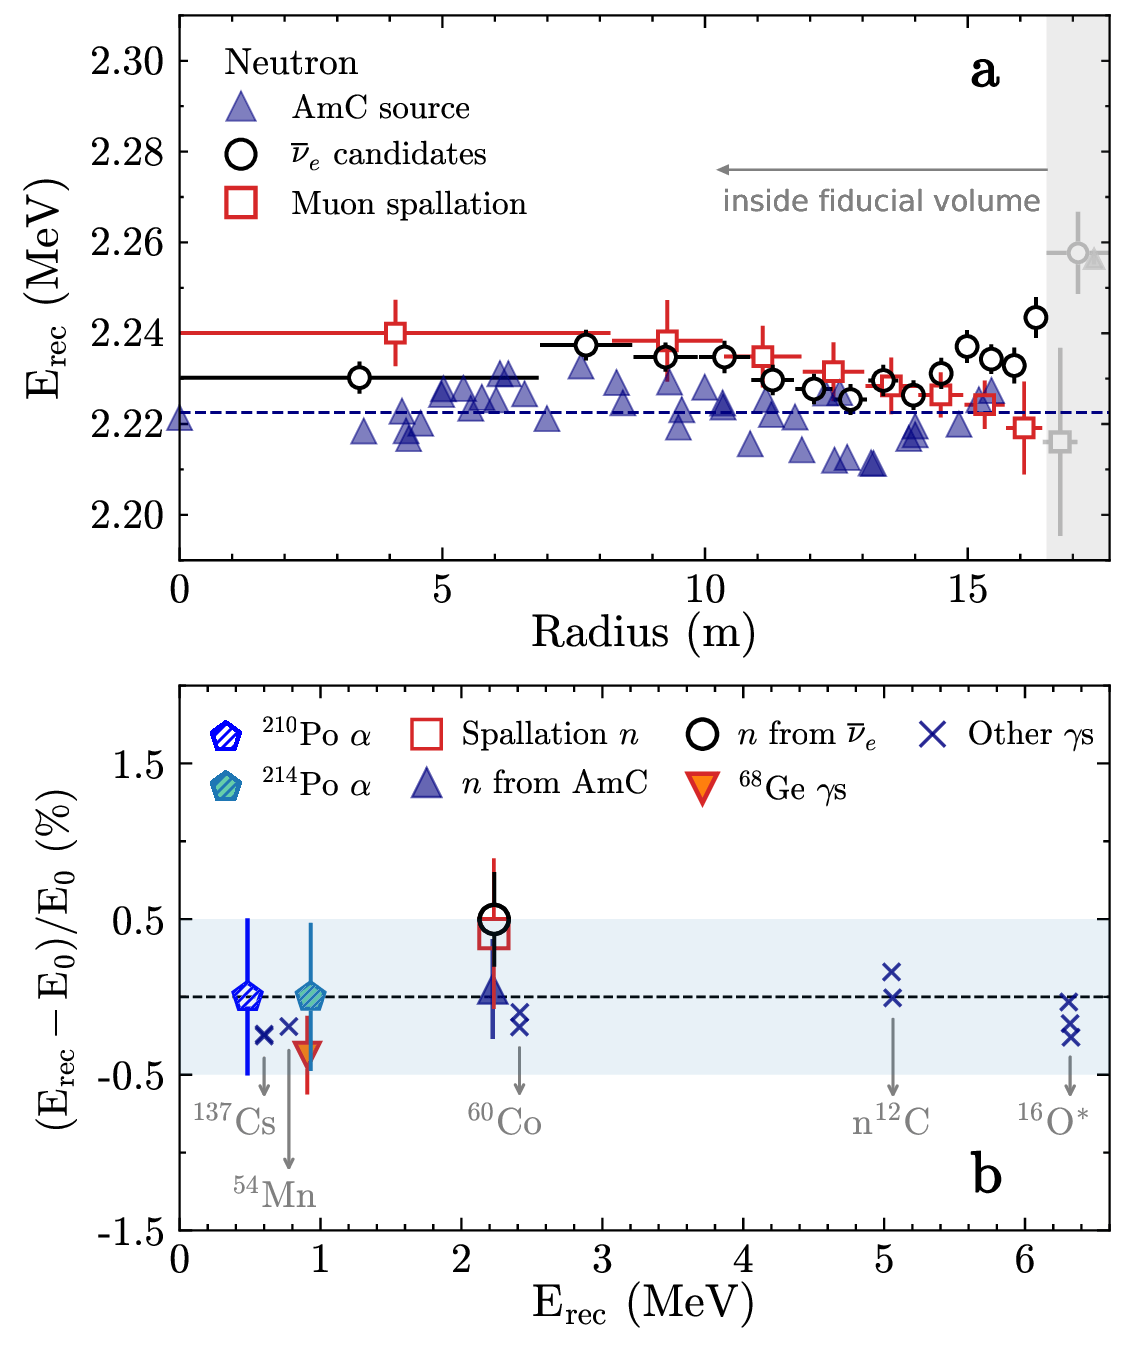
\includegraphics[width=0.8\linewidth]{4_efficiency/energy_bias_uncertainty.png}
    \caption{
        Residual energy bias and systematic uncertainty for the JUNO detector. The relative bias \( (E_{\text{rec}} - E_0)/E_0 \) is shown for various calibration sources, including neutrons (AmC, spallation, from IBD candidates), \( \gamma \)-sources, and \( \alpha \)-decays (\( ^{214}\text{Po}/^{210}\text{Po} \)). For the latter, the average reconstructed energy \( \langle E \rangle \) is used as \( E_0 \). Error bars include contributions from residual temporal and spatial variations. The shaded band represents the overall ±0.5\% systematic uncertainty assigned to the energy scale.
    }
    \label{fig:energy_bias_uncertainty}
\end{figure}

\subsubsection{Energy non-linearity}

This section introduces the modeling of the detector energy response to describe the relationship between the true energy of incident particles and the reconstructed energy. The modeling strategy mainly follows that of the Daya Bay experiment \cite{DayaBay:2019fje}. For JUNO, the non-linearity is predominantly governed by scintillation non-linearity; however, potential reconstruction-induced non-linearity require careful consideration. 

The Birks law is a semi-empirical method used to describe the quenching effect and was applied in this analysis. Several strategies are available for generating the quenching curves with different Birks'  coefficient ($k_B$), including a numerical integration method using $dE/dx$ data from ESTAR and a simulation-based approach utilizing Geant4. These two methods were respectively employed and compared. The Cherenkov contributions can also be modeled using various methods, including a Geant4-based simulation approach, a parametric function-based method, and an approach utilizing the Frank-Tamm formula. Considering the complex absorption and re-emission processes in the LS, only the shape of the Cherenkov contribution is used, and a free parameter $k_C$ is incorporated into the energy non-linearity model. Meanwhile, an additional free parameter $A$ is introduced to describe the absolute energy scale of scintillation non-linearity.


\begin{figure}[h]
  \centering
  \begin{subfigure}[t]{0.45\textwidth}
    \centering
    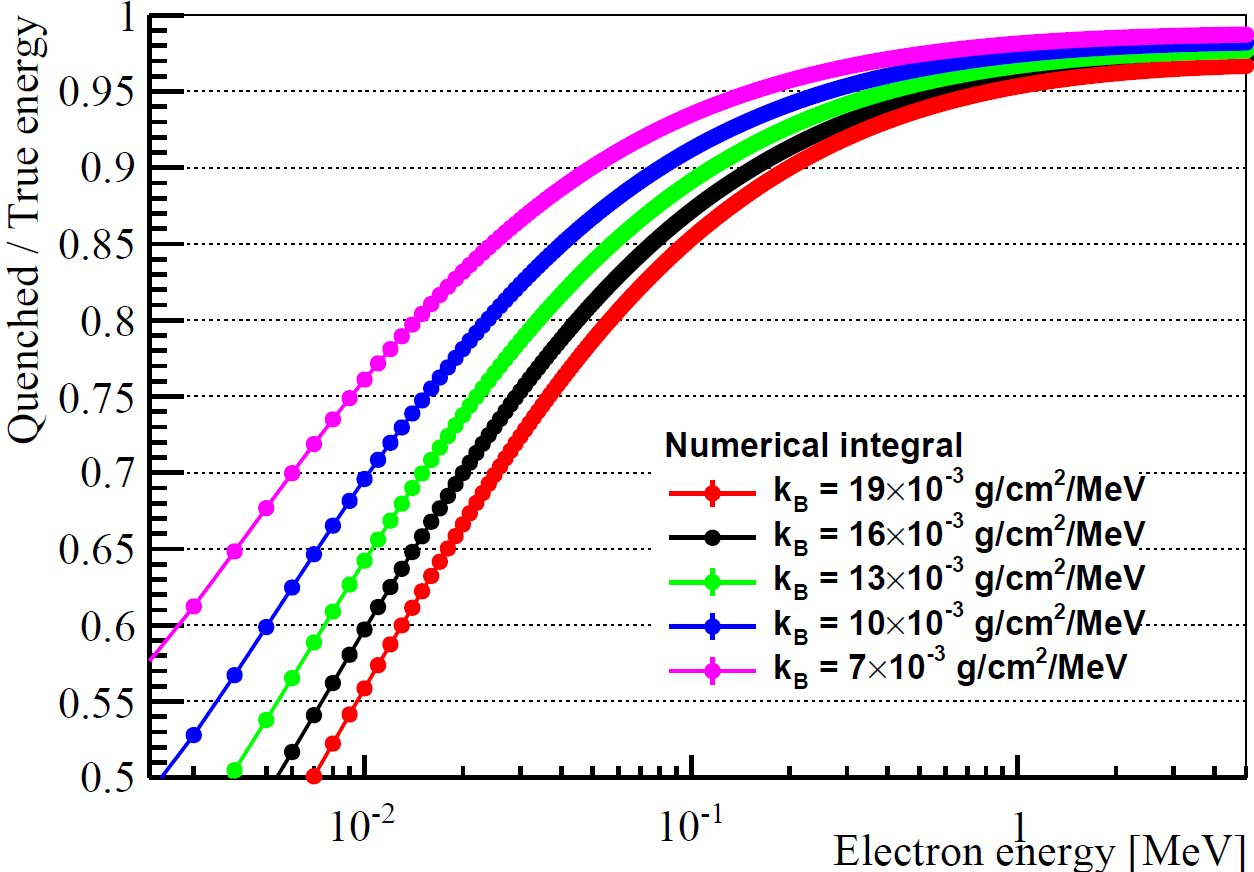
\includegraphics[width=\linewidth]{4_efficiency/quenchingCurves.png}
    \caption{}
    \label{fig:quenchingCurves}
  \end{subfigure}
  \hfill
  \begin{subfigure}[t]{0.45\textwidth}
    \centering
    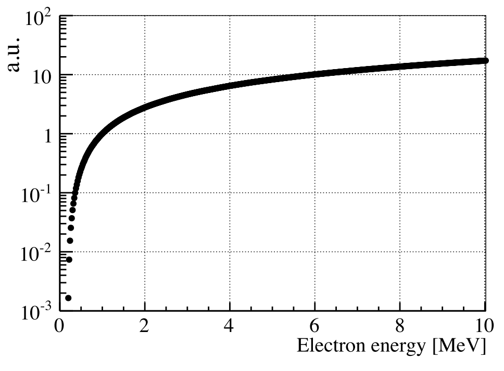
\includegraphics[width=\linewidth]{4_efficiency/CherenkovCurve.png}
    \caption{}
    \label{fig:CherenkovCurve}
  \end{subfigure}
  \caption{Examples of quenching curve and Cherenkov curve. (a) Relationship between deposited energy and visiable energy with different $k_B$ values, calculated with the numerical integration method. (b) The Cherenkov contribution to the $e^-$ kinetic energies, generated by Geant4 simulation and normalized at 1 MeV.}
\end{figure}

It is expected that minor deviations may occur in the COTI charge calculation under conditions involving multiple photoelectrons. According to current SPMT study \cite{spmt_doc_db}, the single-channel charge non-linearity of the LPMT remains below approximately 1\% over the range from 0 to 10 p.e. This non-linearity in charge reconstruction will be propagated to the energy measurement, referred to as the reconstruction non-linearity. In the analysis, it is assumed that the potential reconstruction non-linearity can be described by a gentle exponential function or a linear function, with all normalization points set at the nH peak position (2.223 MeV). For comparison, the case in which the reconstruction non-linearity is strictly zero—corresponding to perfect charge reconstruction—was also analyzed.

To constrain the model parameters and determine the energy nonlinear response, calibration is performed using data from multiple calibration sources positioned at the center of the detector and two kinds of continuous spectra from
high-purity samples ($\rm ^{12}B$ and $\rm ^{11}C$) of cosmogenic isotopes reconstructed in the FV. The former provides eight calibration points ($\rm ^{137}Cs$, $\rm ^{54}Mn$, $\rm ^{40}K$, $\rm ^{68}Ge$, $\rm nH$, $\rm ^{60}Co$, $\rm n^{12}C$, $\rm ^{16}O^{\star}$), which are detailed in Section~\ref{subsec:fv_selection}. The latter yields a continuous $\beta^{-}$ spectrum from $\rm ^{12}B$ decays and a $\beta^{+}$ spectrum from $\rm ^{11}C$ decays, with the visible energy increased by 2 $\times$ 511 keV due to annihilation gamma rays. Further details regarding the analysis of the calibration data can be found in \cite{sourceAna_doc_db} and \cite{spectrumAna_doc_db}.

All model parameters are determined through $\chi^{2}$ minimization to the combined calibration data. Considering that all the calibration sources are loaded at the center of the detector, the majority of the signals received by the PMTs are single photons. The corresponding charge reconstruction deviation can be ignored, so the reconstruction non-linearity was neglected when expecting their energy non-linearity. However, for the $^{12}$B sample which is uniformly distributed over the entire detector, the influence of potential reconstruction non-linearity was considered. The best-fit results to the mono-energetic peaks from gamma calibration sources and the continuous energy spectra from cosmogenic isotopes, as well as the predicted electron and positron non-linearities, are shown in Fig.~\ref{fig:Energy-nonlinearity}. An overall non-linearity uncertainty of 1\% is achieved for positron.

\begin{figure}[h!]
    \centering
    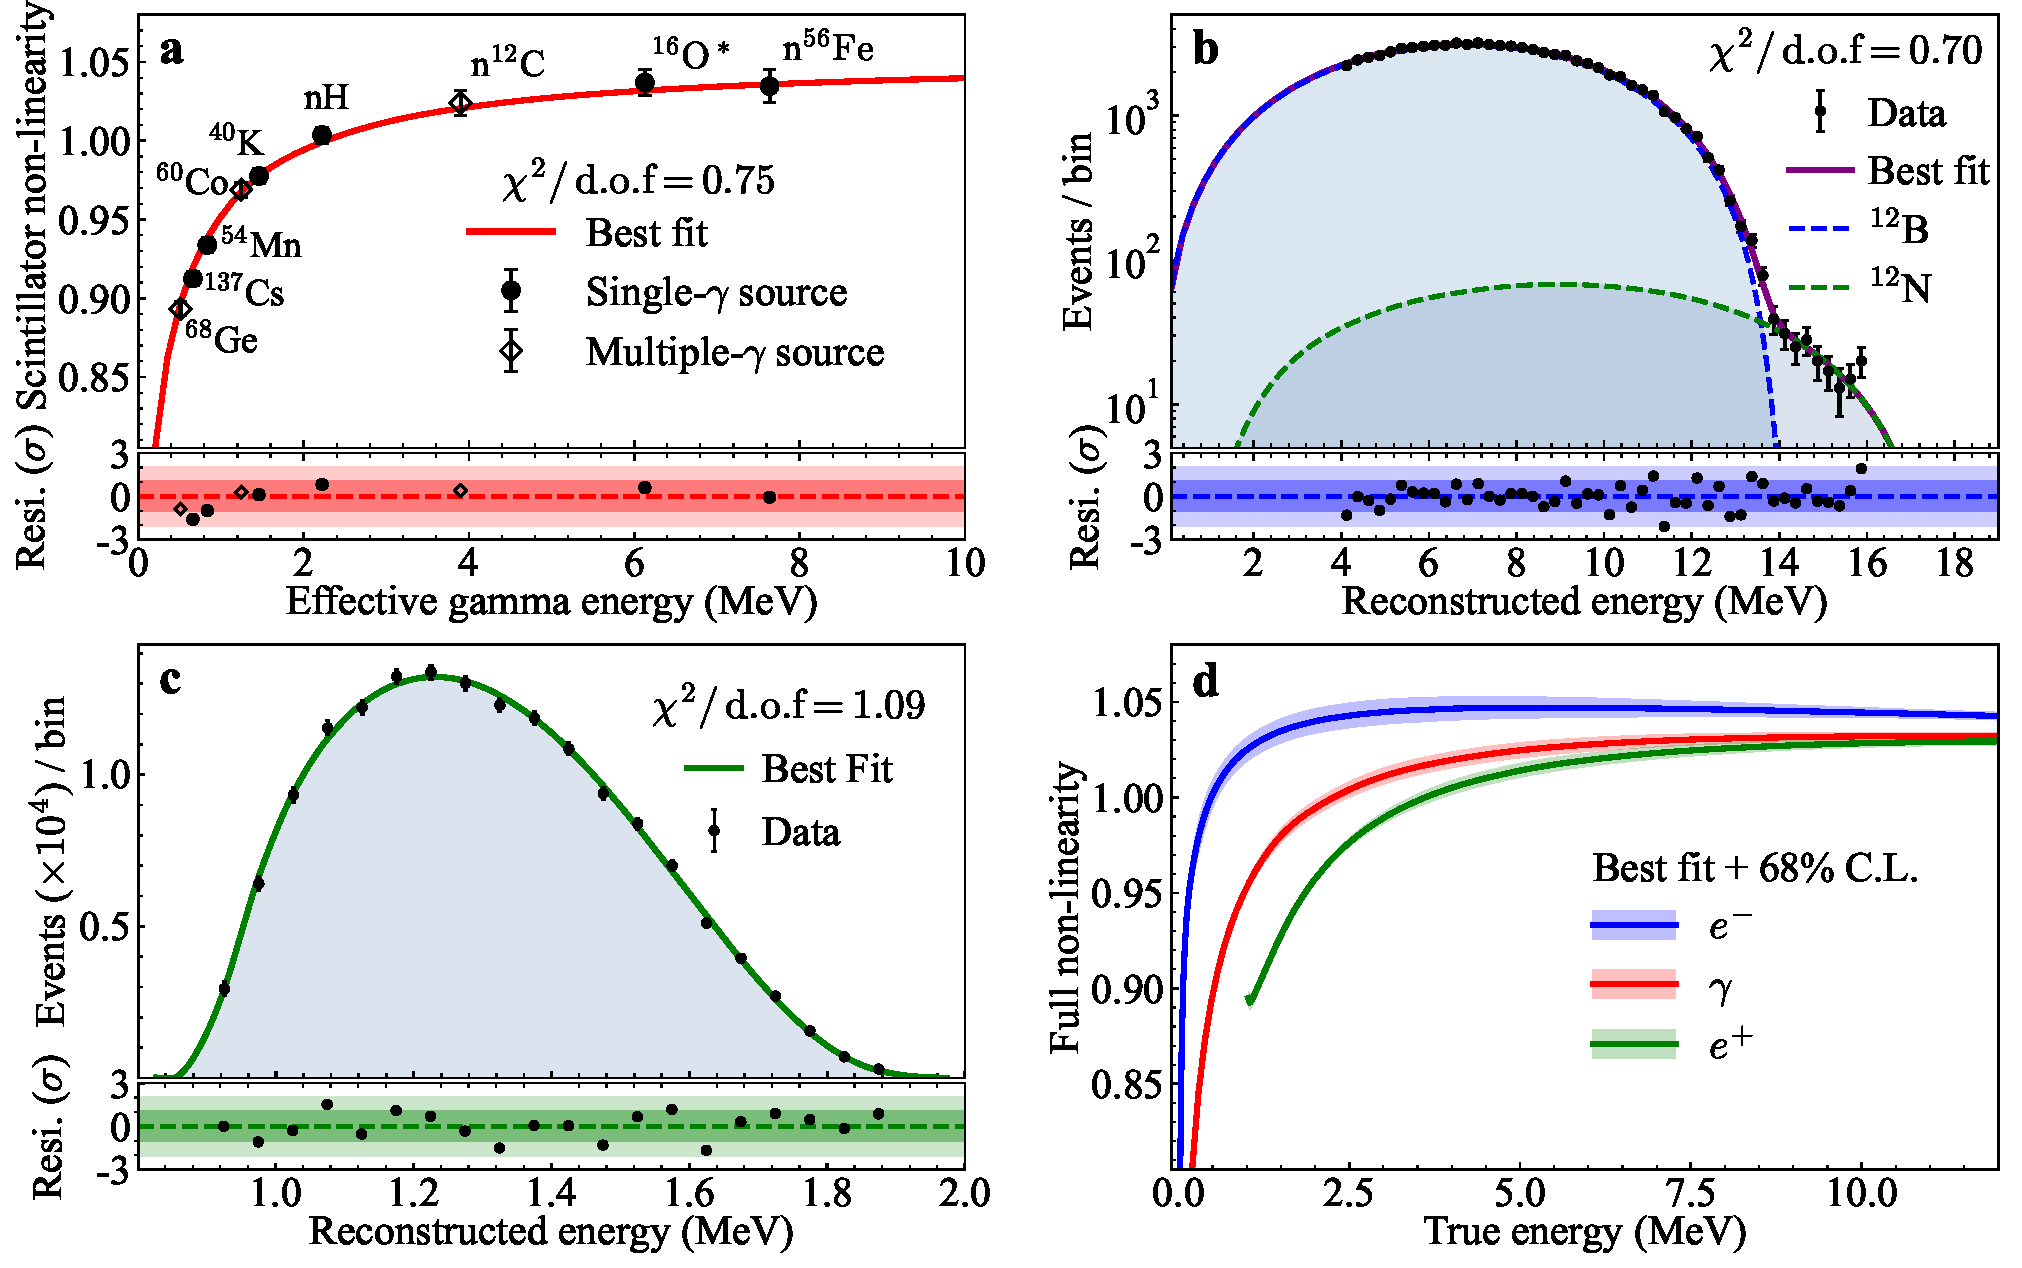
\includegraphics[width=0.9\linewidth]{4_efficiency/Energy-nonlinearity-groupA-Plots-fromYongbo-V15.pdf}
    \caption{Energy scale non-linearity calibration. \textbf{a}, Scintillator non-ninearity from $\gamma$ calibration sources deployed at the detector's center: single-$\gamma$ sources (solid circle), multiple-$\gamma$ sources (hollow rhombus), and the best-fit curve (red). \textbf{b}, Measured cosmogenic $^{12}$B $\beta^{-}$ spectrum (points) compared to prediction (blue line), with a best-fit $^{12}$N component (green dashed line)of 2.7\% identified via its high-energy shoulder. \textbf{c}, Measured $^{11}$C $\beta^{+}$ spectrum (points) and the best-fit model (green line). \textbf{d}, Non-linearity response model for electrons (blue), $\gamma$'s (red), and positrons (green).}
    \label{fig:Energy-nonlinearity}
\end{figure}


In addition, more tests and examinations were conducted, including the use of $^{12}$B samples from different selection strategies and different vertices, etc. A comparison of the non-linearity fits performed under two assumptions—no reconstruction non-linearity and the presence of reconstruction non-linearity (with pull parameter constrained)—shows that the resulting positron non-linearity curves do not differ significantly, with a discrepancy of approximately 0.2\% at 12 MeV. On the other hand, the de-excitation $\gamma$ from neutron absorption on Fe (n$^{56}$Fe) was used for additional validation. It was observed that including the n$^{56}$Fe calibration point in the fit leads to a change of less than 0.02\% in the positron non-linearity, as the $^{12}$B sample provides dominant constraints in the high-energy region. More details and comparison results can be found in \cite{ENL_check_doc_db}. 

\subsubsection{Energy resolution}
\label{subsubsection:EReso}
The energy resolution of the JUNO detector is a fundamental performance parameter that directly impacts the precision of neutrino oscillation measurements. Accurate characterization of the energy resolution is achieved through careful fitting of gamma source spectra. The fitting of gamma source energy spectra provides essential information about the detector's response function, statistical fluctuations, and systematic effects. The quality of these fits determines the reliability of the extracted resolution parameters, which are crucial inputs for the ABC model and subsequent physics analyses.


The energy resolution of the JUNO detector is parameterized using the ABC model, which describes the relative energy resolution $\sigma_E/E$ as a function of visible energy $E$:

\begin{equation}
\frac{\sigma_E}{E} = \sqrt{ \left(\frac{a}{\sqrt{E}}\right)^2 + b^2 + \left(\frac{c}{E}\right)^2 }
\label{eq:abc_model}
\end{equation}

where:
\begin{itemize}
    \item $a$ represents the statistical term related to photon statistics,
    \item $b$ is the constant term accounting for detector non-uniformity and systematic effects,
    \item $c$ is the noise term from electronics and dark noise.
\end{itemize}

This model captures the three dominant contributions to the energy resolution and provides a comprehensive description of the detector's energy response across the full energy range.

It is important to note that the energy resolution in JUNO exhibits particle dependence, as demonstrated in previous studies (e.g., Miao Yu et al.). The resolution for different particle types (electrons, positrons, gammas, etc.) can vary due to differences in energy deposition mechanisms, light yield, and ionization quenching effects. However, due to time constraints and the complexity of implementing particle-dependent resolution models, the current analysis for the P25C dataset utilizes the gamma resolution model as a conservative and standardized approach. This simplification provides a robust baseline for the energy resolution characterization while acknowledging that future analyses may incorporate particle-dependent corrections for improved precision.

\begin{figure}[h!]
    \centering
    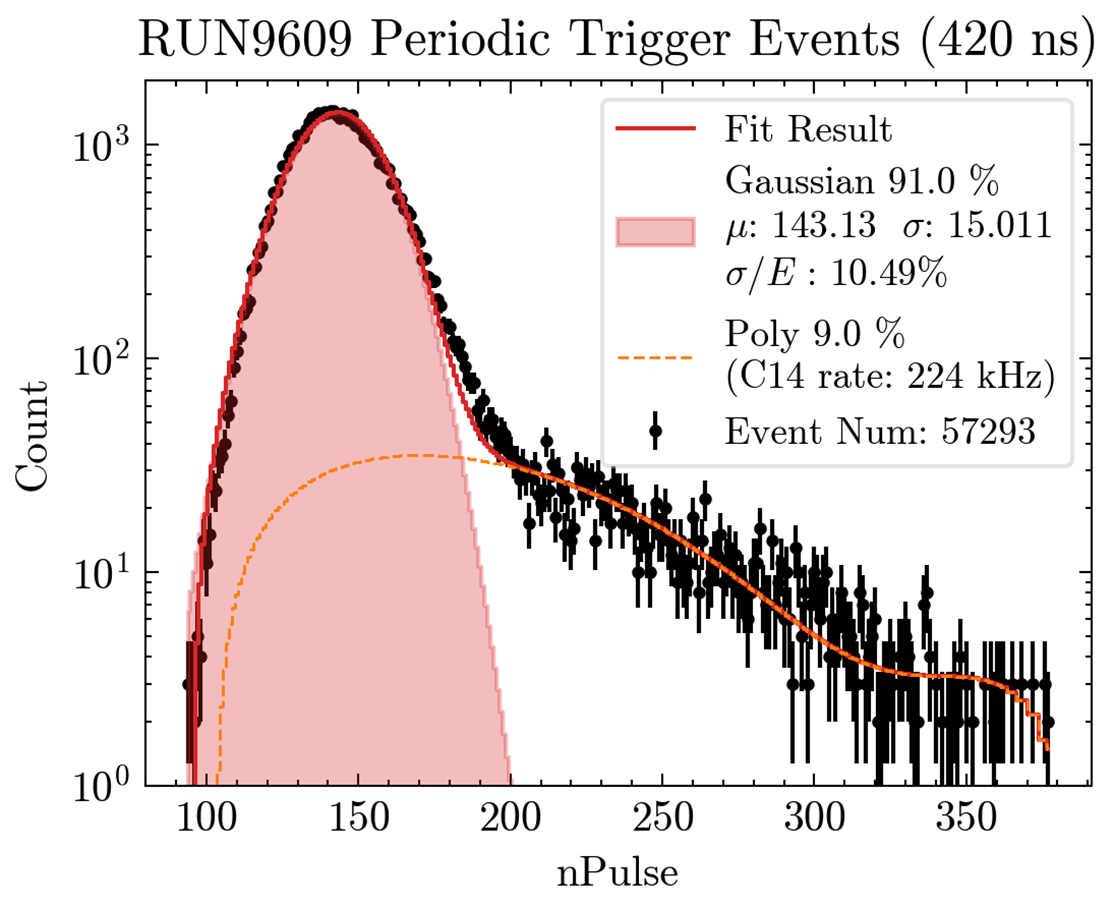
\includegraphics[width=0.8\textwidth]{4_efficiency/periodic_trigger_spectrum.png}
    \caption{Periodic trigger events nPulse spectrum of RUN9609 in 420 ns time window.}
    \label{fig:periodic_trigger}
\end{figure}

The presence of this $^{14}\text{C}$ pile-up tail distorts the energy spectrum of calibration sources. In an ideal, noise-free detector, the response to a mono-energetic gamma would be a near-Gaussian peak. However, the $^{14}\text{C}$ pile-up, by randomly adding low-energy deposits to physical events, broadens and asymmetrically skews this peak as shown in Fig.~\ref{fig:periodic_trigger}. Since a dedicated algorithm for identifying and subtracting $^{14}\text{C}$ pile-up events has not been applied to the P25C dataset, a critical question arises: how does the choice of fitting model (with or without explicit $^{14}\text{C}$ consideration) affect the extracted energy resolution? The following sections will detail and compare these two fitting strategies to quantify this effect.


\paragraph{Fitting Models Without $^{14}\text{C}$ Consideration}
For the majority of calibration sources, two simplified fitting approaches are employed when ignoring $^{14}\text{C}$ effects:
\begin{enumerate}
    \item \textbf{Purely Empirical Formula}: A Gaussian peak plus polynomial background, as shown for $^{137}\text{Cs}$ in Fig.~\ref{fig:cs137_wo_c14}(left).
    \item \textbf{MC-Based Spectrum Fitting for $^{68}$Ge}: Using MC simulations to generate template spectra for fitting, as shown in in Fig.~\ref{fig:cs137_wo_c14}(right).
\end{enumerate}


\begin{figure}[h!]
    \centering
    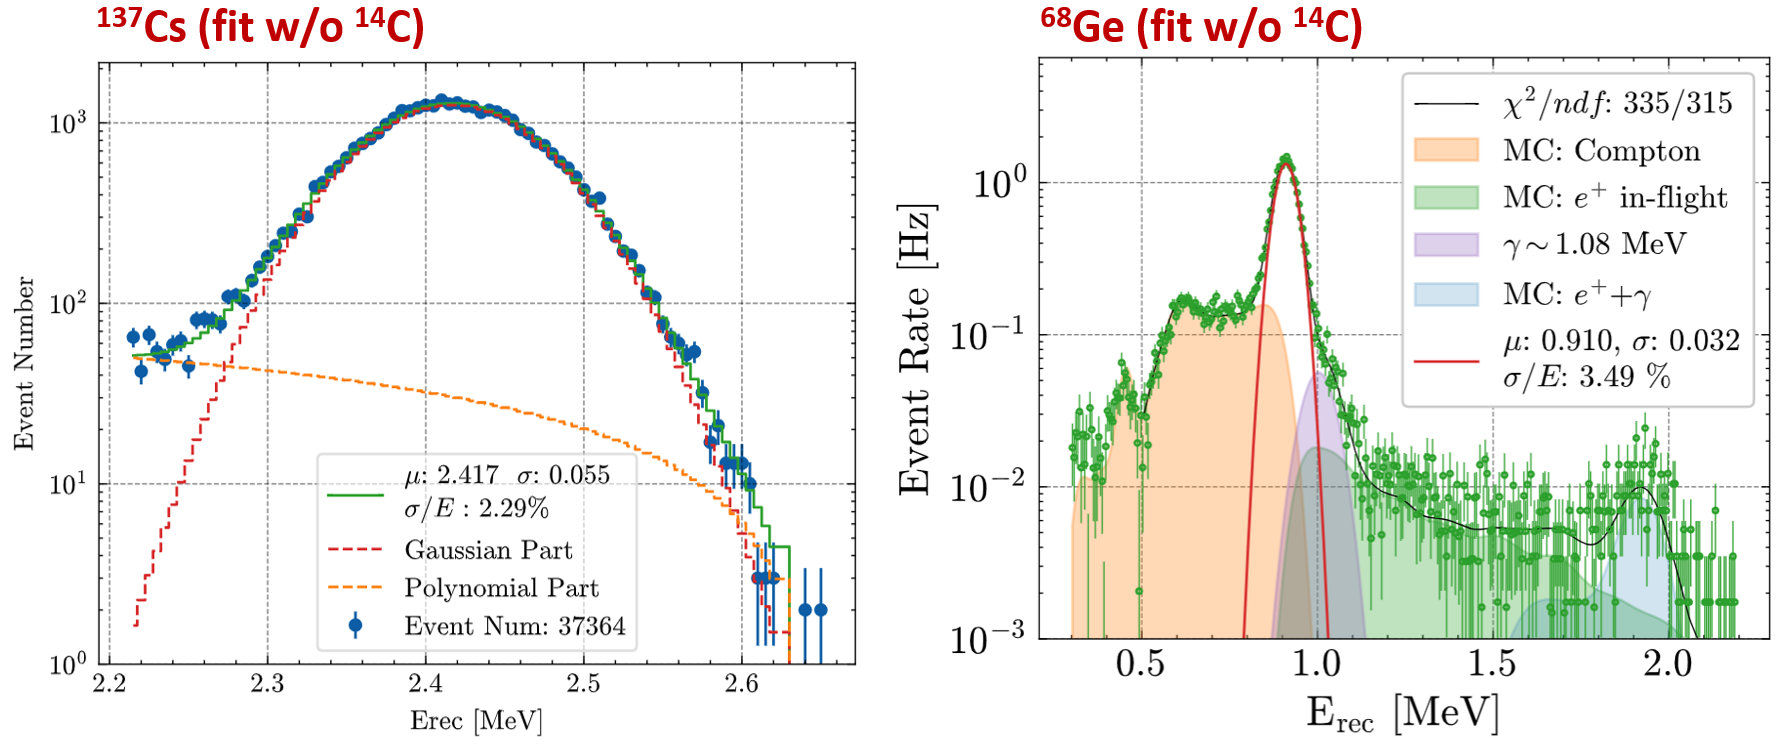
\includegraphics[width=0.8\textwidth]{4_efficiency/Cs137_wo_c14.png}
    \caption{\textbf{Left}: $^{60}\text{Co}$ energy spectrum fitted without $^{14}\text{C}$ consideration. The 2.506 MeV $\gamma$ peak is modeled as a Gaussian plus a polynomial background.\textbf{Right}: MC-based fitting result of $^{68}$Ge}
    \label{fig:cs137_wo_c14}
\end{figure}

\paragraph{Fitting Model with $^{14}\text{C}$ Consideration}
To properly account for $^{14}\text{C}$ effects, we developed a comprehensive fitting framework that incorporates probability weights. The complete model for $^{137}$Cs is formulated as:

\begin{equation}
\begin{aligned}
F_{\text{total}}(E) = & (1 - p - p^{2}) \cdot \left[ A_{\text{FEP}} \cdot f_{\text{FEP}}(E; \mu, \sigma) + A_{\text{Compton}} \cdot f_{\text{Compton}}(E) \right] \\
& + p \cdot F_{\text{1-pile}}(E) + p^{2} \cdot F_{\text{2-pile}}(E)
\end{aligned}
\label{eq:enhanced_fitting_model}
\end{equation}

where:
\begin{itemize}
    \item $A_{\text{FEP}}$ and $A_{\text{Compton}}$ are the amplitude factors for the full-energy peak and Compton background components,
    \item $f_{\text{FEP}}(E; \mu, \sigma)$ is the full-energy peak distribution, modeled as a Gaussian,
    \item $f_{\text{Compton}}(E)$ is the Compton background distribution obtained from MC simulations,
    \item $p$ represent the probabilities of $^{14}\text{C}$ pile-up events, with $(1 - p - p^{2})$ being the probability of no pile-up,
    \item $F_{\text{1-pile}}(E)$ and $F_{\text{2-pile}}(E)$ are the single and double pile-up distributions.
\end{itemize}

The pile-up terms are explicitly defined as convolution operations:

\begin{equation}
\begin{aligned}
F_{\text{1-pile}}(E) &= \left[ A_{\text{FEP}} \cdot f_{\text{FEP}}(E; \mu, \sigma) + A_{\text{Compton}} \cdot f_{\text{Compton}}(E) \right] \ast f_{\text{$^{14}$C}}(E) \\
F_{\text{2-pile}}(E) &= F_{\text{1-pile}}(E) \ast f_{\text{$^{14}$C}}(E)
\end{aligned}
\label{eq:convolution_definitions}
\end{equation}



where $\ast$ denotes the convolution operation, and $f_{\text{$^{14}$C}}(E)$ represents the $^{14}\text{C}$ Qedep energy spectrum. The energy resolution term $\sigma(E)$ used in the Gaussian components is determined by the ABC model mentioned before. Fig.~\ref{fig:with_c14_fits} shows representative fitting results with $^{14}\text{C}$ consideration for multiple sources.

\begin{figure}[h!]
    \centering
    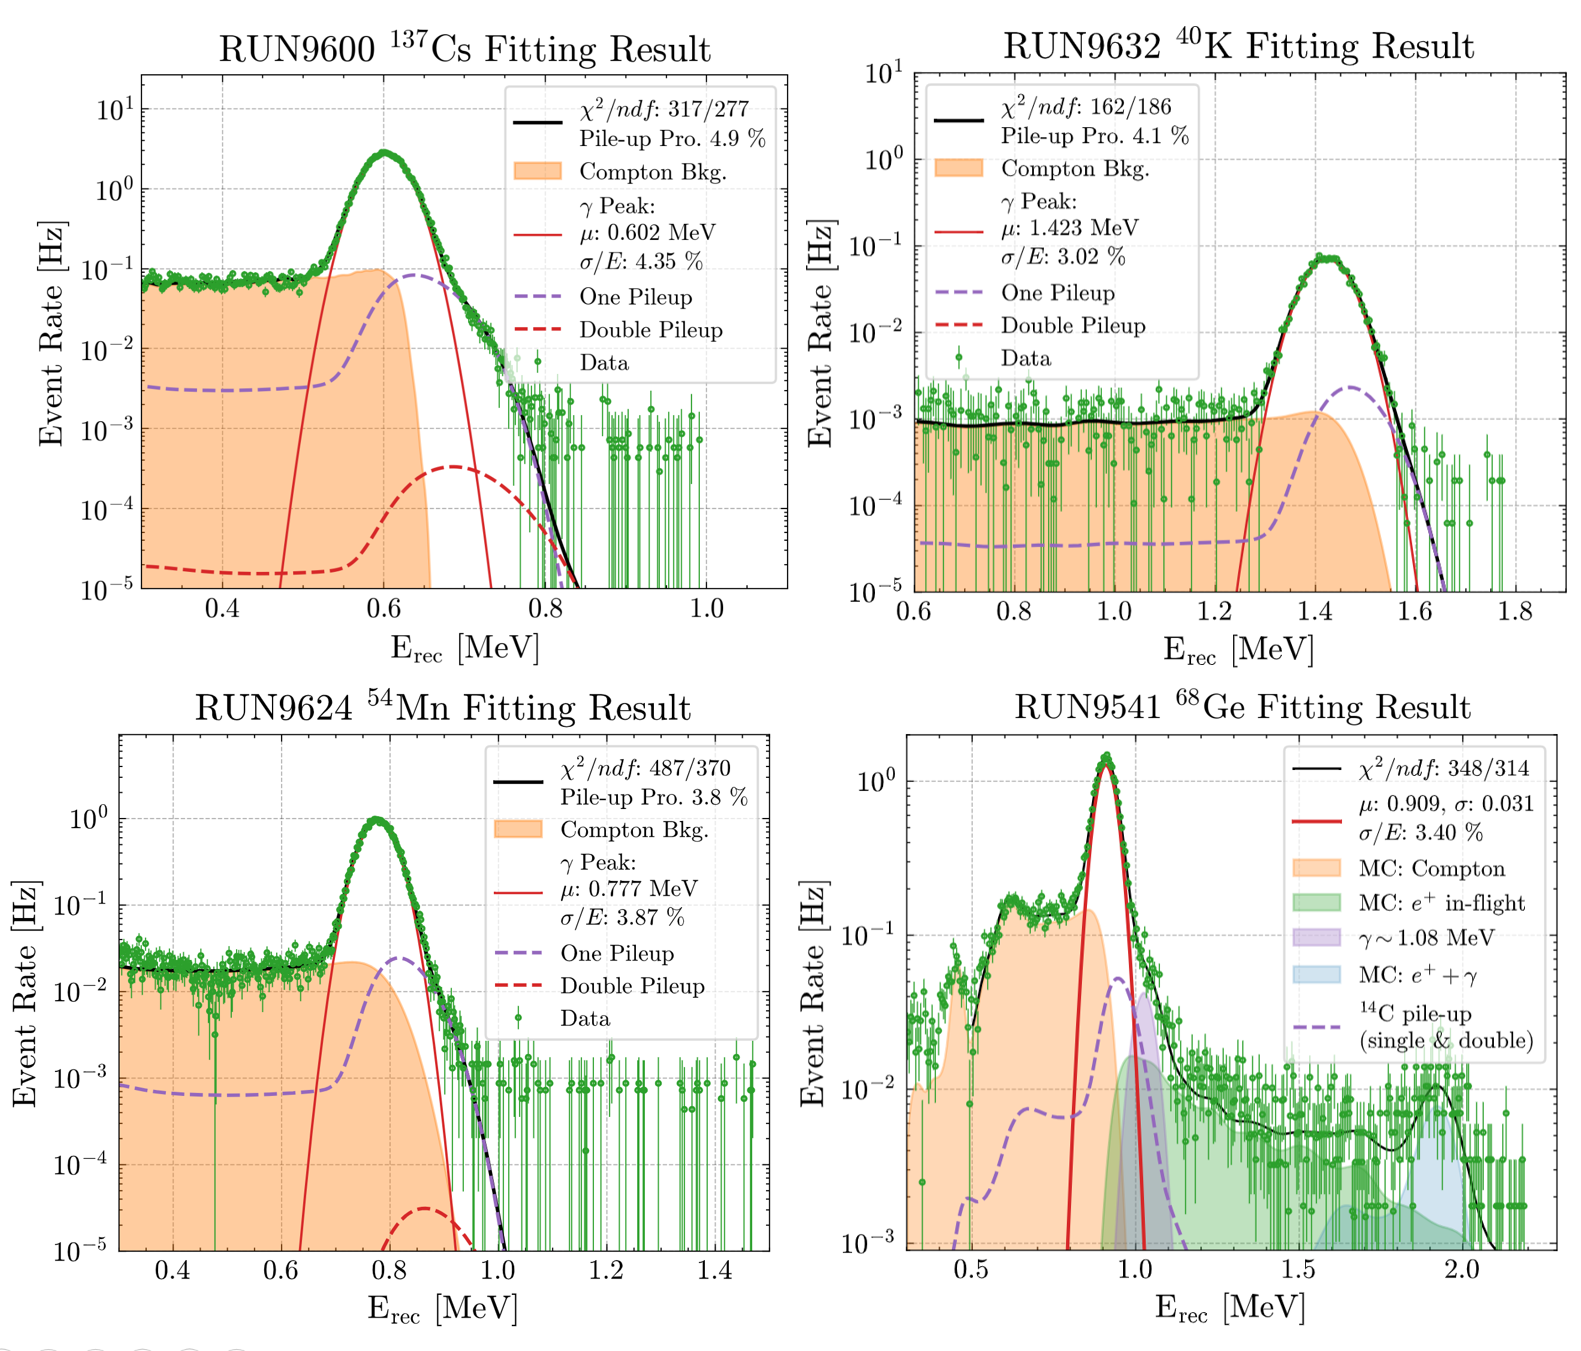
\includegraphics[width=\textwidth]{4_efficiency/with_c14_fits.png}
    \caption{Energy spectrum fits with $^{14}\text{C}$ consideration for multiple sources. Each panel shows: data (green points), total fit (black line), Compton background (orange fill), full-energy peak (red line), single pile-up (purple dashed), and double pile-up (red dashed). Fitting parameters including $\chi^2/\text{ndf}$ and pile-up probability are indicated.}
    \label{fig:with_c14_fits}
\end{figure}

Table~\ref{tab:resolution_results} summarizes the energy resolution measurements for all calibration sources, comparing results obtained with and without $^{14}\text{C}$ consideration in the fitting model.

\begin{table}[h!]
\centering
\caption{Energy resolution measurements for calibration sources. Results are shown for both fitting approaches: without $^{14}\text{C}$ consideration (w/o $^{14}\text{C}$) and with $^{14}\text{C}$ consideration (w/ $^{14}\text{C}$).}
\label{tab:resolution_results}
\resizebox{\linewidth}{!}{
\begin{tabular}{lcccc}
\toprule
\textbf{Source} & \textbf{$\text{E}_{\text{rec}}$ (w/o $^{14}\text{C}$) [MeV]} & \textbf{$\text{E}_{\text{rec}}$ (w/ $^{14}\text{C}$) [MeV]} & \textbf{Resolution (w/o $^{14}\text{C}$) [\%]} & \textbf{Resolution (w/ $^{14}\text{C}$) [\%]} \\
\midrule
$^{137}\text{Cs}$ & 0.602 & 0.602 & 4.449 & 4.349 \\
$^{54}\text{Mn}$ & 0.777 & 0.777 & 3.958 & 3.870 \\
$^{68}\text{Ge}$ & 0.910 & 0.909 & 3.526 & 3.404 \\
$^{40}\text{K}$ & 1.423 & 1.423 & 3.066 & 3.019 \\
nH & 2.221 & 2.221 & 2.576 & --- \\
$^{60}\text{Co}$ & 2.417 & 2.419 & 2.291 & 2.306 \\
nC & 5.028 & 5.028 & 2.219 & --- \\
$^{16}\text{O}$ & 6.303 & 6.303 & 1.642 & --- \\
\bottomrule
\end{tabular}
}
\end{table}

\begin{itemize}
    \item The reconstructed energies are remarkably consistent between the two fitting approaches, with differences typically less than 0.1\%.
    \item Energy resolution shows the expected improvement with increasing energy, from 4.449\% at 0.602 MeV ($^{137}\text{Cs}$) to 1.642\% at 6.303 MeV ($^{16}\text{O}$).
    \item For nH, nC, and $^{16}\text{O}$ sources, $^{14}\text{C}$-aware fitting models are not yet implemented, as indicated by the missing values in the table.
\end{itemize}

Despite the availability of the advanced $^{14}\text{C}$-aware fitting model, for the P25 dataset analysis, we have chosen to use the simplified fitting approach without explicit $^{14}\text{C}$ consideration. The Gaussian-only fit, while underestimating the true complexity, provides results that are closer to the expected physical values than the preliminary $^{14}\text{C}$-aware fits. Table~\ref{tab:abc_params_simple} shows the fitting result of the abc parameter for the energy resolution curve.

\begin{table}[h!]
\centering
\caption{ABC model parameters. Values are given as [parameter $\pm$ error].}
\label{tab:abc_params_simple}
\begin{tabular}{ccc}
\toprule
\textbf{Parameter} & \textbf{Value} \\
\midrule
$a$ (\%) & $3.310 \pm 0.016$\\
$b$ (\%) & $1.280 \pm 0.038$\\
$c$ ((\%) & $0.0014 \pm 0.3041$\\
\bottomrule
\end{tabular}
\end{table}

\paragraph{Data-MC Comparison and Residual Resolution Understanding}
The energy resolution obtained from the $^{14}\text{C}$-unaware fitting of calibration data is systematically compared with the predictions from full detector simulations. This comparison reveals a significant and energy-dependent discrepancy between the measured and simulated resolutions. As shown in the top panel of Fig.~\ref{fig:data_mc_comparison}, the relative energy resolution $\sigma/E_{\text{rec}}$ for sources at the detector center (using OMILRec reconstruction) is plotted against the reconstructed energy $E_{\text{rec}}$. The data points (DetSim Data) include both single-$\gamma$ and multi-$\gamma$ sources, while the dashed curve represents the fit considering only the single-$\gamma$ component. The clear separation between the data and the simulation curve quantifies the excess resolution observed in the experiment.

The magnitude of this discrepancy is quantified by the residual standard deviation $\sigma_{\text{res}}$, defined as the quadrature difference between the measured and simulated energy widths:
$$
\sigma_{\text{res}}(E) = \sqrt{ \sigma_{\text{Data}}^2(E) - \sigma_{\text{MC}}^2(E) }
$$
where $\sigma_{\text{Data}}(E)$ and $\sigma_{\text{MC}}(E)$ are the absolute energy standard deviations ($\sigma = (\sigma/E) \times E$) from the experimental data and MC simulation, respectively. The bottom panel of Fig.~\ref{fig:data_mc_comparison} plots $\sigma_{\text{res}}$ in keV as a function of $E_{\text{rec}}$. A key observation is that the residual $\sigma_{\text{res}}$ is consistently greater than 15 keV across the entire energy range studied, indicating a significant contribution from effects not fully captured by the current detector simulation. Furthermore, $\sigma_{\text{res}}$ exhibits a positive correlation with energy, suggesting that the underlying systematic effects have a non-stochastic, energy-dependent component.

\begin{figure}[h!]
    \centering
    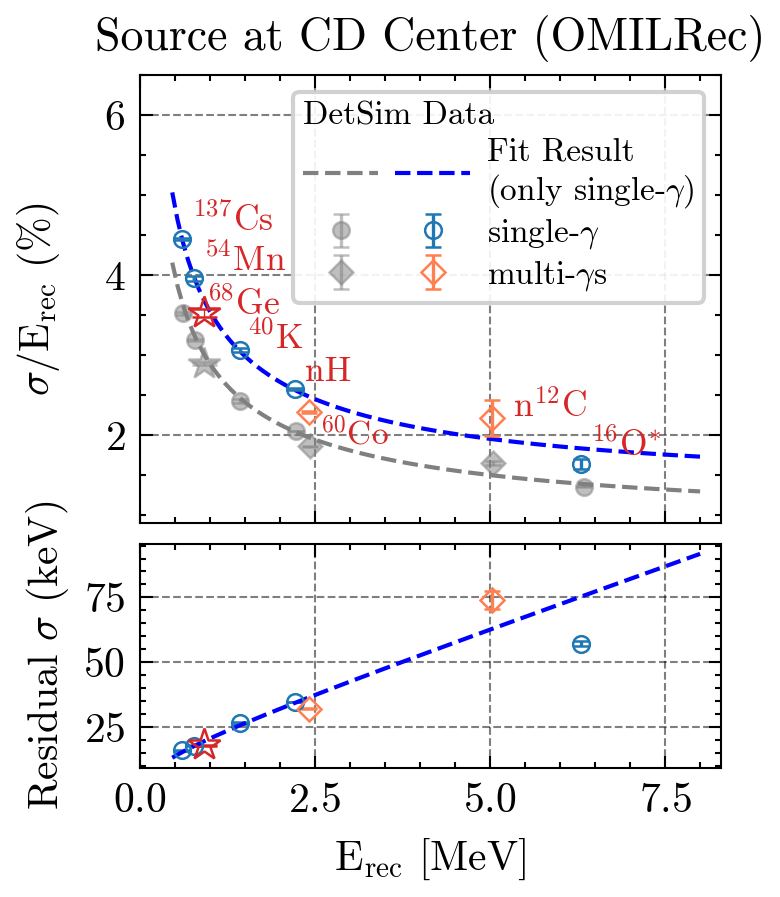
\includegraphics[width=0.85\textwidth]{4_efficiency/data_mc_resolution_center.png}
    \caption{Comparison of energy resolution between experimental data and detector simulation for sources at the detector center (OMILRec). \textbf{Top:} Relative energy resolution $\sigma/E_{\text{rec}}$ versus $E_{\text{rec}}$. Data points include single-$\gamma$ (blue circles) and multi-$\gamma$ sources (orange diamonds and red stars). The dashed line is a fit to the single-$\gamma$ simulation data. \textbf{Bottom:} Residual standard deviation $\sigma_{\text{res}} = \sqrt{\sigma_{\text{Data}}^2 - \sigma_{\text{MC}}^2}$ in keV. The residual is consistently above 15 keV and shows a positive trend with energy.}
    \label{fig:data_mc_comparison}
\end{figure}

\paragraph{Decomposition of the Residual Resolution}
To identify the physical origins of the excess resolution, a decomposition of $\sigma_{\text{res}}$ is performed. The methodology follows the framework established in previous CPC studies, where the total resolution is expressed as the quadrature sum of contributions from several independent effects. The decomposition formula is:
$$
\sigma_{\text{res}}^2 = \sigma_{\text{Vertex}}^2 + \sigma_{\text{Waveform}}^2 + \sigma_{\text{sPE Charge}}^2 + \sigma_{\text{Dark Noise}}^2 + \sigma_{\text{Other}}^2
$$
The contribution from Dark Noise ($\sigma_{\text{Dark Noise}}$) is not taken directly from simulation but is instead quantified using a toy MC method based on the high-statistics periodic trigger data as shown in Fig.~\ref{fig:periodic_trigger}, providing a more realistic estimate of its impact.

Fig.~\ref{fig:residual_decomposition} presents the result of this subtraction analysis. The black solid line represents the total $\sigma_{\text{res}}$. Starting from this total, the contributions from four key effects are sequentially subtracted in quadrature, following the order: Dark Noise, single Photoelectron (sPE) charge smear, waveform reconstruction inaccuracy, and vertex reconstruction uncertainty. The area between successive curves, filled with color, visually represents the magnitude of each contribution. The analysis indicates that the low-energy region ($E_{\text{rec}} < 1$ MeV) is dominated by the combined effects of Dark Noise and sPE charge smearing, which is well understood. However, the significant and increasing residual contribution in the high-energy region ($E_{\text{rec}} > 1$ MeV), which remains after accounting for these known effects, points to sources of systematic uncertainty that are currently not well modeled. This high-energy residual shows a clear proportionality to the incident energy.

\begin{figure}[h!]
    \centering
    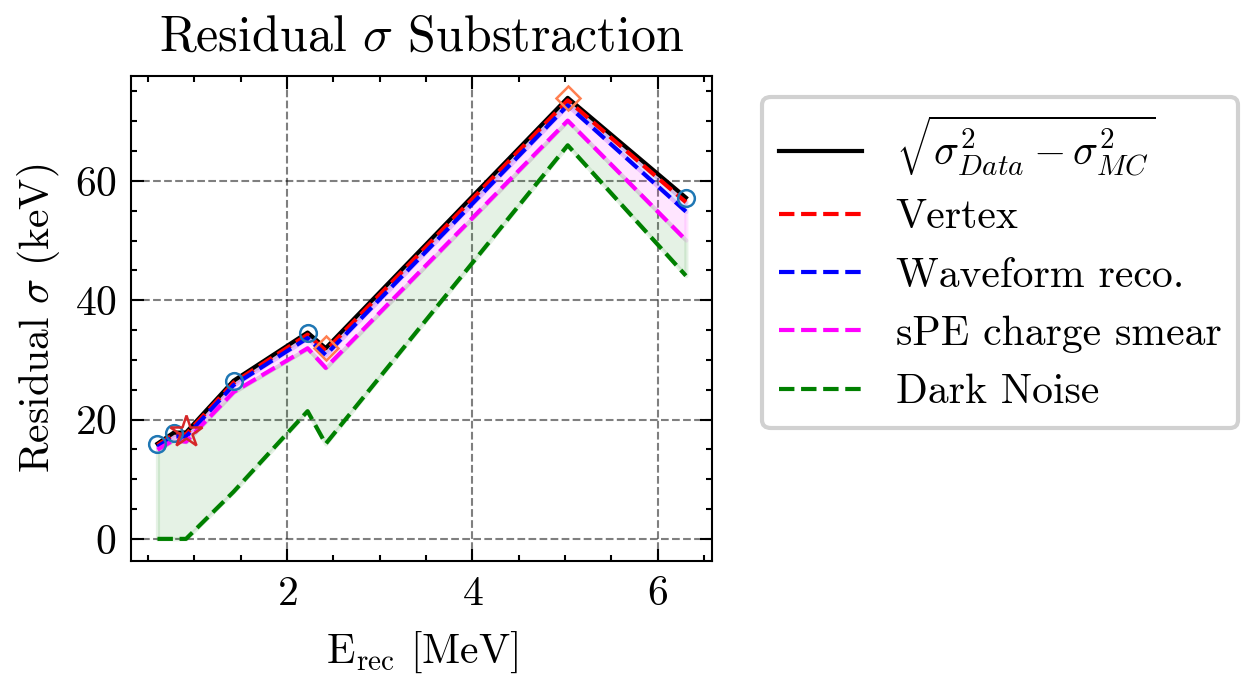
\includegraphics[width=0.7\textwidth]{4_efficiency/residual_sigma_subtraction.png}
    \caption{Decomposition of the residual energy resolution $\sigma_{\text{res}}$. The black solid line is the total $\sigma_{\text{res}} = \sqrt{\sigma_{\text{Data}}^2 - \sigma_{\text{MC}}^2}$. The colored dashed lines show the residual after sequentially subtracting, in quadrature, the contributions from: Dark Noise (estimated based on real data), sPE charge smearing (purple), waveform reconstruction (blue), and vertex reconstruction (red).}
    \label{fig:residual_decomposition}
\end{figure}

\paragraph{Future Work: Full-Chain Simulation and Quantification}
The origin of the energy-proportional residual contribution requires further investigation. We are currently developing a complete \textbf{full-chain simulation} workflow, encompassing the data-driven SPE model, to the application of the full reconstruction algorithms (including vertex and waveform reconstruction). This will help us quantify the intrinsic performance limits introduced by the SPE, waveform reconstruction, and energy-vertex reconstruction algorithms of OMILRec. 

\subsection{Reactor related uncertainty}
The accurate prediction of the reactor antineutrino flux and spectrum depends on several reactor-related parameters, each contributing to the total systematic uncertainty. These include the precise measurement of the reactor's thermal power, the understanding of the energy released per fission, the evolving fission fractions of the four primary isotopes throughout the fuel cycle, and corrections for effects like the non-equilibrium of long-lived fission fragments and the antineutrino emission from spent nuclear fuel. Comprehensive simulations of the reactor core, validated against operational data, are used to track the complex evolution of the fuel composition. The uncertainties from these reactor physics aspects are major contributors to the overall uncertainty in the predicted antineutrino signal at the JUNO experiment.

These uncertainties are kind of complicated and it is hard to define whether they are fully reactor-correlated or reactor-uncorrelated. 
Therefore, some tests are done by defining their reactor correlation and they are used to check which treatment is more conservative. 

\subsubsection{Reactor power}
Based on the experience from Daya Bay experiment, the thermal power of the reactor cores is mainly monitored by three systems. Accounting for correlations and calibration differences, the uncertainty of the KIT/KDO system, which provides hourly thermal power data to the experiment, is estimated to be 0.5\%. 
In this study, the reactor power uncertainties are handled core-by-core, assuming full correlation among cores within the same NPP and no correlation across different NPPs.

Some configurations are set and tests are done. 
\begin{itemize}
        \item Config. 1: Core-by-core uncorrelated 
        \[
        \chi^2_{\text{RUC}} = \sum_{r} \left( \frac{\alpha_r}{\sigma_r} \right)^2
        \]
        \item Config. 2: Core-by-core in same NPP correlated, but NPP-by-NPP uncorrelated 
        \[
        \chi^2_{\text{RUC}} = \sum_{p} \left( \frac{\alpha_p}{\sigma_p} \right)^2 
        \]
    \end{itemize}
    
    \vspace{0.5em}
    \begin{tabular}{|l|c|c|c|}
        \hline
        \textbf{50 days} & $\Delta m^2_{31}$ precision [\%] & $\sin^2\theta_{12}$ precision [\%] & $\Delta m^2_{21}$ precision [\%] \\
        \hline
        Config. 1 & 1.141 & 2.383 & 1.311 \\
        \hline
        Config. 2 & 1.141 & 2.386 & 1.311 \\
        \hline
    \end{tabular}
   
    It is found that the config. 2 produces a more conservative results. 


\subsubsection{Fission energy}
The energy released per fission for each isotope is defined as the energy converted to heat over a finite time, accounting for energy carried by neutrinos and captures on non-fissile materials. 
As studied by Daya Bay experiment, the fission energy is not a fixed fundamental constant but depends on the reactor environment.
In this study, the uncertainties of fission energy are handled assuming full correlation among cores.


\subsubsection{Fission fraction}
Electron antineutrinos are produced from the beta decays of fragments from four primary fission isotopes: $^{235}\rm U$, $^{238}\rm U$, $^{239}\rm{Pu}$, $^{241}\rm{Pu}$. Their relative contributions, or fission fractions change dynamically with fuel burn-up. 
The Daya Bay nuclear power plant provides detailed simulations of this evolution using the validated SCIENCE/APOLLO2 software package. Comparisons between APOLLO2 calculations and direct measurements of spent fuel isotopic content show deviations of less than 5\%. 
Therefore, the uncertainty for each fission fraction is conservatively estimated to be 5\%. These fractions are strongly correlated, as the consumption of uraiunm and production of plutonium isotopes are linked. A correlation matrix is used for proper uncertainty propagation.
JUNO alaysis follows the similar strategy as the Daya Bay analysis. 
In this study, the uncertainties of fission fractions are handled assuming full correlation among cores.


\subsubsection{Spent fuel}
Long-lived fission isotopes within the spent nuclear fuel(SNF) continue to beta-decay, producing an additional source of antineutrinos. The contribution from SNF is calculated by identifying isotopes with half-lives longer than 10 hours and whose decays exceed the inverse beta decay threshold. Using the refueling history and SNF inventory provided by the plant, the cumulative yield and spectrum of these isotopes are computed. 
In this study, the rate uncertainties of SNF spectrum are handled core-by-core, assuming full correlation among cores within the same NPP and no correlation across different NPPs. The shape uncertainties are neglected.


\subsubsection{Non-equilibrium}
The long-lived fission fragments need some time to reach equilibrium between their production and decay rates. 
In an operating reactor core, these fragments accumulate, and their decays contribute extra antineutrinos, known as the non-equilibrium (NonEq) contribution.
In this study, the rate uncertainties of NonEq spectrum are handled core-by-core, assuming full correlation among cores within the same NPP and no correlation across different NPPs. The shape uncertainties are neglected.

\subsubsection{Reference spectrum}
Systematic uncertainties in the IBD yield is dominated by the reference spectrum used in this analysis, which is measured with an uncertainty of 1.2\% from the DayaBay paper~\cite{DYB:Flux2025}.
The IBD yield,  $5.84 \pm 0.07 \times 10^{-43}$~cm$^2$/fission, includes the uncertainties from the IBD cross section, the thermal power, fission fractions and fission energy from Daya Bay and Lingao reactor power plant.
The uncertainty of the IBD cross section is fully correlation between Daya Bay and JUNO, and thus shall not consider the cross section uncertainty in JUNO.
Weighted by the thermal power and baseline of each reactor core or nuclear power plant, the average fission fractions in the JUNO data were 0.564, 0.076, 0.303, and 0.058 for $^{235}$U, $^{238}$U, $^{239}$Pu, and $^{241}$Pu, respectively. In comparison, the corresponding values in the Daya Bay data were 0.564, 0.076, 0.304 and 0.056~\cite{DYB:Flux2025}.
Consequently, they shared a $>$\,99\% common reactor antineutrino spectrum, which we denote as the model-independent component shared by both the JUNO and Daya Bay datasets.
The differences in the fission fractions between JUNO and Daya Bay resulted in a $<$0.1\% uncertainty in the flux, assuming a 10\% uncertainty in the isotopic reference spectra.


\subsubsection{Summary}

\begin{table}[!htbp]
    \caption{Summary of the systematic uncertainties of the predicted integrated reactor antineutrino flux associated with a single reactor core.}
    \label{tab:reactorErr}
    \centering
    \footnotesize% fontsize
    \setlength{\tabcolsep}{4pt}% column separation
    \renewcommand{\arraystretch}{1.2}%row space 
    \begin{tabular}{lc}
        \hline
        Parameter & Uncertainty \\ 
        \hline
        power & 0.5\% \\
        energy/fission & 0.2\% \\
        reference spectrum & 1.2\% \\
        different fission fraction & 0.1\% \\
        fission fraction & 0.6\% \\
        spent nuclear fuel & 0.3\% \\
        non-equilibrium & 0.2\% \\
        \hline 
    \end{tabular}
\end{table}

